%% LyX 2.2.4 created this file.  For more info, see http://www.lyx.org/.
%% Do not edit unless you really know what you are doing.
\documentclass[oneside,brazil]{extbook}
\renewcommand{\familydefault}{\sfdefault}
\usepackage[T1]{fontenc}
\usepackage[utf8]{inputenc}
\setcounter{secnumdepth}{3}
\setcounter{tocdepth}{3}
\usepackage{color}
\usepackage{babel}
\usepackage{float}
\usepackage{textcomp}
\usepackage{graphicx}
\usepackage[unicode=true,
 bookmarks=true,bookmarksnumbered=true,bookmarksopen=true,bookmarksopenlevel=2,
 breaklinks=false,pdfborder={0 0 0},pdfborderstyle={},backref=false,colorlinks=true]
 {hyperref}
\hypersetup{
 pdfauthor={Ricardo JL Rufino},
 linkcolor=blue, urlcolor=magenta, citecolor=blue}
\usepackage{breakurl}

\makeatletter

%%%%%%%%%%%%%%%%%%%%%%%%%%%%%% LyX specific LaTeX commands.
\newcommand{\noun}[1]{\textsc{#1}}
%% Because html converters don't know tabularnewline
\providecommand{\tabularnewline}{\\}
\floatstyle{ruled}
\newfloat{algorithm}{tbp}{loa}[chapter]
\providecommand{\algorithmname}{Algoritmo}
\floatname{algorithm}{\protect\algorithmname}

%%%%%%%%%%%%%%%%%%%%%%%%%%%%%% User specified LaTeX commands.
\usepackage{acronym}
\usepackage{listings}
\usepackage{color}

\definecolor{dkgreen}{rgb}{0,0.6,0}
\definecolor{gray}{rgb}{0.5,0.5,0.5}
\definecolor{mauve}{rgb}{0.58,0,0.82}

\lstset{
  %frame=tb,
  language=Java,
  aboveskip=3mm,
  belowskip=3mm,
  showstringspaces=false,
  columns=flexible,
  basicstyle={\small\ttfamily},
  numbers=none,
  numberstyle=\tiny\color{mauve},
  keywordstyle=\color{blue},
  commentstyle=\color{gray},
  stringstyle=\color{dkgreen},
  breaklines=true,
  breakatwhitespace=true,
  tabsize=3
}


% foi desabilitada a fonte padrão no Lyx : http://tex.stackexchange.com/a/88295
% e foi configurado Unicode UTF-8

%% fazer o template book reconhecer os keywords do resumo.
\def\keywords{\vspace{.5em}
{\textit{Keywords}:\,\relax%
}}
\def\endkeywords{\par}

\makeatother

\usepackage{listings}
\renewcommand{\lstlistingname}{\inputencoding{latin9}Listagem}

\begin{document}

\title{OpenDevice: Uma Plataforma Aberta e Framework para Internet das Coisas
(IoT)}

\maketitle
\tableofcontents{}

\listoffigures


\section*{Acrônimos}

\begin{acronym}[ACRONYM] 
  
\acro{IoT}{Internet Of Things}
\acro{JVM}{Java Virtual Machine}
\acro{MQTT}{MQ Telemetry Transport}
\acro{REST}{Representational State Transfer}
\acro{HTTP}{Hypertext Transfer Protocol}
\acro{RAM}{Random Access Memory}
\acro{JNI}{Java Native Interface}
\acro{API}{Application Programming Interface}
\acro{UDP}{User Datagram Protocol}
\acro{UART}{Universal Asynchronous Receiver/Transmitter}
\acro{USB}{Universal Serial Bus}
\acro{EPROM}{Erasable Programmable Read-Only Memory}
\acro{RFID}{Radio Frequency Identification}
\acro{ISR}{Interrupt Service Routine}
\acro{IDE}{Integrated Development Environment}
\acro{GPIO}{General Purpose Input/Output}
\acro{PCB}{Printed Circuit Board}
\acro{LED}{Light Emitting Diode}


\end{acronym}



\section*{Resumo}

A Internet das Coisas (IoT) é uma área que vem atraindo a atenção
tanto do meio acadêmico quanto da indústria e demanda uma complexa
arquitetura com diversos componentes, que integram hardwares, sensores
e atuadores dos mais variados protocolos e interfaces. A Internet
das Coisas irá mudar a forma como nos comportamos e interagimos com
o ambiente, gerando novos serviços nas áreas da saúde, educação, lazer,
esportes, automação, etc. 

Por ser uma área relativamente nova, vem sofrendo também com os problemas
devido à falta de padronização. Dessa forma, a criação de projetos
de IoT se tornam desafiadores, com custo e tempo elevados ou acabam
tendo uma baixa qualidade, pois os desenvolvedores têm que resolver
problemas comuns, porém complexos, como definição de protocolos e
gerenciamento de dispositivos, o que atrasa o desenvolvimento e a
geração de soluções inovadoras.

Nesta dissertação propõe-se um framework completo e flexível que auxilia
no desenvolvimento de soluções de Internet das Coisas, como: automação
residencial, monitoramento de sensores, controle de robôs, monitoramento
de energia e cidades inteligentes, abordando todas as plataformas
envolvidas: Desktop, Web, Mobile, Hardware e oferecendo serviços para
gerenciamento de dispositivos, conexões, armazenamento de dados e
visualização, bem como a proposta de um protocolo para a comunicação
com hardwares de baixo custo, baseados na plataforma Arduino, ESP8266,
Raspberry Pi e similares, podendo operar usando as tecnologias USB,
Bluetooth, Ethernet, WiFi e com protocolos abertos, como MQTT e WebSocket.

Foram implementados cenários no contexto de automação residencial/predial
e integração com plataformas 3D, para avaliar a proposta da arquitetura
e componentes, partindo de uma aplicação mais simples para uma aplicação
mais complexa. Os experimentos permitiram concluir que os componentes
da arquitetura fornecem a abstração e a extensibilidade necessária
para implementar projetos de IoT no contexto de automação, e que os
componentes da arquitetura impactam minimamente na performance do
projeto.

\begin{keywords}
Internet das Coisas, IoT, Framework, Middleware, Arduino, MQTT, Sistemas Embarcados, Automação Residencial.
\end{keywords}



\chapter{Introdução}

A Internet das Coisas ou Internet of Things (IoT)\cite{Ashton2009},
em inglês, é um termo utilizado para descrever um paradigma tecnológico
no qual os objetos físicos estão conectados em rede e se comunicam
através da Internet, gerando informações, atuando de forma inteligente
a eventos, integrando aplicações e serviços.

A IoT é umas das principais tecnologias emergentes, é considerada
a terceira onda de desenvolvimento da Internet\cite{GoldmanSachs2014},
e assim como as duas primeiras ondas, promete trazer profundas mudanças
na economia. Essa ``revolução'' vem impulsionando mudanças nos padrões
da própria Internet, a fim de atender uma escala nunca antes vista
de ``coisas'' conectadas, e inevitavelmente, promovendo para vida
cotidiana, trabalho, saúde e negócios.

Recentes avanços tecnológicos tem impulsionado o desenvolvimento da
Internet das Coisas, a citar: (1) redução dos custos de sensores e
microprocessadores, permitindo a criação de dispositivos ``mais inteligentes'',
(2) redução no custo de banda da internet, algo estimado em 40x nos
últimos 10 anos, (3) a presença massiva de smartphones, tornando-se
uma ferramenta para geração de dados, visualização e controle, (4)
BigData, com a capacidade de processar enorme quantidades de dados
e gerar informações estratégicas para os negócios e (5) a alta disponibilidade
de acesso a rede internet de maneira quase ubíqua\cite{GoldmanSachs2014}.

O potencial estimado da Internet das Coisas tem despertado o interesse
e investimento de grandes empresas como Google, Microsoft, Intel,
Oracle, IBM, Cisco, Sansung. Não somente empresa, mas projetos e
fundações ligadas ao ``ecossistema'' open source, como Eclipse,
Arduino, Ubuntu/Linux, vem apostando na Internet das Coisas. 

Apesar dos benefícios e oportunidades, ainda existem uma série de
desafios que precisam ser superados para uma transição completa para
a Internet das Coisas\cite{mattern2010,teixeira2011}. Os desafios
estão relacionados à heterogeneidade, escalabilidade, interoperabilidade
, segurança, privacidade, grande volumes de dados, complexidade do
software e do hardware, que estão inseridos com graus de relevâncias
diferenciados nas áreas da saúde, transportes, telecomunicações, automação,
etc.

Um enorme esforço de investigação é necessário para fazer a IoT viável,
uma vez que muitas questões em aberto ainda persistem nesta área.
A comunidade científica está oferecendo várias tentativas para padronizar
totalmente o paradigma IoT. Além disso, o grande número de dispositivos
que são esperados integrar o ambiente de IoT, obriga um esquema de
endereçamento eficaz. Tais questões são geralmente discutidos na literatura\cite{yang2010,Katasonov2008}. 

\section{Motivação}

A Internet das Coisas é uma grande oportunidade para empresas e desenvolvedores
criarem novas soluções que conectem dispositivos à Internet. Novos
dispositivos, sensores, microcontroladores e plataformas de desenvolvimento
vêm surgindo, impulsionados por essas oportunidades e pelo desenvolvimento
da Internet das Coisas. Porém, essa grande quantidade de dispositivos
heterogêneos, decorrente da inerente diversidade de tecnologias de
hardware e software, se tornam um dos principais desafios para o desenvolvimento
de aplicações.

Devido à falta do estabelecimento de padrões das plataformas de hardware
e software, os desenvolvedores acabam criando suas próprias soluções,
o que contribui para o problema da interoperabilidade. Muitas das
soluções elaboradas, acabam tendo uma baixa qualidade, são fechadas
(proprietárias) ou devido a sua complexidade acabam atrasando ou mesmo
inviabilizando o atendimento dos principais requisitos, que é gerar
valor de mercado e promover a inovação.

Nesse contexto, plataformas de middleware são avaliadas como soluções
promissoras para prover tal interoperabilidade, realizar o gerenciamento
da crescente quantidade de dispositivos e integrar aplicações\cite{teixeira2011}.
Tais plataformas oferecem um meio padronizado para o acesso aos dados
e serviços através de uma interface de alto nível\cite{Bandyopadhyay2011},
com isso as aplicações não precisam lhe dar com os detalhes de baixo
nível relacionados às especificidades de cada dispositivo e padrões
de comunicação. A adoção de uma plataforma de middleware, pode contribuir
para facilitar o desenvolvimento de projetos de IoT.

Existem cerca de 9 milhões de desenvolvedores Java, o fornecimento
de frameworks e serviços \emph{open source} em plataforma Java irá
tornar mais fácil a adoção da linguagem para projetos de Internet
das Coisas e favorecer possíveis contribuições para o desenvolvimento
e aprimoramento da solução proposta nesse trabalho.

\subsection{Desafios}

Sistemas baseados em Internet das Coisas podem ser usado para diferentes
fins e áreas, de modo que, temos de enfrentar diferentes desafios.
Nesta seção, vamos explicar alguns dos desafios que precisam ser considerados
nas atividades de investigação:
\begin{itemize}
\item \textbf{Tecnologias de Borda:} Ao nível do hardware, são necessários
mais esforços de investigação para desenvolver a tecnologia de dispositivos
embarcados, sensores, atuadores e identificação (passiva e ativa),
uma vez que um sistema baseado na Internet das Coisas deve ser capaz
de reunir informações suficientes sobre o mundo real, empregando uma
grande variedade de dispositivos e ambientes. Assim, exige-se mais
esforços para conectar dispositivos heterogêneos e implantá-los em
aplicações da Internet das Coisas, e para fornecer suporte para novos
dispositivos.
\item \textbf{Tecnologias de Rede}: Em IoT, as coisas estão ligadas através
de diferentes tipos de redes, ou seja, rede móvel, com e sem fio.
Estas redes fornecem comunicação bidirecional em diferentes níveis
entre os objetos do mundo real, aplicações e serviços que são utilizados
pelas aplicações da Internet das Coisas. Esta estrutura altamente
distribuída deve fornecer interconexão com baixo consumo de energia,
enquanto os dados distribuídas podem causar problemas de privacidade.
\item \textbf{Middleware:} Em IoT, temos redes e dispositivos heterogêneos.
Sua heterogeneidade pode potencialmente aumentar com as novas tecnologias.
Para facilitar a utilização destes dispositivos por aplicações da
Internet das Coisas, devemos proteger a sua heterogeneidade. Portanto,
precisamos desenvolver um middleware seguro, escalável e semanticamente
enriquecido para lidar com a heterogeneidade dos dispositivos.
\item \textbf{Plataformas de Serviços:} Eles suportam uma gestão de alto
nível de todos os dispositivos envolvidos, de forma integrada, garantindo
a escalabilidade, alta disponibilidade, e a execução segura das funcionalidades
solicitadas a partir de dispositivos.
\end{itemize}

\section{Objetivo Geral\label{sec:Objetivos}}

Criação de um framework para facilitar o desenvolvimento de aplicações
para Internet das Coisa, com menor custo e tempo possível, abstraindo
dispositivos, protocolos e tecnologias de comunicação de comunicação,
bem como oferecer um conjunto de APIs para integração com outras aplicações.

\section{Objetivos Específicos}

Os objetivos específicos que este trabalho pretende alcançar, são
listador a seguir:
\begin{itemize}
\item \textbf{Solução completa para integração entre plataformas}: oferecendo
soluções para o desenvolvimento e integração de projetos nas plataformas
de Hardware, Desktop, Web e Mobile.
\item \textbf{Integração entre diferentes dispositivos e protocolos}: permitindo
integrar diferentes dispositivos e protocolos em um mesmo ambiente
de maneira transparente e consistente, focando em padrões abertos
e baseado em plataformas open source (hardware e software). 
\item \textbf{Utilização em dispositivos com limitações de processamento
e memória}: oferecer soluções para o desenvolvimento de dispositivos
embarcados com limitações de processamento e memória, como microcontroladores
(AVR 8-bits), mini PCs e dispositivos móveis.
\item \textbf{Oferecer um protocolo aberto e extensível}: Trata-se da elaboração
de um protocolo (baseado em comandos), para integrar aplicações e
dispositivos com limitações de memória e processamento, permitindo
uma comunicação bidirecional, em tempo-real e apoiada sobre padrões
abertos como MQTT, WebSocket, TCP, etc. Um dos principais objetivos
é que este protocolo seja de fácil implementação e extensível.
\item \textbf{Simplificação na criação de dispositivos inteligentes}: permitindo
que as empresas e indivíduos possam focar em questões de projeto,
design, marketing e comercialização dos novos dispositivos inteligente
que irão compor a Internet das Coisas.
\item \textbf{Oferecer uma plataforma base para criação de projetos especializados}:
através de uma arquitetura flexível, oferecer uma fundação para que
empresas e desenvolvedores possam estender a adaptá-la a regras de
casos de uso específicos das áreas de automação, transporte, cidades
inteligentes, etc.
\end{itemize}
Neste contexto é apresentado o OpenDevice, um framework que facilita
a criação de projetos de Internet das Coisas usando tecnologias de
baixo custo, como: Arduino\cite{url:arduino:intro}, Rasberry Pi\cite{url:raspberry},
ESP8266\cite{url:esp8266:espressif} e outros\cite{arduino-comp1,arduino-comp2,arduino-comp3}.

\section{Organização da Dissertação}

Este trabalho está organizado da seguinte forma. O capítulo 2 apresenta
os fundamentos para o desenvolvimento desta dissertação. O capítulo
3 apresenta e discute propostas e trabalhos relacionados com o desenvolvimento
de middlewares ou projetos correlacionados. O capítulo 4 apresenta
a arquitetura proposta e os seus componentes, assim como a implementação
dessa arquitetura. O capítulo 5 apresenta a avaliação e os testes
da implementação da proposta. Finalmente, o capítulo 6 apresenta as
conclusões da dissertação, assim como os trabalhos futuros. 



\chapter{Fundamentação Teórica}

\section{Internet das Coisas}

O termo Internet das Coisas (em inglês, Internet of Things - IoT),
foi usado pela primeira vez em 1999 pelo pesquisador britânico Kevin
Ashton\cite{Ashton2009}. O autor descreve a Internet das Coisas como
um sistema através do qual os objetos do nosso cotidiano possam se
conectar à internet usando sensores. Ashton aplicou esse termo para
explicar o poder da conectividade das tags de rádio frequência identificada
(RFID), usadas pelas grandes empresas para contagem de estoques sem
a necessidade da interferência humana.

Em \cite{santos2014}, os pesquisadores definem IoT como “uma rede
de objetos interconectados, os quais poderiam possuir seus próprio
endereço de IP, estar incorporados a sistemas complexos e usar sensores
para monitorar o ambiente, respondendo a mudanças de contexto”. Tais
pesquisadores ainda avaliam a Internet das Coisas em quatro aspectos.
O primeiro é a possibilidade de seus sistemas conduzirem seus processos
de forma independente da Internet atual. O segundo é que a IoT é construída
em conjunto com novos serviços. O terceiro é que ela serve como ponte
de comunicação não somente entre pessoas e objetos, mas também entre
objetos e objetos (M2M ou Machine-to-Machine), e por último é que
as redes podem ser abertas (públicas) ou fechadas (privadas ou restritas
somente para alguns dispositivos).

A internet revolucionou a forma como as pessoas se comunicam em escala
global, o próximo passo é intercomunicar as ``coisas''. Os recentes
avanços na tecnologia de sistemas micro-eletro-mecânicos nas comunicações
sem fio e na eletrônica digital, possibilitaram a construção de microcontroladores
e sensores de tamanho e custo reduzidos. A proliferação destes dispositivos
em uma rede de comunicação cria a chamada Internet das Coisas (IoT).

Na última edição do IoT World Forum, realizada de entre 6 e 8 de dezembro
de 2015 em Dubai\cite{url:computerworld:2015,url:webintel:2015,url:cisco:iot:2015},
foram divulgados alguns dados que demostram o tamanho do crescimento
da IoT. Entre eles:
\begin{itemize}
\item 58\% das empresas do mercado dizem que IoT é estratégico para seu
futuro (se tiver, uma referência mais específica); 
\item Atualmente o crescimento de sistemas de IoT tem dobrado ano a ano; 
\end{itemize}
Crescimento da IoT entre 2013 e 2015:
\begin{itemize}
\item Sensores colocados no mercado: 10 bilhões em 2013 e 55 bilhões em
2015; 
\item Conexões de IoT: 11 bilhões em 2013 e 18 bilhões em 2015; 
\item Conexões M2M: 43 bilhões em 2013 e 73 bilhões em 2015; 
\item Empresas participantes em consórcios e associações da IoT: 44 em 2013
e 354 em 2015;
\end{itemize}
Investimentos:
\begin{itemize}
\item Desenvolvedores focados em IoT: 291 mil em 2013 e 813 mil em 2015; 
\item Startups em IoT: 127 em 2013 e 1.502 em 2015;
\item Investimentos de Capital de Risco: US\$1,1 bilhão em 2013 e US\$ 2
bilhões em 2015;
\end{itemize}
Oportunidades:
\begin{itemize}
\item Receita gerada por IoT: US\$ 548 bilhões em 2013 e US\$ 780 bilhões
em 2015; 
\item Receita de serviços de M2M: US\$ 79 bilhões em 2013 e US\$ 122 bilhões
em 2015;
\item “Coisas” não conectadas em 2013: 99,25\% e em 2015 98,85\%.
\end{itemize}
Previsão para o ano 2020:
\begin{itemize}
\item 50 bilhões de “coisas” conectadas; 
\item 6 dispositivos por pessoa;
\item US\$ 11 trilhões de dólares em novos negócios. 
\end{itemize}
Vários protocolos de aplicação divergentes têm sido propostos para
Internet das Coisas, incluindo CoAP, REST, XMPP, AMQP, MQTT, DDS e
outros. Cada protocolo incide sobre um aspecto específico das comunicações
da Internet das Coisas. A falta de um protocolo que possa lidar com
as exigências verticais de mercado de aplicações da Internet das Coisas,
incluindo máquina-a-máquina, máquina-servidor, e comunicações de servidor
para servidor resultou em uma fragmentação do mercado entre muitos
protocolos. Por sua vez, esta fragmentação é um obstáculo principal
no desenvolvimento de novos serviços que exigem a integração de múltiplos
serviços da Internet das Coisas para desbloquear novas capacidades
e proporcionar uma integração horizontal entre os serviços.

Diferentes organismos de normalização e grupos estão ativos na criação
de pilhas de protocolo mais interoperáveis e de normas abertas para
a Internet das Coisas. À medida que avançamos a partir do HTTP, TCP
e IP para uma pilha de protocolos específicos para Internet das Coisas,
eventualmente, nos deparamos com uma sopa de acrônimos de protocolos
sem fio, como ZigBee, RFID, Bluetooth, e BACnet às normas de protocolo
de última geração, tais como 802.15.4e, 6LoWPAN, RPL, e CoAP, que
tentam unificar as redes de sensores sem fio e a Internet\cite{electronicdesign:2016}. 

Por definição, a Internet das Coisas tem um enorme abrangência, que
pode ser difícil de atender através de um única solução. A IoT pode
ser dividida em cinco principais setores (Figura \ref{fig:iot-report}),
que seriam as principais verticais de adoção da IoT\cite{Goldman2014}:
dispositivos vestíveis (\emph{Wearables}), carros conectados, casas
conectadas, cidades conectadas e Industriais.

\begin{figure}
\begin{centering}
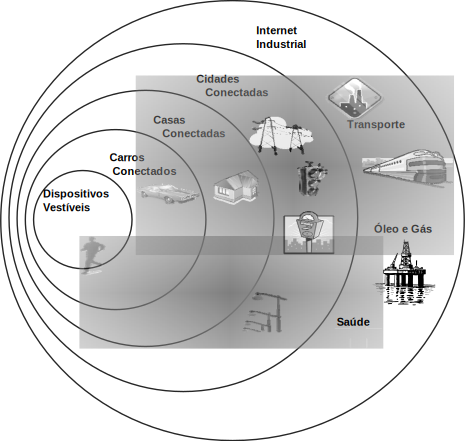
\includegraphics[width=0.7\linewidth]{Imagens/Cap_2/iot-report}
\par\end{centering}
\caption[Principais áreas de adoção]{ Principais áreas de adoção (traduzido e adaptado de \cite{Goldman2014})\label{fig:iot-report}}
\end{figure}

Na abertura do evento IoT Week 2013, Ashton afirmou que \textquotedbl{}A
IoT é aqui e agora; não é o futuro, mas o presente\textquotedbl{}\footnote{http://kevinjashton.com/2013/06/17/pre-recorded-opening-talk-for-internet-of-things-week-helsinki-
june-17-2013/}.


\section{Sistemas Embarcados}

Um sistema embarcado é uma combinação de hardware e software, projetados
para executar uma função específica \cite{Noergaar2005}. Como acontece
com qualquer sistema eletrônico, este sistema requer uma plataforma
de hardware construída com um microprocessador ou microcontrolador.
O hardware do sistema embarcado inclui elementos como interface do
usuário, interfaces de entrada/saída (I/O), display, memória, etc.
Geralmente, um sistema embarcado é composto por uma fonte de alimentação,
processador, memória, temporizadores, portas de comunicação serial
e circuitos específicos da aplicação do sistema.

Sistemas embarcados são mais limitados em hardware e software do que
um computador pessoal (PC). Em termos de limitações de hardware, isto
pode significar limitações no desempenho de processamento, o consumo
de energia, memória, e assim por diante\cite{Noergaar2005}.

\subsection{Tipos de Sistemas Embarcados}

Sistemas embarcados podem ser classificados em diferentes tipos: com
base no desempenho, requisitos funcionais e de desempenho do microcontrolador.

\begin{figure}[h]
\begin{centering}
\includegraphics[width=1\linewidth]{Imagens/Cap_2/embedded-systems-types}
\par\end{centering}
\caption{Tipos de Sistemas Embarcados \cite{url-efxkits} \label{fig:embedded-systems-types}}
\end{figure}

Sistemas embarcados são classificados em quatro categorias com base
em seu desempenho e requisitos funcionais:
\begin{itemize}
\item Sistemas embarcados autônomos;
\item Sistemas embarcados em tempo real; 
\item Sistemas embarcados em rede; 
\item Sistemas embarcados móveis.
\end{itemize}
Sistemas embarcados são classificados em três tipos, com base no desempenho
do microcontrolador, tal como:
\begin{itemize}
\item Sistemas embarcados de pequena escala; 
\item Sistemas embarcados de média escala; 
\item Sistemas embarcados sofisticados.
\end{itemize}
Neste trabalho, abordaremos com mais ênfase os sistemas embarcados
de pequena escala, compreendendo os microcontroladores, e os de média
escala, compreendendo os mini PCs.

\subsection{Microcontroladores}

Um microcontrolador é um sistema computacional completo, no qual estão
incluídos uma CPU (Central Processor Unit), memória de dados e programa,
um sistema de clock, portas de entrada/saída (I/O), além de outros
possíveis periféricos, tais como, módulos de temporização e conversores
A/D entre outros, integrados em um mesmo componente\cite{Chou1992}.

Os sistemas micro-controlados estão presentes nas mais diversas áreas,
dentre as quais estão a automação industrial, automação comercial,
automação predial, área automobilística, agrícola, produtos manufaturados,
eletrodomésticos, telecomunicações, etc. A Texas Instruments é creditada
com a criação do primeiro microcontrolador, a série TMS1000. Os microcontroladores
série TMS1000 tiveram bastante RAM, ROM e I/O e foram usados como
controladores de forno de micro-ondas, em temporizadores industriais,
e em calculadoras\cite{Gadre2000}.

Em geral, os microcontroladores são projetados para serem fáceis de
utilizar, do ponto de vista do projetista de circuitos. A Figura \ref{fig:microcontroller}
representa o diagrama de blocos do que um microcontrolador típico,
especialmente, os da série PIC. Um microcontrolador pode fazer interface
com motores, displays, leitura de sensores externos, realizar a comunicação
com um PC e mesmo se conectar a uma rede de controladores semelhantes,
e pode fazer tudo isso sem uma quantidade excessiva de componentes.
Isto leva a um pequeno e compacto sistema que é mais confiável e de
baixo custo.

\begin{figure}[h]
\begin{centering}
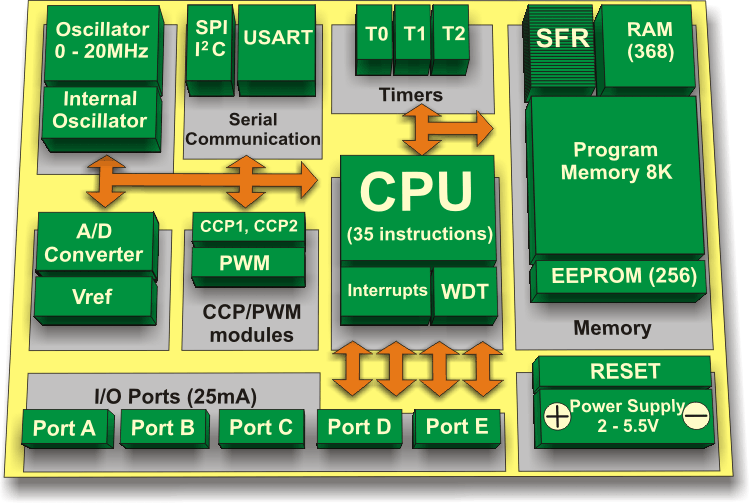
\includegraphics[width=0.8\linewidth]{Imagens/Cap_2/microcontrroler_pic}
\par\end{centering}
\caption{Diagrama de Blocos - PIC16F887 \cite{MilanVerle2008} \label{fig:microcontroller}}
\end{figure}

Em seguida, apresentamos os componentes do microcontrolador.
\begin{itemize}
\item \textbf{CPU:} A unidade central de processamento (CPU) é o coração
do controlador. Ela obtém as instruções armazenadas na memória de
programa, decodifica essas instruções, e executa. A CPU em si é composto
de registradores, a unidade lógica aritmética (ALU), decodificador
de instrução, e circuitos de controle.
\item \textbf{Memória de Programa}: A memória de programa armazena as instruções
que formam o programa. Para acomodar programas maiores, a memória
de programa pode ser particionada como memória de programa interno
e externo em alguns controladores. A memória de programa é geralmente
não volátil e pode ser EPROM, EEPROM, Flash, Mask ROM ou OTP (one-time
programmable).
\item \textbf{RAM}: A memória RAM é a memória de dados do controlador, ou
seja, ela é usada pelo controlador para armazenar dados. A CPU usa
memória RAM para armazenar variáveis, bem como a pilha. A pilha é
usada pelo processador para armazenar endereços de retorno a partir
de onde pode retomar a execução depois de ter completado uma sub-rotina
ou uma chamada de interrupção.
\item \textbf{Oscilador e Clock}: O controlador executa o programa a uma
determinada taxa. Esta velocidade é determinada pela frequência do
oscilador. O oscilador pode ser um oscilador RC-interno ou um oscilador
com um elemento de sincronismo externo, tal como um cristal de quartzo.
Assim que a energia é aplicada ao controlador, o oscilador começa
a funcionar.
\item \textbf{Porta Serial}: Ela é usada para se comunicar com dispositivos
externos através de uma comunicação serial, onde os dados são enviados
ou recebidos em 1 bit de cada vez. A porta serial pode operar em qualquer
velocidade de transferência, porém as mais usadas são 9800bps e 115200bps.
As portas seriais são de dois tipos: síncronas e assíncronas. A transferência
de dados síncrona precisa de um sinal de relógio (clock), para realizar
a ``sincronização'' do envio dos bits de dados, enquanto a transferência
de dados assíncrona não precisa do sinal do relógio, e a informação
de sincronização está incorporado nos dados, utilizando bits de controle
no início (START bit) e fim (STOP bit) do bloco de dados, que geralmente
é de 8-bits. O bit START é sempre baixo (0), enquanto o bit STOP é
sempre elevado (1).
\item \textbf{Porta I/O Digital}: O microcontrolador usa os componentes
de I/O (Entrada/Saída) digitais para a troca de dados digitais com
o mundo exterior. 
\item \textbf{Porta I/O Analógica}: A entrada analógica é realizada utilizando
um conversor analógico-digital (ADC). ADCs são usados para adquirir
dados analógicos de dispositivos, como sensores de temperatura e sensores
de pressão. A saída analógica é realizada utilizando um conversor
digital-para-analógico (DAC). A maioria dos controladores estão equipados
com moduladores de largura de pulso (PWM) que pode ser usado para
obter uma tensão analógica.
\item \textbf{Timer}: O \emph{timer} é usado pelo controlador para execução
de eventos baseados no tempo; por exemplo, realizar o controle de
velocidade de um motor, o brilho de um LED ou gerar um pulso PWM.
O \emph{timer} também pode ser usado para contar os eventos externos,
bem como internos, nesse caso, o temporizador é chamado um contador.
A quantidade de \emph{timers} disponíveis depende do microcontrolador
usado.
\item \textbf{Watchdog Timer}: O \emph{watchdog timer} (WDT) é um temporizador
especial, e geralmente é usado para prevenir falhas de software. Ele
funciona da seguinte forma: Uma vez armado, se o programa de usuário
não reiniciar o contador, notificando que tudo está certo, em um tempo
máximo predefinido, o contador estoura, ocorrendo o reset do microcontrolador.
A suposição é que, se o programa do usuário não repõe o WDT, ele falhou
de alguma maneira e, portanto, em vez de uma falha no sistema ou manter
um desempenho indesejado, é melhor reiniciar o sistema.
\end{itemize}

\subsection{Mini PCs}

Primeiramente, precisamos esclarecer que mini PCs não são os desktops
comuns, que já estão no mercado há alguns anos com placas-mãe pequenas
como micro ATX e flexATX. Estes, muito comuns em caixas de supermercado,
por exemplo, são apenas versões um pouco reduzidas dos computadores
comuns.

O tipo de máquina que estamos nos referindo são os credit-card sized
SBCs (single-board computers ou computadores de placa única do tamanho
de cartões de crédito). Além de serem super compactos, estes mini-pcs
foram desenhados especificamente para serem flexíveis e fáceis de
utilizar em projetos diversos por desenvolvedores, educadores e hobistas.
Suas dimensões não ultrapassam os 8 ou 9 centímetros de lado e, como
o nome já bem diz, possuem todos os seus componentes integrados em
uma única placa de circuito. São também muito eficientes no consumo
de energia, dispensando as complicadas e volumosas fontes dos PCs
comuns e utilizando portas USB ou carregadores padrão para sua alimentação.
Ainda assim, possuem opções de expansão e conectividade bem completas,
como entrada e saída de áudio, cartão SD, portas USB, saída HDMI e
rede ethernet.

Uma categoria especifica de mini PCs, voltada para desenvolvimento
de projetos embarcados, vem surgindo com o advento da Internet das
Coisas. Os avanços na tecnologia não permitiram apenas a miniaturização
dos computadores, permitiram também que seu custo fosse reduzido bastante.
Uma máquina como o Raspberry Pi custa apenas \$35 dólares. Outro modelo,
o BeagleBone Black custa a partir de \$45.


\subsection{Linguagens de Programação}

As linguagens de programação utilizadas em sistemas profundamente
embarcados incluem C, C++, e algumas vezes Java. É importante notar
que o Java é executado, na maioria das vezes, ``em cima'' de um
sistema operacional, o que limita (mas não impede) sua execução em
sistemas embarcados como microcontroladores. Java é atraente para
os dispositivos da Internet das Coisas, porque o número de desenvolvedores
Java em todo o mundo traz enorme potencial de crescimento para a indústria.
Oracle e ARM estimam que há cerca de 450 mil engenheiros de software
embarcado em todo o mundo, e cerca de nove milhões de desenvolvedores
Java\cite{java.com:2016}.

\section{Plataformas de Desenvolvimento\label{sec:Plataformas-de-Desenvolvimento}}

Nesta seção serão apresentadas algumas plataformas de desenvolvimento
de sistemas embarcados e prototipação, destacando as que tem ganhado
mais destaque na comunidade. A expansão da área de IoT tem estimulado
o desenvolvimento de novas ferramentas, plataformas de prototipação,
chips de comunicação, sensores e dispositivos diversos, abrindo o
leque de opções e reduzindo custos.

\subsection{Arduino}

Arduino\cite{url:arduino:intro} é uma plataforma de código aberto
usada para a construção de projetos eletrônicos. Arduino consiste
principalmente de uma placa de circuito físico programável (muitas
vezes referida como um microcontrolador) e um pedaço de software,
ou IDE (Integrated Development Environment), que é usada para escrever
e fazer upload de código (firmware) para a placa física\cite{url:arduino:intro}.

O Arduino tem o seu início no \emph{Interaction Design Institute},
na cidade de Ivrea, Itália, em 2005. O Professor Massimo Banzi estava
procurando uma maneira mais fácil e de baixo custo para ensinar os
estudantes de design a trabalhar com tecnologia. Ele discutiu o problema
com David Cuartielles, pesquisador visitante da Universidade de Malmö,
na Suécia, que estava à procura de uma solução semelhante, e o Arduino
nasceu\cite{arduino:evans:2013}. O conceito Arduino de hardware aberto
foi desenvolvido pela equipe visionária de Massimo Banzi, David Cuartielles,
Tom Igoe, Gianluca Martino, e David Mellis\cite{arduino:barrett:2012}.

Quando a maioria das pessoas pensam em Arduino, eles imaginam a pequena,
retangular (e provavelmente azul), placa de circuito impresso (PCB),
que é a parte fisicamente tangível do sistema Arduino. Tecnicamente
falando, o termo Arduino abrange o hardware, software, equipe de desenvolvimento,
a filosofia de design, e a comunidade de usuários. A Figura \ref{fig:arduino},
apresenta a placa Arduino, bem como, destaca seus principais componentes.

O Arduino foi originado do projeto Wiring\cite{Wiring:2016}, que
foi em si um ambiente de desenvolvimento de sistemas embarcados baseados
em AVR com uma IDE especializada escrita em Java. O Wiring, por sua
vez, foi originado do Processing\cite{Processing:2016}, outra coleção
de ferramentas de código aberto para escrever programas interativos
orientados a gráficos.

\begin{figure}[h]
\begin{centering}
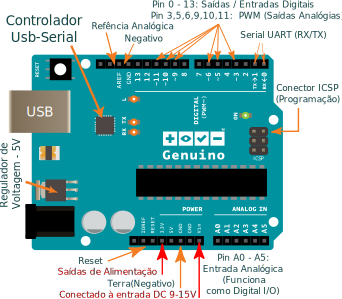
\includegraphics[width=0.8\linewidth]{Imagens/Cap_2/arduino}
\par\end{centering}
\caption[Placa Arduino ]{Placa Arduino (traduzido e adaptado de\cite{url:arduino:bord}) \label{fig:arduino}}
\end{figure}


\subsubsection{Características de Hardware}

O Arduino pode ser encontrado em várias versões, a maioria dos placas
são baseadas no microcontrolador Atmel AVR de 8 bits. A primeira placa
foi baseada na ATmega8 rodando a uma velocidade de clock de 16 MHz
com 8 KB de memória flash\cite{arduino:evans:2013}. Uma das placas
mais populares é o Arduino Uno\footnote{Arduino UNO (nos Estados Unidos) e Genuino UNO (fora dos Estados Unidos)},
que utilize o ATmega328p, com memória flash de 32KB e 2 KB de memória
RAM. Nos projetos mais exigentes, que requerem mais I/O e memória,
há o Arduino Mega 2560 com 256 KB de memória ou o Arduino Due\footnote{https://www.arduino.cc/en/Main/ArduinoBoardDue},
baseado no Atmel SAM3X8E ARM Cortex-M3, com 512KB de memória flash
e 96 KB de memória RAM.

As placas mais populares, em específico o Uno, têm 14 pinos digitais,
cada um dos quais podem ser definidos como entrada (input) ou saída
(output), e seis entradas analógicas. Além disso, seis dos pinos digitais
podem ser programados para proporcionar uma saída analógica PWM (Pulse
Width Modulation). Uma variedade de protocolos de comunicação estão
disponíveis, incluindo Serial, SPI (Serial Peripheral Interface),
e I2C (Inter-integrated Circuit Protocol). Na placa também é disponibilizada
uma entrada ICSP, que permite a programação do microcontrolador (que
é também realizada pela porta USB) e um botão de reset.

Placas especializadas chamadas \emph{Shields}, são usadas para expandir
as funcionalidade do Arduino. Estas podem ser empilhadas uma em cima
da outra para adicionar ainda mais funcionalidade, sendo esta, uma
das principais facilidades e fator de sucesso da plataforma Arduino.

\subsubsection{Características de Software}

Embora, muitas vezes o Arduino seja apresentado como uma linguagem,
na perspectiva de software, ele é na verdade um conjunto de bibliotecas
e APIs construídas em C/C++, que são baseadas nas APIs do projeto
Wiring.

A programação do Arduino é realizada por uma IDE (Integrated Development
Environment), escrita em Java e de código aberto\cite{arduino:source},
que fornece tudo que é necessário para a programação do Arduino, incluindo
uma série de programas de exemplo (sketches) que demonstram como conectá-lo
e se comunicar com alguns dispositivos comuns, como LEDs, LCDs, e
alguns sensores. 

A IDE do Arduino usa uma versão simplificada do C++\cite{arduino:ref},
tornando mais fácil aprender a programar e realizar interações com
o hardware. A estrutura básica de um programa para o Arduino é apresentado
na figura \ref{fig:arduino-1}. Programas escritos usando a IDE do
Arduino são chamados de sketches.

\begin{figure}[h]
\begin{centering}
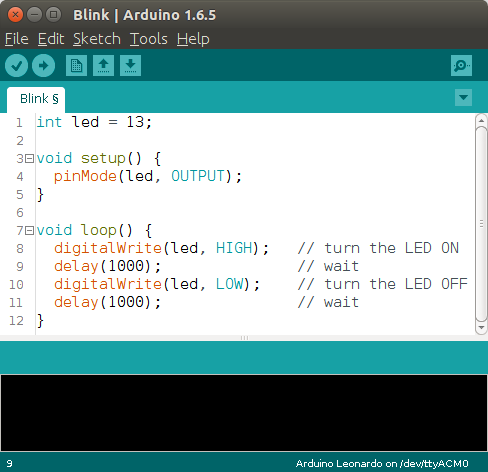
\includegraphics[width=0.6\linewidth]{Imagens/Cap_2/arduinoide_sketch}
\par\end{centering}
\caption{IDE do Arduino \label{fig:arduino-1}}
\end{figure}


\subsection{Raspberry Pi\label{subsec:Raspberry-Pi}}

O Raspberry Pi\cite{url:raspberry} é um mini PC de baixo custo, do
tamanho de um cartão de crédito, que possui recursos consideráveis
de processamento e memória. Ele foi desenvolvido no Reino Unido, com
intuito de fomentar a educação para adultos e crianças e logo se destacou
na comunidade de desenvolvedores antes mesmo do seu lançamento oficial
em junho de 2012.

O equipamento usa como seu Sistema Operacional (S.O), a distribuição
Raspbian Wheezy, que é baseada no Linux Debian. Porém, existem inúmeros
Sistemas Operacionais compatíveis\cite{raspberry:compatible}, incluindo
o Windows 10 IoT Core\cite{raspberry:compatible1}. 


\subsubsection{Características de Hardware}

Existem diferentes modelos, que contemplam diferentes características
técnicas. O Raspberry Pi 2 Model B (Figura \ref{fig:raspberry})\footnote{ref:https://www.raspberrypi.org/products/model-b-plus/},
possui um processador com arquitetura ARM, 900MHz de velocidade (permitindo
overclock) e 1GB de memória RAM. O processador é o BCM 2835, o mesmo
usado no iPhone 3g e Kindle 2. 

\begin{figure}[h]
\begin{centering}
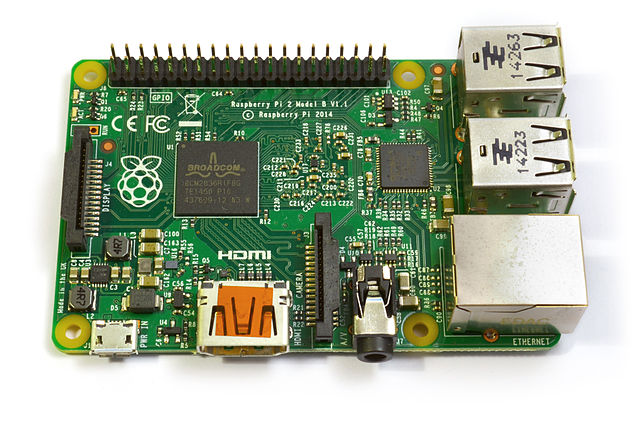
\includegraphics[width=0.8\linewidth]{Imagens/Cap_2/Raspberry_Pi_B}
\par\end{centering}
\caption{Raspberry Pi 2 - Model B \cite{img:raspberry} \label{fig:raspberry}}
\end{figure}


\paragraph*{Especificações:}
\begin{itemize}
\item SoC: Broadcom BCM2836 (CPU, GPU, DSP, SDRAM);
\item Processador: 900 MHz quad-core ARM Cortex A7 (ARMv7)
\item GPU: VideoCore IV @ 250 MHz / OpenGL ES 2.0 (24 GFLOFS);
\item Memória: 1GB MB (compartilhada com a GPU);
\item Saídas de Vídeo: 

\begin{itemize}
\item Vídeo Composto (PAL e NTSC) através de conector P2 com saída de áudio
integrada;
\item HDMI (ver 1.3 e 1.4);
\item Interface MIPI para ligar diretamente a painéis LCD.
\end{itemize}
\item Saídas de Áudio: Saída de áudio analógica através de conector P2 compartilhada
com o vídeo composto / HDMI;
\item Interfaces:

\begin{itemize}
\item 4 x portas USB 2.0;
\item 1 x MicroUSB (Alimentação);
\item 1 x Entrada MicroSD;
\item 1 x Ethernet (10/100Mbps);
\item 1 x GPIO (40 pinos) (General Purpose Input/Output).
\end{itemize}
\end{itemize}

\subsubsection{Características de Software}

Devido ao Raspberry Pi utilizar um S.O baseado em Linux e arquitetura
ARM, inúmeras linguagens de programação são suportadas\cite{raspberry:langs},
por exemplo, Java, JavaScript, PHP, Python, Ruby, etc. Bem como, é
possível executar servidores como Apache, Nginx e MySQL.

A distribuição oficial, Raspbian\cite{raspberry:os}, vem com suporte
nativo a Python e Java. A versão do Java instalada é a 'jdk-8-oracle-arm-vfp-hflt',
fornecida pela Oracle. É possível, contruir aplicações gráficas utilizando
\emph{JavaFX}\cite{raspberry:javafx}, tornando o Raspberry Pi, um
potencial equipamento para criação de inúmeras aplicações embarcadas.

Para controlar os pinos de GPIO em aplicações Java, existem várias
formas. Infelizmente a versão instalada não possui o suporte nativo
a este recurso (algo contraditório). Uma recente especificação, denomina
\emph{Device I/O}\cite{device-io:wiki}, foi projetada para acessar
os periféricos dos sistemas embarcados, permitindo acesso a recursos
como GPIO, I2C, SPI, UART, PWM, etc.

Para utilizar a API \emph{Device I/O}, é necessário instalar a versão
\emph{Java ME Embedded}\cite{device-io:wiki}, que conta com todos
componentes necessários. Porém, é possível utilizar API \emph{Device
I/O} com a versão do Java instalada por padrão no Raspberry Pi, necessitando,
neste caso, realizar a compilação da mesma.

Outra alternativa, é utilizar a biblioteca Pi4J\cite{raspberry:pi4j},
que permite realizar o acesso aos periféricos, utilizando uma API
Java totalmente orientada a objetos.


\subsection{BeagleBone}

A BeagleBone\cite{beagleboard} é outra plataforma na categoria de
mini PC, que se propõe a ser um computador de baixo custo, projetado
para fins educacionais. Ela foi projetado pela Texas Instruments,
e é totalmente open source, tanto em hardware quanto em software.

O equipamento usa como seu Sistema Operacional (S.O), a distribuição
Angstrom Linux, porém oferece suporte a outras versões do Linux, incluindo,
Debian, Ubuntu e Android.

\subsubsection{Características de Hardware}

Existem diferentes modelos, que contemplam diferentes características
técnicas. A BeagleBone Black (Figura \ref{fig:beaglebone}), possui
um processador AM3358BZCZ100, arquitetura ARM, 1Ghz de velocidade
e 512MB de memória RAM. Outros modelos podem chegar até 2GB de RAM.

Um dos diferencias em relação ao Raspberry Pi, é que ela possui uma
memória flash (eMMC) embutida de 4GB, onde é armazenado o Sistema
Operacional, o que permite um tempo carregamento do S.O menor (10s),
e maior confiabilidade do que o cartão MicroSD, utilizado no Raspberry
Pi.

Ao plugar a placa na porta USB do computador, ela é reconhecida como
um driver virtual de rede e pode ser acessada através do IP fixo\emph{
'http://192.168.7.2}'.

\begin{figure}[h]
\begin{centering}
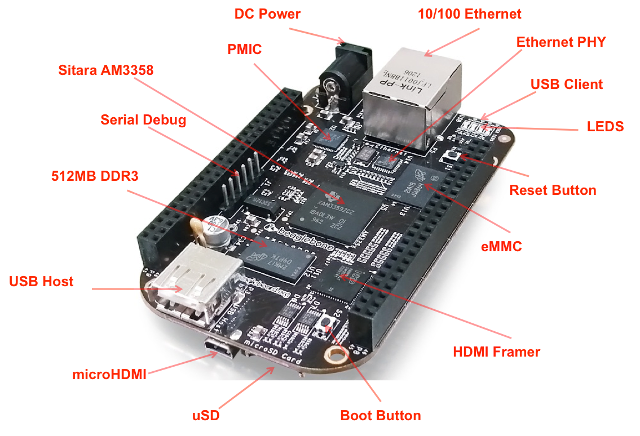
\includegraphics[width=1\linewidth]{Imagens/Cap_2/beaglebone}
\par\end{centering}
\caption{BeagleBone Black \cite{img:BeagleBone} \label{fig:beaglebone}}
\end{figure}


\paragraph*{Especificações:}
\begin{itemize}
\item Processador: TI Sitara™ AM3358 ARM\textregistered{} Cortex™-A8
\item GPU: Suporte a aceleração gráfica 3D;
\item Memória: 512MB DDR3;
\item Armazenamento: 4GB 8-bit eMMC Onboard Flash;
\item Saídas de Vídeo: Micro HDMI;
\item Saídas de Áudio: Micro HDMI;
\item Interfaces:

\begin{itemize}
\item 1 x portas USB 2.0;
\item 1 x MicroUSB (Alimentação e Comunicação);
\item 1 x Entrada MicroSD;
\item 1 x Ethernet;
\item 2 x GPIO (46 pinos) (General Purpose Input/Output).
\end{itemize}
\end{itemize}

\subsubsection{Características de Software}

Devido ao S.O ser baseado em Linux, as principais linguagens de programação
são suportadas. A distribuição oficial, Angstrom, vem como uma IDE
Web (baseada na Cloud9 IDE\footnote{https://c9.io/} e Node.JS), que
permite executar programas em JavaScript utilizando Node.js e a biblioteca
BoneScript. A biblioteca BoneScript, permite o acesso aos periféricos
e pinos de GPIO da placa, possui uma sintaxe simples, com algumas
funções similares ao Arduino.

O desenvolvimento de aplicações usando Java é suportado, porém, é
necessário instalar o Java JDK 1.8 SE para plataforma ARM. Infelizmente,
não está disponível até o momento, a versão \emph{Java ME Embedded
}para a BeagleBone\emph{, }que oferece suporte a API \emph{Device
I/O.} A alterativa, neste caso, é compilar a biblioteca. Apesar do
site do projeto \emph{Device I/O,} não mencionar a compatibilidade
com a esta placa, nos testes efetuados, a compilação foi realizada
com sucesso e o acesso aos pinos GPIO pode ser realizado através do
Java\emph{.}

Outra alternativa, é utilizar a biblioteca ``libbulldog''\cite{beagleboard:libbulldog},
que permite realizar o acesso aos periféricos, utilizando uma API
Java totalmente orientada a objetos.


\subsection{ESP8266}

O ESP8266\cite{url:esp8266:espressif}\cite{esp8266:datasheet} é
um SoC (System on a Chip), altamente integrado, projetado para as
necessidades de um mundo cada vez mais conectado. Ele oferece uma
solução completa e independente de rede Wi-Fi, permitindo rodar aplicações
embarcadas ou fornecer as funções de rede Wi-Fi para outros microcontroladores,
através de uma comunicação serial UART. O ESP8266 tem poderosas capacidades
de processamento e armazenamento que permitem que ele seja usado com
sensores e outros dispositivos através de suas interfaces de GPIO
(General Purpose Input/Output). Seu alto grau de integração ``\emph{on-chip}'',
permite a simplificação dos projetos de circuitos. Toda a solução,
incluindo o módulo, está concebido para ocupar uma área mínima de
PCB (Printed Circuit Board). Um dos principais atrativos e fatores
de sucesso, é seu baixíssimo custo\footnote{https://www.sparkfun.com/products/13678}
e a facilidade com que o mesmo pode ser integrado a demais soluções,
tornando-se uma das plataformas mais populares de desenvolvimento
nos últimos anos.

\subsubsection{Características de Hardware}

O ESP8266 (Figura \ref{fig:esp8266}b) foi desenvolvido pela \emph{Espressif
Systems}, como uma interface Serial (UART) para Wi-Fi, usando o microcontrolador
\emph{Tensilica Xtensa LX3} de 32-bits, com clock de 80MHz, 32KB RAM
(instrução) e 96KB RAM (dados). O núcleo da CPU é baseado no Xtensa\cite{esp8266:cadence},
da Cadence.

Os módulos ESP8266 são fornecidos numa ampla variedade de modelos,
com diferenças perceptíveis principalmente no que tange à quantidade
de pinos I/O disponíveis para acesso externo, e no tamanho do módulo.
Até o presente momento, \textquotedbl{}oficialmente\textquotedbl{}
existem módulos numerados de ESP-01 até ESP-12\cite{esp8266:modules}.
A Figura \ref{fig:esp8266}a, apresenta o módulo ESP-01.

\begin{figure}[h]
\begin{centering}
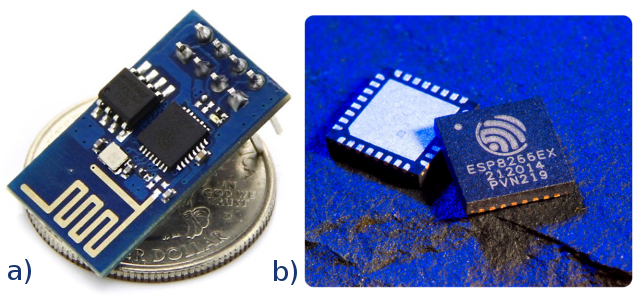
\includegraphics[width=0.8\linewidth]{Imagens/Cap_2/esp8266}
\par\end{centering}
\caption[Placa ESP8266]{Módulo ESP-01 (a), Chip ESP8266 (b), adaptado de \cite{url:esp8266:espressif}.
\label{fig:esp8266}}
\end{figure}


\paragraph*{Algumas características do módulo Wireless ESP8266:}
\begin{itemize}
\item Conexão à redes padrão 802.11 B/G/N;
\item CPU que opera em 80MHz, com possibilidade de operar em 160MHz;
\item Pilha TCP/IP integrada;
\item Tensão de operação : 3.3 V;
\item Tem conectores GPIO, barramentos I2C, SPI, UART, entrada ADC, saída
PWM e sensor interno de temperatura;
\item Suporte a memória Flash Externa - 512 KB até 16MB;
\item Modos de operação : Cliente, Access Point, Cliente+Access Point;
\item Modos de segurança Wireless : OPEN/WEP/WPA\_PSK/WPA2\_PSK/WPA\_WPA2\_PSK;
\item Suporta comunicação TCP e UDP, com até 5 conexões simultâneas.
\end{itemize}

\subsubsection{Características de Software}

A Espressif disponibiliza um SDK completo para trabalhar com o ESP8266\cite{esp8266:sdk}.
No SDK são disponibilizados recursos para suporte à SSL, JSON, e a
biblioteca lwIP\footnote{http://savannah.nongnu.org/projects/lwip/},
tornando esta uma solução bastante completa para criação de projetos
para a Internet das Coisas. A empresa possui um repositório no GitHub\cite{esp8266:source},
onde disponibiliza exemplos de código para firmwares com RTOS e comandos
AT. 

Alguns dos módulos vêm pré-carregados com um firmware que os transformam
em \textquotedbl{}Pontes Serial-WiFi\textquotedbl{}, permitindo serem
configurados e controlados por outros microcontroladores (ex.: Arduino).
Para realizar essa ponte, a interface serial dos módulos obedece a
uma tabela de comandos, que seguem o padrão AT, que podem variar de
acordo com a versão do firmware. 

Um dos firmwares mais populares é o NodeMCU\cite{esp8266:nodemcu},
que permite programar o módulo usando a linguagem de programação LUA,
tornando prático, por exemplo, a criação de um servidor Web com acionamento
de GPIOs. Existe também a possibilidade de programar o ESP8266 usando
JavaScript, através do firmware Espruino\cite{esp8266:espruino},
porém ainda em versão Beta.

Outra opção disponível, é programar o ESP8266 utilizando as APIs do
Arduino. A IDE do Arduino oferece suporte para o ESP8266, permitido
utilizá-lo como se fosse um Arduino. O núcleo ESP8266 para Arduino\cite{esp8266:arduino}
vem com bibliotecas para se comunicar através do Wi-Fi, usando servidores
TCP e UDP, configurar servidores HTTP, mDNS, e fazer atualizações
remotas. Permite também utilizar o sistema de arquivos em memória
flash ou cartões SD e realizar comunicação usando protocolos UART,
SPI e I2C.

\section{Rede de Sensores Sem Fio (RSSF)}

A combinação de sensoriamento, processamento e comunicação de interface,
oferta milhares de aplicações potenciais que é o conceito principal
de rede de sensores sem fio\cite{hill2003}. Os nós de sensores sem
fio são unidades auto-suficientes que consistem em uma fonte de energia,
capacidades de comunicação, poder de computação e um atuador ou sensor.
Eles podem se comunicar entre si, coletar dados do ambiente ao redor
ou se conectar a uma estação base externa ou centro de controle remoto\cite{olafsen2007}. 

Os recentes avanços tecnológicos em circuitos integrados de baixa
potência e comunicações sem fio, permitiram a criação de dispositivos
cada vez menores, com baixo consumo de energia e com baixo custo,
tonando-se soluções eficientes para uso em aplicações de sensoriamento
remoto. A combinação desses fatores melhorou a viabilidade de utilizar
uma rede de sensores composta por um grande número de sensores inteligentes,
permitindo a coleta, tratamento, análise e disseminação de informações
valiosas\cite{akyildiz2002}.

RSSFs em geral caracterizam-se por possuir uma alta densidade de nós.
Vários sensores monitoram o mesmo fenômeno, gerando dados redundantes
e, muitas vezes, fornecendo à aplicação um nível de qualidade maior
do que o necessário. Como a maior fonte de consumo de energia nos
sensores é a transmissão de dados, grande parte dos esforços de pesquisa
em RSSFs visa propor soluções para obter e rotear os dados de forma
eficiente em energia, a fim de estender o tempo de vida global da
rede. Por um lado, há propostas cujo enfoque é minimizar o número
de transmissões e/ou o tamanho das mensagens, realizando o roteamento
eficiente em energia\cite{heinzelman2000,intanagonwiwat2000}. Por
outro lado, pesquisas recentes\cite{perillo2003:1,perillo2003:2},
mostram que, em vez de fornecer uma redundância de dados desnecessária
para a aplicação, a alta densidade de nós pode ser aproveitada para
obter significativa economia de energia. Vários métodos podem ser
empregados a fim de se obter essa economia. 

A seguir estão algumas propriedades de redes de sensores sem fio:
\begin{itemize}
\item \textbf{Auto-organização:} Os nós de sensores podem criar automaticamente
a rede e a posição dos nós não precisam ser pré-determinada. Uma rede
de sensores auto-organizáveis não tem nenhuma necessidade de se ligar
a uma rede estabelecida.
\item \textbf{Comunicação de curto alcance e encaminhamento multi-salto:}
Comunicação multi-salto em redes de sensores sem fio é esperada para
consumir menos energia do que a comunicação tradicional de salto único.
Como sabemos, a potência de transmissão requerida aumenta com a distância
entre o transmissor e o receptor. Consequentemente, muitos pequenos
saltos requerem menos energia do que um longo salto.
\item \textbf{Cooperação entre nós:} Por causa dos recursos limitados dos
nós, papéis diferentes são atribuídos para nós na rede para alcançar
uma rede de baixa potência.
\item \textbf{Topologia Dinâmica:} Na rede de sensores sem fio, nós podem
falhar e ficar \emph{off-line}\footnote{fora de operação} ou novos
nós podem ser adicionados na rede. Assim, a topologia da rede opera
de forma dinâmica.
\item \textbf{Recursos energéticos limitados, poder computacional e memória:}
Uma vez que uma rede de sensores sem fio é composta por pequenos dispositivos,
a rede sofre com limitações de recursos, por exemplo energia, poder
computacional e memória.
\end{itemize}
É geralmente reconhecido que os sensores e redes de sensores serão
uma parte significativa da IoT \cite{Luckenbach2005}. Os sensores
podem monitorar o mundo físico por detectar e medir diferentes tipos
de informações ambientais. Ao alimentar aplicações adequadas com esse
tipo de informação através de vários tipos de objetos do mundo físico,
a Internet passaria de \textquotedbl{}computadores interligados\textquotedbl{}
para \textquotedbl{}as coisas interligadas.\textquotedbl{} Redes inteligentes
sensíveis ao contexto estão se aproximando rapidamente da posição
de sistemas de rede integrados, onde o desenvolvimento de minúsculos
sensores e atuadores pode perfeitamente realizar tais redes em grandes
ambientes de fábrica, redes para automóveis, residências, escritórios
inteligentes e serviços de apoio social, incluindo os alertas sísmicos,
monitoramento de pacientes e sensíveis ao contexto em situações de
emergência \cite{Luckenbach2005}.

\section{RFID}

O RFID - \emph{Radio Frequency Identification}, ou, em tradução livre,
Identificação por Radiofrequência, não é uma tecnologia nova, ela
teve seu início com o físico escocês Sir Robert Alexander Watson-Watt
em meados de 1937\cite{nemoto2012}. Esta tecnologia foi primeiramente
usada em sistemas de radares na Segunda Guerra Mundial para avisar
com antecedência a presença dos aviões aliados ou inimigos e que permaneceu
restrito somente para uso militar até os anos 70. C.M Roberts, em
\cite{Roberts2006}, descreve essa tecnologia como um ``sistema de
transação e identificação de dados por proximidade eletromagnética''.
O autor também afirma que o RFID é um melhoria sobre os códigos de
barras em termos de comunicação por proximidade não ótica.

Um sistema RFID consiste em leitores (também chamados de interrogadores)
e etiquetas (ou \emph{transponders}). Um sistema típico, tem alguns
leitores, estacionários ou móveis e muitas etiquetas que estão ligadas
a objetos, tais como livros, caixas de papelão, garrafas, etc\cite{Chawla2007}.
Um leitor se comunica com as etiquetas sem utilizar fios, dentro do
seu campo de atuação, e coleta informações sobre os objetos aos quais
as etiquetas estão associadas. Dependendo do seu princípio de funcionamento,
as etiquetas são classificados em três categorias: passivas, semi-passiva
e ativa.

A etiqueta passiva é a menos complexa e, portanto, a mais barata.
Não tem nenhuma fonte de alimentação interna, e usa o campo eletromagnético
transmitido por um leitor para alimentar seu circuito interno. Ela
não se baseia em um transmissor, mas em \textquotedbl{}retrodifusão\textquotedbl{}
para transmitir dados de volta para o leitor. A etiqueta semi-passiva
tem fonte de energia própria, mas nenhum transmissor, usando o mecanismo
de \textquotedbl{}retrodifusão. Uma etiqueta ativa, tem tanto fonte
de alimentação interna quando transmissor\cite{Chawla2007}.

A figura \ref{fig:rfid} ilustra o funcionamento do sistema RFID passivo
que consiste de uma etiqueta RFID e uma estação de base chamado \textquotedbl{}leitor
RFID\textquotedbl{}. Uma etiqueta passiva consiste em uma antena e
um circuito integrado de aplicação específica (ASIC), ambos com impedâncias
complexas. O chip obtém energia a partir do sinal de RF transmitido
pelo leitor RFID. A etiqueta envia dados de volta ao mudar a sua impedância
de entrada entre dois estados e modulando assim o sinal por \textquotedbl{}retrodifusão\textquotedbl{}. 

\begin{figure}[h]
\begin{centering}
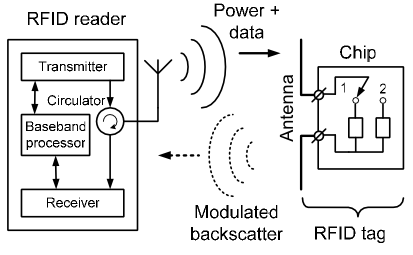
\includegraphics[width=0.5\linewidth]{Imagens/Cap_2/rfid}
\par\end{centering}
\caption{Visão geral do RFID passivo \cite{Chawla2007}\label{fig:rfid}}
\end{figure}

Atualmente, o RFID tem uma gama enorme de aplicabilidade, que vão
desde os conhecidos cartões de acesso residenciais por proximidade
até ao rastreamento em cadeias de produção, controle estacionamento
de veículos, gerenciamento de estoque, rastreamento de livros, prevenção
de roubos, etc\cite{Roberts2006}.

Esta tecnologia tem se difundido rapidamente pelo mundo, por sua facilidade
de uso e também pelo fato de dispensar a intervenção humana\cite{zhu2012review}.
no mundo dos negócios o RFID tem recebido grande expectativas com
previsão de crescimento de US\$ 4,96 bilhões em 2007 e US\$ 26,88
bilhões em 2017\cite{RFIDForecasts2007}.

O RFID possibilitou a inserção de inteligência nos objetos, trazendo
aos mesmos a capacidade de comunicarem-se de forma automática\cite{Khoo2010}.
Em \cite{Khoo2010}, o autor afirma que o RFID representa uma tecnologia
que possibilitou a convergência entre computação, comunicação e interação
através de redes sem fio, sensores e a grande rede de computadores.
Em complemento o autor afirma que esta tecnologia tem o potencial
que permite a máquina identificar objetos, compreender seus estados
e tomar medidas, se necessário. Ou seja, possibilitou aos objetos
do nosso cotidiano pensar e interagir. Todo esse desenvolvimento contribuiu
com a criação da Internet das Coisas (IoT), que permite a interação
inteligente entre objetos ao redor do mundo. As soluções categorizadas
de acordo com o domínio de redes de sensores e a tecnologia RFID têm
abordado de forma eficiente problemas relacionados a interoperabilidade,
escalabilidade, infraestrutura distribuída, interação espontânea\cite{Luckenbach2005}. 

\section{Tecnologias de Comunicação}

A Internet das Coisas necessita de tecnologias de comunicação na camada
física e do middleware para fornecer o controle dos dispositivos para
a camada das aplicações. Tipicamente, os meios físicos de comunicação
entre os dispositivos são baseados em três grupos diferentes: cabeamento
estruturado, a fiação existente, e sem fio\cite{ngo2007}.

Na maioria dos casos, os dispositivos usam a comunicação sem fio porque
os padrões de tecnologia sem fio estão em toda parte. A ampla disseminação
de redes sem fio em nossa vida diária está habilitado para os padrões
de comunicação, como Bluetooth, Zigbee, RFID, Wi-Fi e redes móveis
(3G/4G). Prevê-se uma combinação destas normas e tecnologias, afim
de construir ambientes inteligentes. Efetivamente, todas as tecnologias
sem fio que podem apoiar de alguma forma a transferência de dados
remotos, detecção e controle, são candidatas para inclusão no ambiente
de IoT.

\subsection{Tecnologias não IP}

\subsubsection{ZigBee}

ZigBee é uma tecnologia de rede sem fio desenvolvida pela ZigBee Alliance
para aplicações de baixa taxa de transmissão de dados e de curto alcance\cite{alliance2007}.
É uma especificação para um conjunto de rede, segurança, e camadas
de software de aplicações baseado no padrão IEEE 802.15.4 para redes
de área pessoal (PAN)\cite{hwang2012}.

A pilha do protocolo ZigBee é composta de quatro camadas principais:
a camada física (PHY), a camada de controle de acesso ao meio (MAC),
a camada de rede (NWK), e a camada de aplicação (APL). PHY e MAC de
ZigBee são definidos pela norma IEEE 802.15.4, enquanto o resto da
pilha é definido pela especificação ZigBee.

ZigBee é especialmente adequado para aplicações em sensores, incluindo
automação predial, interruptores de luz sem fio, medidores elétricos
e sistemas de gestão de tráfego. Em geral, é indicado para aplicações
em que altas taxas de transferências de dados não são requeridas.
A versão inicial do IEEE 802.15.4, em que ZigBee é baseado, atua nas
frequências de 868MHz, 915 MHz e 2,4 GHz, que estão disponíveis na
Europa, América do Norte e em todo o mundo, respectivamente. As taxas
de dados são 20 kb/s, 40kb/s, e 250kb/s, respectivamente\cite{gomez2010wireless}.

Os perfis de aplicações ZigBee mais importantes são o \emph{ZigBee
Home Automation Public Application Profile}\cite{alliance2007} e
do \emph{ZigBee Smart Energy} Profile\cite{alliance11smart}. As principais
áreas de aplicação para o perfil \emph{Home Automation} são de iluminação,
controle de temperatura, e segurança. O perfil \emph{Smart Energy}
lida com aplicações de gerenciamento de demanda de energia e de gestão
de carga para as redes de energia.

\subsubsection{Bluetooth}

Bluetooth, definido pela norma IEEE 802.15.1\cite{Bluetooth2004}
foi inventado pelo provedor de telecomunicações Ericsson em 1994,
e foi originalmente concebido como uma alternativa sem fios para a
comunicação por fios RS-232. É um protocolo projetado principalmente
para baixo consumo de energia com um curto alcance. Opera mundialmente
através de uma banda de frequência não licenciada (ISM) em 2.4 GHz
(2400-2483,5 MHz), com taxas de transmissão de 1 Mbit/s \cite{Haartsen:1998}.
A figura \ref{fig:bluetooth_stack} apresenta a pilha do protocolo
Bluetooth.

O sistema Bluetooth provê conexões ponto-a-ponto (apenas dois dispositivos
Bluetooth envolvidos), ou conexões ponto-multiponto. Nas conexões
ponto-multiponto, o canal é compartilhado entre alguns dispositivos
Bluetooth, formando uma piconet. Em uma piconet, um dos dispositivos
Bluetooth funciona como master (mestre), enquanto os demais funcionam
como slaves (escravos). O master controla o acesso dos dispositivos
slaves, determina o clock responsável pela sincronização, dentre outras
funções.

A figura \ref{fig:bluetooth_net} apresenta alguns exemplos de topologias
possíveis. Em \ref{fig:bluetooth_stack}a, tem-se uma piconet com
um único escravo. Em \ref{fig:bluetooth_stack}b, tem-se uma piconet
com múltiplos escravos. Em \ref{fig:bluetooth_stack}c, tem-se uma
possível configuração de uma scatternet\cite{BluetoothSpecv1}.

Bluetooth suporta ligações síncronas e assíncronas. O link síncrono
orientado a conexão (SCO) é usado principalmente para voz e eles são
transmitidos através de intervalos reservados. O link para conexão
assíncrona (ACL) é usado principalmente para transmissão de dados.
Ligação ACL pode utilizar as faixas restantes no canal. Ao contrário
de SCO, para garantir a integridade de dados, no ACL pacotes são retransmitidos.

Existem três diferentes classes de dispositivos Bluetooth. Cada classe
tem uma potência de transmissão diferente (daí um alcance de transmissão
diferente)\cite{BluetoothCore}:
\begin{itemize}
\item Classe 1: O alcance de comunicação é de 100 metros e a potência de
transmissão é de 100 mW (20 dBm)
\item Classe 2: O alcance de comunicação é de 50 metros e a potência de
transmissão é de 2,5 mW (4 dBm)
\item Classe 3: O alcance de comunicação é de 10 metros e a potência de
transmissão é de 1 mW (0 dBm)
\end{itemize}
\begin{figure}
\begin{centering}
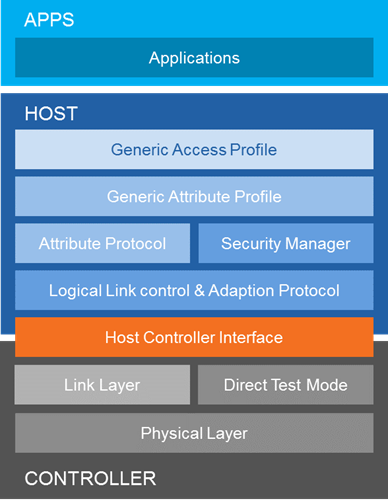
\includegraphics[width=0.4\linewidth]{Imagens/Cap_2/bluetooth_stack}
\par\end{centering}
\caption{Pilha do protocolo Bluetooth \cite{BluetoothCore} \label{fig:bluetooth_stack}}
\end{figure}

\begin{figure}
\begin{centering}
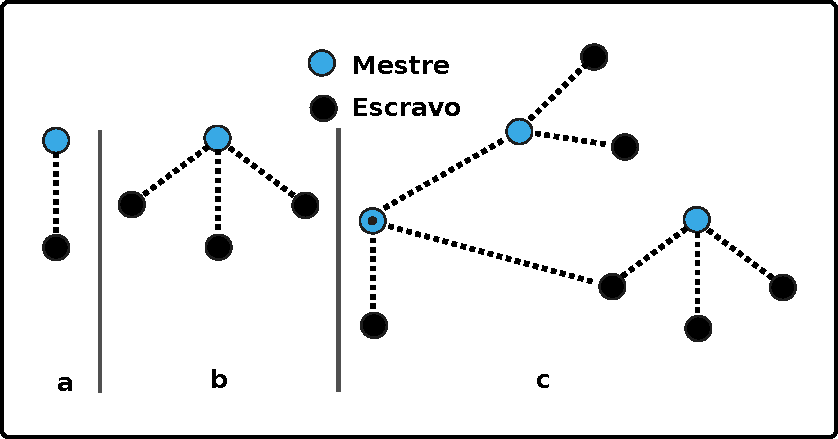
\includegraphics[width=0.6\linewidth]{Imagens/Cap_2/bluetooth_net}
\par\end{centering}
\caption[Topologias de redes Bluetooth]{Topologias de redes Bluetooth (traduzido de \cite{BluetoothSpecv1})
\label{fig:bluetooth_net}}
\end{figure}


\subsubsection{Bluetooth LE (Low Energy)}

Bluetooth \emph{Low Energy}, definido em \emph{Bluetooth Core Spec
4.0}\cite{bluetooth2010} e suas derivações 4.1 e 4.2, é um protocolo
sem fio operando na banda não licenciada de 2,4 GHz. Enquanto ela
opera na mesma faixa de frequência que outras tecnologias Bluetooth,
a sua operação nas camadas físicas (PHY) é incompatível, necessitando
de dispositivos com chipsets operem nos dois modos (Dual-mode)\cite{bluetooth2010}.
A camada PHY BT.LE usa \emph{Gaussian Frequency Shift Keying} (FSK)
com um deslocamento de 250 kHz. Ele transmite em um dos 40 canais
em 1 Mbit/s.

Segundo a Bluetooth SIG (Special Interest Group), o Bluetooth LE,
destaca-se como uma importante tecnologia para a Internet das Coisas:
\begin{quote}
Bluetooth 4.2 is an important update to the Bluetooth Core Specification
delivering exciting new features and benefits for Bluetooth Smart.
This will create significant advantages for developers and manufacturers,
while providing a better user experience for their customers. Bluetooth
4.2 makes Bluetooth Smart even smarter, faster and the ideal wireless
technology for the Internet of Things (IoT).\cite{bluetooth2010:site}
\end{quote}
Resumidamente as diferenças de aplicação entre as versões são destacadas
a seguir:
\begin{itemize}
\item Bluetooth BR/EDR (2.0/2.1): Estabelece uma distância relativamente
curta, conexão sem fio contínua, o que o torna ideal para os casos
de uso, tais como streaming de áudio. 
\item Bluetooth LE (4.0): Rajadas de conexão de rádio de longo alcance,
tornando-o ideal para a Internet das Coisas (IoT), aplicações que
não necessitam de conexão contínua, mas dependem de longa duração
da bateria.
\end{itemize}

\subsubsection{Z-WAVE }

Z-Wave é uma tecnologia desenvolvida pela Zensys e padronizado pela
Z-Wave Alliance, para automação em ambientes residenciais e comerciais.
Ela usa um rádio RF de baixa potência para aplicações de controle
remoto. O principal objetivo do Z-Wave é permitir transmissão de mensagens
curtas com consistência a partir de uma unidade de controle a um ou
mais nós na rede\cite{zwave:protocol2006}. Topologias de malha podem
ser formadas, no entanto, o esquema de endereçamento utilizado permite
um máximo de 232 nós na rede.

O rádio Z-Wave atua principalmente em 900 MHz (868 MHz na Europa e
908 MHz nos Estados Unidos) e 2,4 GHz, com taxas de dados entre 9,6
kbps e 40 kbps, e o alcance do sinal efetivo é de 30 metros em ambientes
fechados e é capaz de exceder a 100 metros ao ar livre, adequado para
aplicações com baixa taxa de transmissão de dados. À media que a distância
da comunicação aumenta, o mesmo ocorre com a complexidade do dispositivo,
o consumo de energia e os custos do sistema. Um característica do
chip de comunicação Z-Wave, é que ele pode ser colocado no estado
de dormência num longo período de tempo, gerando um baixo consumo
de energia, proporcionando uma maior duração da bateria para os dispositivos.

Embora atualmente o Z-Wave seja mais popular do que ZigBee para aplicações
de automação residencial, muitos especialistas do setor advertem
que Z-Wave sofre de algumas limitações fundamentais quando comparado
com ZigBee, já que Zigbee tem latência mais baixa (10 ms) e maior
taxa de transferência do que Z-Wave (latência de 100 ms). Embora o
Z-Wave tenha capacidade de redes mesh, este mecanismo não é tão robusto
quanto ZigBee. 

O Z-Wave define dois tipos de dispositivos: controladores e escravos.
Controladores fazem requisições ou enviam comandos para os escravos,
que respondem aos controladores ou executam os comandos recebidos.

\subsection{Tecnologias IP}

\subsubsection{Wi-Fi }

O objetivo do padrão IEEE 802.11\cite{ieee1997wireless} é fornecer
conectividade sem fio para dispositivos que requerem uma instalação
rápida, como computadores portáteis, PDAs ou dispositivos geralmente
móveis dentro de uma WLAN (Wireless Local Area Rede).

A rede IEEE 802.11 é uma especificação de rede local sem fio (WLAN).
No seu modo de banda baixa, IEEE 802.11 (b, g, n), pode transmitir
dados de 11 Mbps até 54Mbps e vai até 32 metros em ambientes fechados
e 95 metros ao ar livre\cite{Garroppo2011}. O padrão IEEE 802.11n
utiliza o dobro do espectro de frequência em comparação com 802.11a
ou 802.11g. No entanto, IEEE 802.11a, pode operar com uma taxa de
transmissão de até Gbps e pode exceder a faixa por mais de duas vezes
do que os padrões 'b' e 'g'. No modo de banda baixa, o Wi-Fi transmite
na faixa não licenciada (ISM) de 2,4 GHz, enquanto a banda alta transmitir
na faixa de 5 GHz.

Um novo padrão Wi-Fi, 802.11ah, na banda não licenciada de 900 MHz,
para aplicações de automação residencial e predial é esperado chegar
ao mercado ainda este ano\cite{wifi:zigbee}. Ele estará competindo
com outros protocolos já estabelecidos nesta banda, como o ZigBee.
WiFi AH visa apoiar uma gama de opções de taxa de transferência de
150Kbits com uma banda de 1MHz a até 40Mbits sobre uma banda de 8MHz.
Espera-se também cobrir distâncias de 50\% a mais do que outros produtos
802.11n.

O padrão 802.11af\cite{IEEE80211ah}, também chamado de Super Wi-Fi
ou White-Fi, emprega o espectro de frequências de TV não utilizadas,
entre 54 MHz e 790MHz, em intervalos muito longos (possivelmente vários
quilômetros). Pode oferecer rendimento razoável, talvez 24MB/s. Tem
aplicações semelhantes ao 802.11ah, também conhecido como Low Power
Wi-Fi, que irá fornecer largura de banda para sensores e monitores
em gadgets e aparelhos que irão juntar-se para criar a Internet das
Coisas.

\subsubsection{6LoWPAN}

6LoWPAN é uma definição de protocolo que descreve como utilizar IPv6
em cima de uma rede de baixo consumo de energia, baixa taxa de dados,
redes sem fio de área pessoal (WAN) e de baixo custo \cite{ZShelby2009}.
Os nós no 6LoWPAN são ligados em uma topologia de estrela ou de malha
e com suporte a taxas de transmissão de dados de 20 a 250kbps a uma
distância de cerca de dez metros. Projetado para enviar pacotes IPv6
sobre redes baseadas em IEEE~802.15.4 e implementar padrões IP abertos,
incluindo TCP, UDP, HTTP, COAP, MQTT e websockets.

Esta norma é desenvolvida para que os dispositivos de sensores sem
fio possam se conectar a redes IP existentes, como redes IPv4, sem
a necessidade de gateways de tradução ou proxy\cite{ZShelby2009}.
A camada física padrão 6LoWPAN é baseado em IEEE~802.15.4 (PHY) com
868/914 MHz ou 2,4 GHz rádio. A sub-camada MAC 6LoWPAN é totalmente
compatível com IEEE 802.15.4 MAC\cite{molisch2004ieee}. A estrutura
de pilha 6LoWPAN está ilustrada na figura \ref{fig:6LoWPAN}. Na pilha
de protocolos, a camada de ligação está dividida em sub-camada IEEE~802.15.4~MAC
e da camada de adaptação 6LoWPAN\cite{ZShelby2009}.

Em termos de roteamento da camada IP, 6LoWPAN suporta protocolos tais
como protocolos de roteamento de baixa potência e redes com perdas
(RPL)\cite{hui2012routing}, que atenua problemas, tais como estatísticas
de link não determinísticos e falta de visibilidade sobre topologia
física. 6LoWPAN suporta segurança apenas da camada de enlace através
de criptografia de 128 bits AES (Advanced Encryption Scheme). A coexistência
com outros dispositivos, tais como Wi-Fi, não é eficiente, por causa
da utilização de mesmo canal por todos os dispositivos. Alguns dispositivos
podem tirar vantagem ao usar o rádio de 2,4 GHz, mas, mesmo assim,
apenas três (15, 20 e 25) dos dezesseis canais vão evitar interferências\cite{angrisani2008experimental}.

\begin{figure}
\begin{centering}
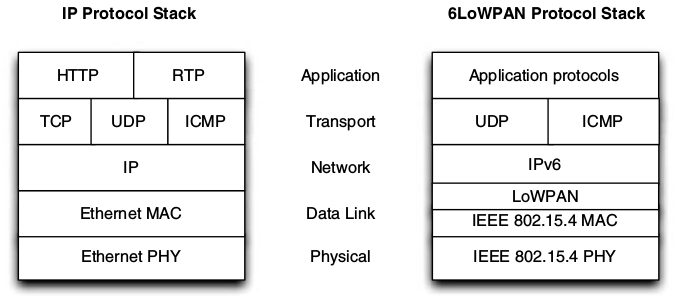
\includegraphics[width=1\linewidth]{Imagens/Cap_2/6LoWPAN_1}
\par\end{centering}
\caption{Pilhas do protocolo IP e 6LoWPAN \cite{ZShelby2009} \label{fig:6LoWPAN}}
\end{figure}


\section{Protocolos}

Nesta seção serão abordados os principais protocolos de comunicação
utilizados para a construção de aplicações IoT. Embora não exista
um protocolo definido para a Internet das Coisas, devido sua ampla
área de atuação e requisitos, várias propostas estão disponíveis na
literatura e no mercado. A seguir abordaremos com mais detalhes estes
protocolos.

\subsection{REST}

O REST - \emph{Representational State Transfer}, ou, em tradução livre,
Transferência de Estado Representativo, é uma técnica de engenharia
de software criado pelo Dr. Roy Fielding\cite{fielding2000architectural},
um dos autores da especificação do HTTP. Esta técnica foi criada para
trabalhar em sistemas distribuídos como o próprio WWW (Word Wide Web).
REST define como o design da aplicação se comportará: uma rede de
websites (um estado virtual), onde o usuário progride com uma aplicação
selecionando as ligações (transições do estado), tendo como resultado
a página seguinte (que representa o estado seguinte da aplicação)
que está sendo transferida ao usuário e apresentada para seu uso\cite{fielding2000architectural}.
Cada recurso possui um identificador único, chamado URI (Universal
Resource Indicators), que permite o acesso a tais recursos através
de uma URL. 

Um recurso é um mapeamento conceitual para um conjunto de entidades,
que segundo \cite{ibm:rest} “os clientes não acessam os recursos
diretamente, mas, em vez disso, uma representação do recurso através
de uma interface uniforme”. Tais recursos são apresentados, geralmente,
em XML ou JSON. A abstração chave da informação em REST é um recurso.
Qualquer informação que pode ser chamada pode ser um recurso: um documento
ou uma imagem, um serviço temporal (por exemplo, \textquotedbl{}o
tempo de hoje em Los Angeles\textquotedbl{}), uma coleção de outros
recursos, um objeto não-virtual (por exemplo, uma pessoa), e assim
por diante. Em outras palavras, qualquer conceito que pode ser o alvo
de referência de hipertexto de um autor deve caber dentro da definição
de um recurso. Um recurso é um mapeamento conceptual para um conjunto
de entidades \cite{fielding2000architectural}.

O sucesso desta técnica de engenharia de software, aplicado na arquitetura
cliente-servidor, é devido à possibilidade de separar do servidor,
a responsabilidade de montar a interface de apresentação de dados
aos clientes. Dessa forma as aplicações podem migrar para uma série
de plataformas, independente dos servidores. A separação de interesses
é o princípio por trás das restrições de cliente-servidor. Ao separar
as preocupações da interface de usuário das preocupações de armazenamento
de dados, podemos melhorar a portabilidade da interface do usuário
através de múltiplas plataformas e melhorar a escalabilidade, simplificando
os componentes do servidor. Talvez o mais importante para a Web, no
entanto, é que a separação permite que os componentes evoluam de forma
independente, suportando, assim, a exigência da Internet escalar de
vários domínios \cite{fielding2000architectural}.

Como já citado, os recursos acessados por uma aplicação REST são apresentados
em representações de dados, geralmente, identificado por um par, nome
e valor. A representação consiste em metadados que descrevem os dados
e, em certas ocasiões, metadados para descrever metadados (geralmente
com a finalidade de verificar a integridade da mensagem). Metadados
são na forma de pares nome-valor, onde o nome corresponde a um padrão
que define a estrutura e semântica do valor. As mensagens de resposta
podem incluir tanto metadados representativos quanto metadados de
recursos: informações sobre o recurso que não é específico para a
representação fornecida \cite{fielding2000architectural}.


\subsection{WebSocket}

O WebSocket é uma tecnologia que permite a comunicação entre cliente
e servidor de forma bidirecional (full-duplex), sobre um único soquete
TCP. Foi desenvolvido para clientes HTTP com suporte a HTML5, entretanto,
seu uso pode se estender a qualquer aplicação cliente-servidor\cite{Salim2013,Fette2011}. 

Devido ao fato de realizar um único pedido de conexão, e esta conexão
ser full-duplex, o servidor não precisa esperar uma requisição do
cliente para o envio de dados. Da mesma forma, o cliente pode enviar
informações a qualquer momento para o servidor. Isto causa uma redução
significativa da latência, comparando a um \emph{Polling} HTTP (requisições
de tempos em tempos). A comparação entre os mecanismo tradicional
usando \emph{Polling e usando }WebSocket, na figura \ref{fig:websocket}.

\begin{figure}[h]
\begin{centering}
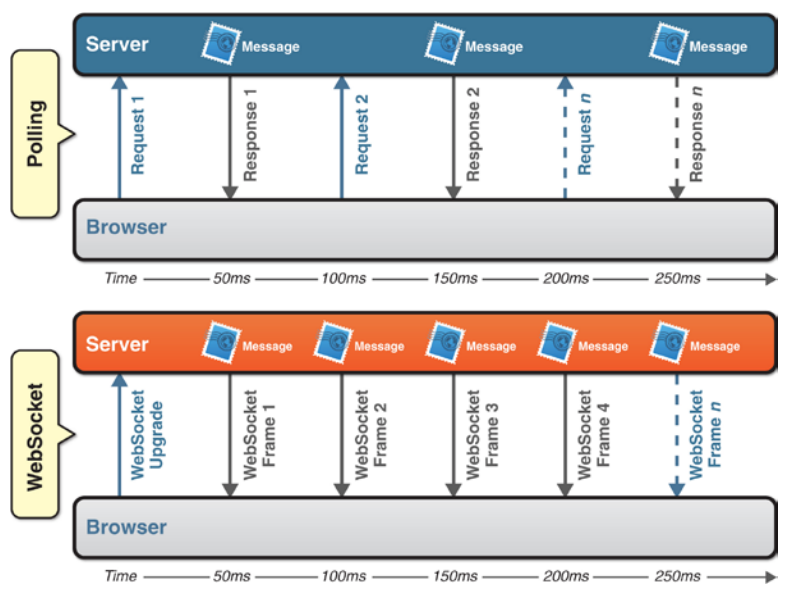
\includegraphics[width=1\linewidth]{Imagens/Cap_2/websocket_polling}
\par\end{centering}
\caption{Comparação de comunicação entre Pulling e WebSocket \cite{Salim2013}\label{fig:websocket}}
\end{figure}
 

O protocolo WebSocket é executado em duas etapas. A primeira é uma
mensagem de handshake (aperto de mão), onde tanto o cliente quanto
o servidor enviam suas respectivas informações. Após um handshake
bem sucedido, se inicia a transferência de dados. 

Segundo \cite{Fette2011}, os dados são transferidos em unidades conceituais
denominadas mensagens, onde estas não necessariamente representam
\emph{frames} da camada de rede. Neste caso um \emph{frame} possui
um tipo associado, e cada \emph{frame} pertence à mesma mensagem,
contendo o mesmo tipo de dados. Existem, de forma geral, três tipos
de dados específicos. São eles (1) os dados textuais, interpretados
em UTF-8; (2) dados binários, interpretados pela aplicação, e (3)
\emph{frames} de controle, responsáveis pelas sinalizações em nível
de protocolo, como informar que a conexão deve ser fechada. 

\subsection{CoAP}

O CoAP, acrônimo de Constrained Application Protocol, é um protocolo
da camada de aplicação leve e facilmente mapeável que tem como finalidade,
projetar um protocolo web genérico para necessidades especificas de
ambientes com restrições de recursos, tais como, memória, energia
ou processamento. Sua tecnologia objetiva reduzir, ao máximo possível,
o tamanho das mensagens utilizadas em sua comunicação\cite{Shelby2014}. 

O CoAP foi criado em 2010 por um grupo de trabalho do IETF (Internet
Engineering Task Force) chamado CoRE (Constrained RESTful Environments)\footnote{https://datatracker.ietf.org/wg/core/charter/},
com objetivo de prover um framework para aplicações que manipulam
recursos simples localizados em dispositivos interligados em redes
limitadas, incluindo desde aplicações que monitoram sensores de temperatura
e medidores de energia, até controle de atuadores como interruptores
ou trancas eletrônicas, e também aplicações que gerenciam os dispositivos
que compõem a rede\cite{coap:ietf2016}.

O CoAP baseia-se na abordagem de arquitetura REST, projetado para
o mapeamento fácil e sem estado (stateless) com o HTTP, e para proporcionar
interação M2M. A compatibilidade com HTTP é obtida através da manutenção
do mesmo modelo de interação, mas utilizando um subconjunto dos métodos
HTTP\cite{Shelby2014}.

Principais características definidas pela especificação:
\begin{itemize}
\item Protocolo Web que cumpre com os requerimentos M2M em ambientes restritos;
\item Troca de mensagens assíncrona;
\item Suporte à URI e Content-Type;
\item Capacidades simples de proxy e caching;
\item Mapeamento HTTP que permite que proxies possam prover acesso aos recursos
do CoAP via HTTP de maneira uniforme;
\item Interligação segura usando Datagram Transport Layer Security (DTLS);
\item Ligação em UDP com confiabilidade opcional suportando requisições
tanto unicast quanto multicast;
\item Suporte aos métodos GET, POST, PUT, DELETE.
\end{itemize}
A figura \ref{fig:coap} ilustra a arquitetura CoAP em uma perspectiva
de alto nível. Um dos objetivos do CoRE também consiste em adequar
a arquitetura REST, para ambientes restritos, composto por nós (ex.:
microcontroladores 8-bits com memória limitada) e redes (ex.: 6LoWPAN
e RFC4944\footnote{https://tools.ietf.org/html/rfc4944}). O CoAP
foi desenvolvido de acordo com esta arquitetura, logo pode ser considerado
como um protocolo RESTful\cite{Shelby2014}.

\begin{figure}[h]
\begin{centering}
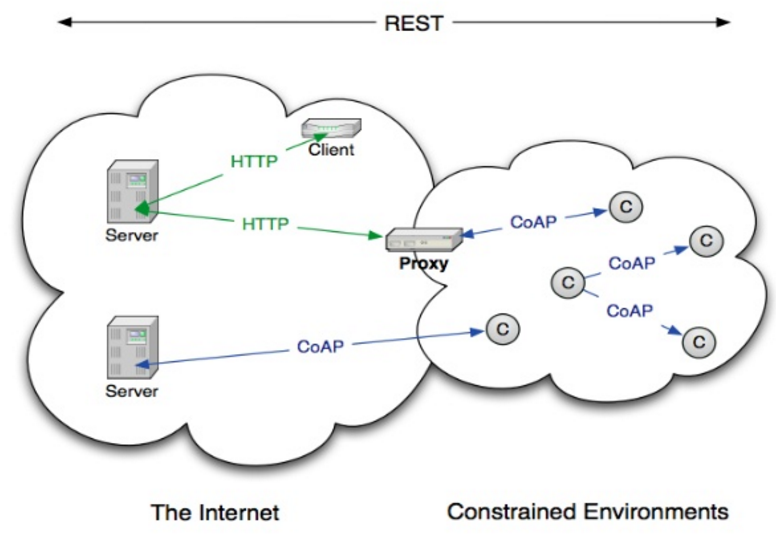
\includegraphics[width=0.8\linewidth]{Imagens/Cap_2/coap}
\par\end{centering}
\caption{Visão geral da arquitetura CoAP \cite{img:Shelby2014}\label{fig:coap}}
\end{figure}
 

\subsection{MQTT}

O protocolo MQTT (MQ Telemetry Transport)\cite{mqtt:spec}, é um protocolo
leve, baseado em mensagens seguindo o padrão \emph{publish/subscribe,}
executado sobre TCP/IP, usado para sensores remotos e controle de
dispositivos em ambientes com restrições como redes de baixa largura
de banda, pouco confiáveis ou comunicações intermitentes, principalmente
encontrados em contextos Machine to Machine (M2M) e Internet das Coisas
(IoT). O protocolo foi projetado para ser aberto, simples, leve e
fácil de implementar. Estas características o fazem ideal para ser
utilizando em ambientes e dispositivos com restrições de memória e
largura de banda, mas não limitados a estes.

O MQTT foi criado em meados de 1999 por Andy Stanford-Clark (IBM)
e Arlen Nipper (Eurotech). Atualmente, na versão 3.1.1, a especificação
do MQTT faz parte dos padrões OASIS\cite{mqtt:oasis}. O MQTT, na
sua essência, compartilha algumas características com o CoAP:
\begin{itemize}
\item São padrões abertos; 
\item São mais adequadas para ambientes com restrições;
\item Fornecem mecanismos para comunicação assíncrona; 
\item Executam sobre a pilha IP;
\item Têm uma série de implementações.
\end{itemize}

\subsubsection{Arquitetura}

O protocolo segue o padrão publish/subscribe (pub/sub), que é uma
alternativa para o modelo cliente-servidor tradicional, onde um cliente
se comunica diretamente com um ponto final. No entanto, o padrão publish/subscribe
desacopla um cliente, que está enviando uma mensagem particular (chamado
nesse caso de publisher) de outro cliente (ou mais), que está recebendo
a mensagem (chamado subscriber). Isto significa que o \emph{publisher}
e \emph{subscriber,} não sabem da existência do outro. Há um terceiro
componente, chamado de \emph{broker}, que é conhecido tanto pelo \emph{publisher}
quando pelo \emph{subscriber}, que filtra todas as mensagens recebidas
e distribui de forma adequada. 

As mensagens a serem transmitidas são publicadas para um endereço
(chamado de tópico), que assemelha-se a um sistema de arquivos, por
exemplo, \emph{casa/sala/temperatura}. Clientes por sua vez podem
se subscrever para vários tópicos, tornando-se assim capazes de receber
as mensagens que outros clientes publicam neste tópico. A figura \ref{fig:mqtt}
mostra uma rede de três clientes conectados com um broker central.
Quando o cliente ``\emph{MyTopicPublish}'', envia uma mensagem para
o tópico ``\emph{MyTopic}'', todos os interessados (\emph{subscriber}s)
recebem esta mensagem.

O MQTT não define o tipo dos dados contidos na mensagem (playload),
o \emph{publisher} pode enviar dados binários, dados textuais ou dados
estruturados como XML e JSON. Uma mensagem MQTT também tem mais alguns
atributos, que nós vamos discutir em detalhes a seguir.

\begin{figure}[h]
\begin{centering}
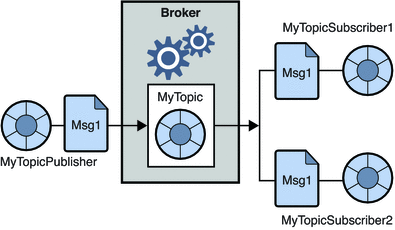
\includegraphics[width=0.8\linewidth]{Imagens/Cap_2/mqtt_broker}
\par\end{centering}
\caption{Padrão MQTT - Publish/Subscribe \cite{img:mqtt:oracle}\label{fig:mqtt}}
\end{figure}
 

\subsubsection{Formato da Mensagem}

As mensagens MQTT possuem um cabeçalho fixo composto de dois bytes,
campos opcionais de cabeçalhos variáveis e conteúdo da mensagem (playload).
Os cabeçalhos opcionais e playload dependem do tipo da mensagem transmitida.
A figura \ref{fig:mqtt-1} mostra o formato das mensagens MQTT.

\begin{figure}[h]
\begin{centering}
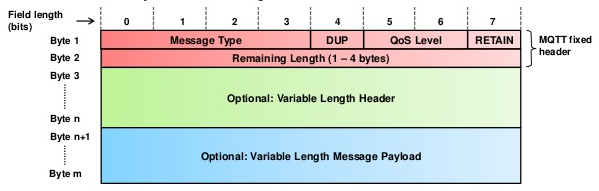
\includegraphics[width=1\linewidth]{Imagens/Cap_2/mqtt_message}
\par\end{centering}
\caption{Formato da mensagem MQTT \cite{img:mqtt:peter}\label{fig:mqtt-1}}
\end{figure}
 

No primeiro byte do cabeçalho fixo, os quatro primeiros bits representam
o tipo de mensagem, conforme a tabela \ref{tab:mqtt}, e os quatro
bits restantes são descritos a seguir:
\begin{itemize}
\item \textbf{Duplicate delivery (DUP)}: acrônimo relativo à entrega duplicada,
este marcador ocupa o bit 4 e é ativado quando o cliente ou o servidor
tentam reenviar mensagens do tipo \emph{PUBLISH, PUBREL, SUBSCRIBE}
ou \emph{UNSUBSCRIBE}, que tenham QoS > 0.
\item \textbf{Quality of Service (QoS)}: este marcador ocupa os bits 5 e
6, e indica o nível de garantia da entrega de uma mensagem \emph{PUBLISH}.
Os níveis de QoS são mostrados na tabela \ref{tab:mqtt_qos}.
\item \textbf{RETAIN}: quando um cliente envia uma mensagem \emph{PUBLISH}
ao servidor com este marcador ativado, ela deve ser retida no servidor
mesmo depois de ser entregue aos assinantes. No ocasião de uma nova
subscrição a um tópico, a última mensagem retida para este tópico
deve ser enviada para o novo assinante.
\end{itemize}
A largura restante do cabeçalho fixo (byte 2) é usada para representar
a quantidade de bytes remanescentes na mensagem. Incluindo dados do
cabeçalho variável e do payload. 

O cabeçalho variável é um componente presente em alguns tipos de mensagem
MQTT e está localizado entre o cabeçalho fixo e o payload.

O payload pode armazenar diferentes tipos de informações, tudo vai
depender do tipo da mensagem transmitida: CONNECT (irá conter ID do
cliente), SUBSCRIBE (contém tópicos que o cliente deseja subscrever)
ou SUBACK (lista de níveis de QoS garantidos pelo servidor).

\begin{table}[h]
\begin{centering}
\begin{tabular}{|c|c|c|}
\hline 
Mnemônico & Código & Descrição\tabularnewline
\hline 
\hline 
Reservado & 0 & Reservado\tabularnewline
\hline 
CONNECT & 1 & Requisição de conexão do cliente ao servidor\tabularnewline
\hline 
CONNACK & 2 & ACK de conexão\tabularnewline
\hline 
PUBLISH & 3 & Publicação de mensagem\tabularnewline
\hline 
PUBACK & 4 & ACK de publicação\tabularnewline
\hline 
PUBREC & 5 & Publicação recebida (garantia de entrega parte I)\tabularnewline
\hline 
PUBREL & 6 & Publicação liberada (garantia de entrega parte II)\tabularnewline
\hline 
PUBCOMP & 7 & Publicação completa (garantia de entrega parte III)\tabularnewline
\hline 
SUBSCRIBE & 8 & Requisição de subscrição do cliente\tabularnewline
\hline 
SUBACK & 9 & ACK de subscrição\tabularnewline
\hline 
UNSUBSCRIBE & 10 & Requisição de cancelamento de subscrição do cliente\tabularnewline
\hline 
UNSUBACK & 11 & ACK de cancelamento de subscrição\tabularnewline
\hline 
PINGREQ & 12 & Requisição PING\tabularnewline
\hline 
PINGRESP & 13 & Resposta PING\tabularnewline
\hline 
DISCONNECT & 14 & Cliente desconectando\tabularnewline
\hline 
Reservado & 15 & Reservado\tabularnewline
\hline 
\end{tabular}
\par\end{centering}
\caption{MQTT - Tipos de mensagem \cite{mqtt:spec}\label{tab:mqtt}}
\end{table}

\begin{table}[h]
\begin{centering}
\begin{tabular}{|c|c|c|c|}
\hline 
Valor QoS & Bit 2 & Bit 1 & Descrição\tabularnewline
\hline 
\hline 
0 & 0 & 0 & Até uma vez (Disparar e esquecer)\tabularnewline
\hline 
1 & 0 & 1 & Ao menos uma vez (Entrega com ACK)\tabularnewline
\hline 
2 & 1 & 0 & Entrega garantida\tabularnewline
\hline 
3 & 1 & 1 & Reservado\tabularnewline
\hline 
\end{tabular}
\par\end{centering}
\caption{MQTT - Níveis de QoS \cite{mqtt:spec}\label{tab:mqtt_qos}}
\end{table}


\section{Middleware\label{subsec:Fund_Middleware}}

É uma camada de software que lida com a execução e desenvolvimento
de aplicações distribuídas. Localiza-se entre o Sistema Operacional
(SO) e a aplicação abstraindo a complexidade e a heterogeneidade dos
elementos do sistema, além de coordenar como eles interagem entre
si\cite{mahmoud2004middleware}. Basicamente, utiliza mecanismos de
comunicação de baixo nível com a infraestrutura, para assim fornecer
uma comunicação de alto nível para as aplicações. Os middlewares podem
ser classificados em diversas categorias, e essas categorias estão
baseadas, por exemplo, na abstração fornecida para a programação da
comunicação (tuplas distribuídas, procedimentos, mensagens e objetos
distribuídos), em como as entidades se comunicam (cliente/servidor,
ponto-a-ponto e publish/subscribe), e no tipo de comunicação (síncrona,
assíncrona). 

\subsection{Componentes do Middleware de IoT}

Bandyopadhyay, S. et. al. realizou estudos sobre sistemas de middleware
que foram aplicados em sistemas baseados em IoT\cite{Bandyopadhyay2011}.
Eles classificam a funcionalidade necessária do middleware para gerenciar
interações com uma variedade de dispositivos em quatro componentes
funcionais, a saber: (1) protocolos de interface, (2) abstração de
dispositivos, (3) de controle central, detecção e gerenciamento de
contexto, e (4) abstração da aplicação (Figura \ref{fig:middleware_bandyopadhyay}).
A seguir, vamos explicar estes componentes em detalhes.

\begin{figure}[H]
\begin{centering}
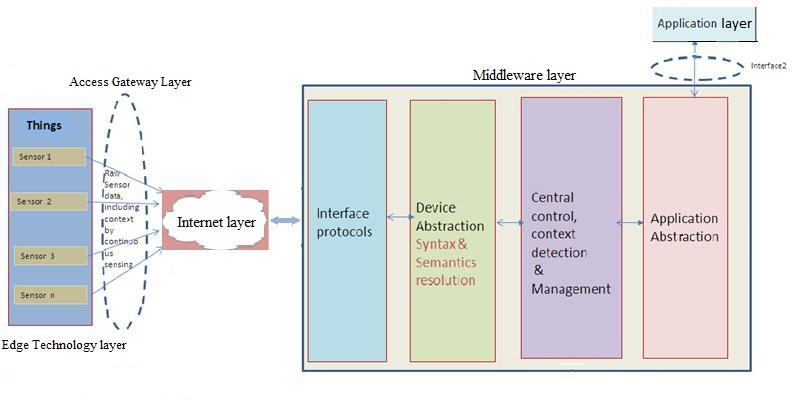
\includegraphics[width=1\linewidth]{Imagens/Cap_2/middleware_bandyopadhyay}
\par\end{centering}
\caption{Componente do Middleware de IoT \cite{Bandyopadhyay2011}\label{fig:middleware_bandyopadhyay}}
\end{figure}


\subsubsection{Protocolos de Interface}

Este componente é responsável pelo fornecimento da \emph{interoperabilidade
técnica}. Interoperabilidade no contexto de protocolos de interface
significa: \emph{a capacidade de dois sistemas interagirem utilizando
os mesmos protocolos de comunicaçã}o.

O componente de protocolo de interface define protocolos para a troca
de informações entre as diferentes redes que podem funcionar com base
em diferentes protocolos de comunicação, a fim de permitir a interoperabilidade
técnica. Este componente é responsável pelo tratamento de conectividade
básica na ligação física e de dados, rede, transporte, e às vezes
na camada de aplicação da pilha TCP / IP.

Para lidar com a heterogeneidade de dispositivos, podemos usar uma
camada de abstração (wrapper) para cada dispositivo, para traduzir
o protocolo suportado pelo dispositivo para um protocolo comum. Esta
abstração pode ser colocada no lado do dispositivo ou do lado de middleware.
Se quisermos ter uma interação direta com dispositivos, devemos colocar
a abstração no lado do middleware. Dispositivos normalmente têm capacidade
limitada de processamento computacional, pelo que esta seria uma razão
para implementar a abstração no lado do middleware.

\subsubsection{Abstração de dispositivos (Device Abstraction)}

Este componente é responsável pelo fornecimento de um formato abstrato
para facilitar a interação dos componentes de aplicação com os dispositivos.
Esta abstração fornece interoperabilidade sintáctica e semântica,
que são definidos pelo ETSI\cite{ETSI2006}, como segue:
\begin{itemize}
\item \emph{Interoperabilidade sintática} está associada com formatos de
dados. as mensagens transferido por protocolos de comunicação deve
ter uma sintaxe bem definida e formato de codificação, o qual pode
ser representado utilizando sintaxes de transferência de alto nível
tais como, JSON e XML.
\item A \emph{interoperabilidade semântica} é geralmente associada com o
significado do conteúdo da mensagem que é compreensível para todos
envolvidos na comunicação. Assim, a interoperabilidade a este nível,
significa que há um entendimento comum entre os componentes sobre
o significado do conteúdo (informação) que estão sendo trocadas entre
eles. Interoperabilidade semântica se baseia em modelos semânticos
que tende a ser de domínio específico. Por exemplo, uma forma de oferecer
interoperabilidade semântica em middlewares orientadas a serviços
(SOA)\cite{w3c:soa} é usando \emph{Devices Profile for Web Services}
(DPWS)\cite{driscoll2009devices}. Neste contexto, cada tipo de dispositivo
refere-se a um tipo de serviço diferenciado.
\end{itemize}

\subsubsection{Controle Central, Detecção de Contexto e Gerenciamento}

Contexto caracteriza a situação de uma entidade, que pode ser um lugar,
uma pessoa ou um objeto que é relevante para o usuário, aplicações
e suas interações \cite{Bandyopadhyay2011}. Este componente é responsável
por suportar a computação baseada em contexto (context-aware)\cite{schilit1994context},
que é um modelo computacional que levam em conta o contexto das entidades
que interagem com o sistema. Um middleware para sistemas baseados
em Internet das Coisas deve estar ciente de contexto para trabalhar
em ambientes inteligentes\cite{Bandyopadhyay2011}. Ambientes inteligentes
referem-se a um mundo físico que é ricamente e invisivelmente entrelaçada
com sensores, atuadores, monitores e elementos computacionais, encaixado
perfeitamente nos objetos do cotidiano de nossas vidas, e conectado
através de uma rede contínua. A consciência do contexto inclui duas
funcionalidades:
\begin{itemize}
\item A \emph{detecção de contexto}, que consiste em recolher os dados dos
recursos, e selecionar a informação que pode ter um impacto sobre
o cálculo. 
\item \emph{Processamento de contexto}, para usar as informações coletadas
para realizar uma tarefa ou tomar uma decisão.
\end{itemize}

\subsubsection{Abstração da Aplicação}

Este componente fornece uma interface de alto nível para aplicações
e os utilizadores finais, para interação com os dispositivos. Por
exemplo, esta interface pode ser uma interface REST ou pode ser implementada
com alguma linguagem baseado na consulta.

\subsection{Padronização\label{subsec:MiddlewarePadronizacao}}

Um único padrão para um middleware genérico de IoT, provavelmente
não vai existir, devido ao grande número e diferentes tipos de aplicações
e domínios envolvidos. No entanto, existem consideráveis esforços
para proporcionar um solução de middleware padronizado, específico
para um determinado domínio. Por exemplo, a visão proposta em \cite{Katasonov2008}
direciona-se no sentido de um middleware padronizado para o domínio
de aplicações de web semântica, enquanto que a solução fornecida em
\cite{hauswirth2006middleware}, tem como proposta oferecer uma abstração
para uma plataforma única para ambientes de redes de sensores. Para
ambientes inteligentes com uma infraestrutura fixa, como escritórios
inteligentes, a solução fornecida em \cite{roalter2010middleware}
pode perfeitamente se adequar às exigências requeridas para o middleware
neste contexto. Assim, é previsível que as plataformas de middleware
para IoT terão mais do que um padrão para permitir aplicações em diferentes
domínios. 

O conjunto de padrões estabelecidos para o desenvolvimento de plataformas
de middleware que venham atender os requisitos de todos os domínios
de aplicações, podem formar uma plataforma de normalização para pesquisas
e para indústria. Isto irá permitir a seleção do padrão desejado que
se encaixa em uma determinada aplicação, dentro de um domínio específico.


\section{Considerações Finais }

Este capítulo apresentou um resumo dos conceitos, que fundamentam
o desenvolvimento de middleware e firmware, bem como os protocolos
envolvidos na construção de projetos de IoT. 



\chapter{Trabalhos Relacionados}

Este capítulo tem por finalidade apresentar os principais trabalhos
de frameworks e middlewares para a área de Internet das Coisas, que
visam lidar com a grande heterogeneidade de dispositivos e protocolos,
fornecendo uma interface única e simples de comunicação.

Os trabalhos foram selecionados com base nas similaridades com a proposta
desse trabalho e com requisitos de código fonte e documentação disponível
para análises e testes. Alguns trabalhos foram abordados devido a
sua importância para área de pesquisa e fundamentos dos conceitos
iniciais de Internet das Coisas.

\section{OpenIoT}

O OpenIoT é um projeto co-financiado pelo FP7 (European Union's Research
and Innovation), para permitir \textquotedbl{}criar aplicações da
Internet das Coisas em grande escala de acordo com um modelo de entrega
de \emph{cloud computing}\textquotedbl{}\cite{kim2014openiot} O objetivo
principal é desenvolver uma infraestrutura de middleware para implementar
e integrar soluções da Internet das Coisas em um paradigma \textquotedbl{}Sensing
as a Service\textquotedbl{}. 

O projeto foca na convergência entre IoT e computação em nuvem, visando
assim fornecer uma “nuvem de coisas” (cloud of things, em Inglês).
Ele é apresentado como uma extensão para implementações de serviços
e recursos computacionais remotos, onde ele irá fornecer acesso a
recursos e capacidades dos dispositivos gerenciados pela sua plataforma.
OpenIoT abrange diversas áreas, a fim de constituir uma solução mais
completa:
\begin{itemize}
\item Middleware - para conexão de sensores e redes de sensores com a plataforma
(sensores ou fluxos de dados, a partir de dispositivos físicos ou
algoritmos de processamento apresentado como dispositivos virtuais);
\item Integração de Sensores - representado como sensores virtuais, utilizando
estruturas de middleware para redes de RFID / sensores sem fio (RSSF)
e Internet das coisas, fornecendo funcionalidades de linha de base
para o registro e de pesquisa, integração de sensores com o mínimo
esforço;
\item Ontologias, modelos semânticos e anotações - para representar informações
sobre objetos;
\item Computação em Nuvem, para fornecer disponibilidade com segurança e
privacidade;
\item Configuração flexível e implementação de algoritmos para a coleta
e filtragem de fluxos de informação;
\item Ferramentas visuais para gerenciar sensores e seus dados, para a composição
de serviços e para a visualização de dados com esforço mínimo de programação.
\end{itemize}
A arquitetura da OpenIoT (Figura \ref{fig:OpenIoT}) é composta por
três planos lógicos distintos: (1) Utilitário/Aplicação; (2) Plano
Virtualizado; e (3) Plano Físico. Tais planos, por sua vez, são compostos
por sete módulos principais, apresentados a seguir. 

\begin{figure}
\begin{centering}
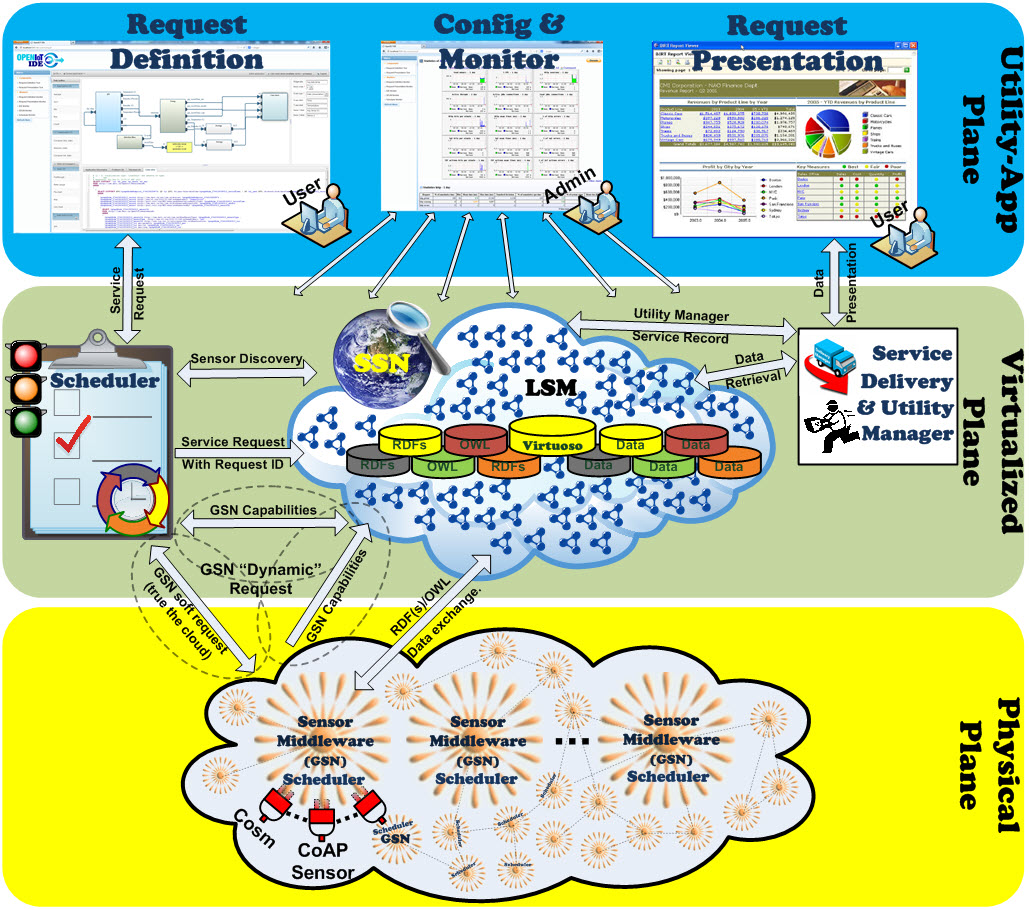
\includegraphics[width=1\linewidth]{Imagens/Cap_3/OpenIoT-Architecture}
\par\end{centering}
\caption{Arquitetura OpenIoT \cite{ZShelby2009} \label{fig:OpenIoT}}
\end{figure}


\paragraph*{Plano Utilitário / Aplicação }
\begin{itemize}
\item O componente \emph{Request Definition,} permite especificação, em
tempo de execução, de solicitações de serviços para a plataforma OpenIoT,
fornecendo uma interface Web 2.0. Compreende um conjunto de serviços
para a especificar e formular tais pedidos, ao mesmo tempo, submetê-los
ao agendador (\emph{Scheduler)} global.
\item O componente \emph{Request Presentation}, seleciona mashups a partir
de uma biblioteca apropriada, a fim de facilitar a apresentação de
um serviço em uma interface Web 2.0. Para visualizar estes serviços,
ele se comunica diretamente com o Service Delivery \& Utility Manager,
de modo a recuperar os dados relevantes.
\item A componente de configuração e monitoramento (\emph{Configuration
and Monitoring}), permite o gerenciamento e configuração de funcionalidades
sobre os sensores e os serviços que são implantados dentro da plataforma
OpenIoT. Além disso, permite ao usuário monitorar o estado dos diferentes
módulos implementados.
\end{itemize}

\paragraph*{Plano Virtualizado}
\begin{itemize}
\item O agendador (Scheduler) processa todas as solicitações de serviços
a partir da definição da solicitação (Request Definition) e garante
o seu acesso adequado aos recursos (por exemplo, fluxos de dados)
de que necessitam. 
\item A Nuvem de armazenamento de dados (LSM-Light), permite o armazenamento
de fluxos de dados provenientes do sensor, agindo assim como um banco
de dados em nuvem. O serviço armazena os metadados necessários para
o funcionamento da plataforma OpenIoT (dados funcionais). A implementação
do protótipo da plataforma OpenIoT usa o LSM Middleware, que foi re-projetado
com funcionalidades de dados push-pull e interfaces para permitir
streaming de processamento baseado em nuvem.
\item O serviço de entrega e gerenciador de utilitários (Service Delivery
\& Utility Manager), executa um duplo papel. Por um lado, ele combina
os fluxos de dados como indicado pelos fluxos de trabalho (workflows)
dentro do sistema OpenIoT a fim de entregar o serviço solicitado (com
a ajuda da consulta SPARQL fornecido pelo Scheduler), quer para a
solicitação de apresentação ou um aplicativo externo. Por outro lado,
esse componente atua como um mecanismo de medição de utilização dos
serviços, o que mantém o controle das métricas cada serviço individualmente.
\end{itemize}

\paragraph*{Plano Físico}
\begin{itemize}
\item O Sensor-Middleware (Extended Global Sensor Network, X-GSN), recolhe,
filtra, combina, e semanticamente anota fluxos de dados a partir de
sensores virtuais ou dispositivos físicos. Ele atua como um hub entre
a plataforma OpenIoT e o mundo físico. O Sensor-Middleware é implantado
com base em uma ou mais instâncias distribuídos (nós), que podem pertencer
a diferentes entidades administrativas. A implementação do protótipo
da plataforma OpenIoT usa o sensor-middleware GSN que foi ampliado
e chamado X-GSN.
\end{itemize}


\section{Eclipse IoT}

Eclipse IoT é um ecossistema de empresas e indivíduos que trabalham
em conjunto para estabelecer uma Internet das Coisas com base em tecnologias
abertas\cite{eclipse:iot}. O projeto fornece blocos de construção
que se apoiam em cima de padrões e protocolos abertos e fornecem serviços
e estruturas adicionais para gerenciamento de dispositivos, comunicação
e soluções verticais.

O primeiro projeto Eclipse IoT começou em novembro de 2012, hoje é
composto por subprojetos, focados no desenvolvimento de aplicações
para Internet das coisas e M2M. Em seguida é apresentado os principais
projetos mantidos de grupo.

\subsection{Padrões e Protocolos}
\begin{itemize}
\item \textbf{Paho}: prevê a implementação de clientes para o protocolo
de mensagens MQTT. O Paho, inclui clientes para Java, C, C++, Python,
JavaScript e outras implementações da da norma MQTT;
\item \textbf{Mosquitto}: implementação do servidor de MQTT;
\item \textbf{Californium}: é uma implementação Java do CoAP (Constrained
Application Protocol);
\item \textbf{OM2M}: é uma implementação do padrão OneM2M\cite{swetina2014toward}
(anteriormente chamado de padrão ETSI M2M). OM2M é um conjunto de
serviços Java e OSGi que implementam o padrão OneM2M;
\item \textbf{Wakaama}: é uma implementação do protocolo OMA Lightweight
M2M, para o dispositivos e gerenciamento de serviços. Wakaama é escrito
em C e projetado para ser portátil para sistemas compatíveis com POSIX.
\end{itemize}

\subsection{Frameworks e Serviços}
\begin{itemize}
\item \textbf{Kura}: é um conjunto de serviços Java e OSGi que implementam
os serviços comuns necessários para um gateway de Internet das Coisas,
tais como: (1) conexão de I/O com portas seriais, USB, Bluetooth,
GPS, (2) serviços de dados, (3) gerenciamento remoto, etc.
\item \textbf{Eclipse SCADA}: é um conjunto de serviços Java e OSGi para
a criação de sistemas de controle industrial que monitoram e controlam
processos industriais, como o chão de fábrica ou fazendas solares.
\item \textbf{Eclipse SmartHome}: é um conjunto de serviços para integração
de domótica em Java e OSGi. Este projeto fornece um ponto de acesso
uniforme para os diversos dispositivos e protocolos de automação residencial
diferentes.
\item \textbf{Ponte}: é um broker projetado para fazer a ponte entre protocolos
diferentes da Internet das Coisas (como MQTT e CoAP) e fornecer uma
API REST para esses padrões.
\item \textbf{Concierge}: é uma implementação do padrão OSGi, voltado para
pequenos dispositivos da Internet das Coisas.
\item \textbf{Krikkit}: é um projeto para definir regras para as mensagens
que passam através de um dispositivo de borda (edge device).
\item \textbf{Mihini}: é um framework baseado em Lua para a criação de aplicativos
para gateways IoT e M2M.
\end{itemize}
O Eclipse IoT é um projeto que vêm ganhando tração e incorporando
novos projetos\cite{eclipse:iot:projects}. Hoje conta com cerca de
110 colaboradores e é apoiados por empresas como IBM, Eurotech, 2lemetry,
Cisco, e outras.

\section{BUTLER}

BUTLER, acrônimo de uBiquitous, secUre inTernet-of-things with Location
and contExtawaReness, é um desenvolvido no âmbito do FP7, lançado
oficialmente em 2014, com o propósito de possibilitar o \textquotedbl{}desenvolvimento
de aplicações seguras e inteligentes de assistência pessoal graças
a um sistema pervasivo ciente de contexto e localização\textquotedbl{}\cite{BUTLER}.
BUTLER se concentra em:
\begin{itemize}
\item Melhorar / criar tecnologias para implementar uma Internet das Coisas
que seja segura (ligações seguras do físico para as camadas de aplicação),
pervasiva (aplicações abrangem diferentes cenários) e dependente do
contexto (ajusta às necessidades do usuário).
\item Integração / desenvolvimento de uma arquitetura em rede de dispositivos
inteligentes, onde os dispositivos podem ser categorizadas como SmartObjects
(sensores, atuadores, gateways), Smart Mobile (dispositivo pessoal
de usuário) e SmartServers (fornecedores de conteúdos e serviços).
\item Realização de estudos de caso para mostrar e ajudar a melhorar o projeto.
\end{itemize}
Foram definidos papéis de segurança no nível de aplicação, que refletem
os stakeholders participantes das interações em cada cenário. Os papéis
definidos no projeto são\cite{BUTLER:tec}:
\begin{itemize}
\item Usuário: entidade que ganha acesso a um recurso. Normalmente é um
humano, mas pode ser também uma aplicação;
\item Provedor de Recurso: entidade que provê um recurso e opcionalmente
o atualiza. Ele deve conferir o token de acesso apresentado para que
possa prover/atualizar um recurso;
\item Consumidor de Recurso: aplicação cliente recuperando e consumindo
recursos;
\item Servidor de Autorização: é a entidade que implementa a gestão de controle
de acesso. É responsável pela autenticação do usuário e autorização
do consumidor de recurso através da geração de um token de acesso,
relacionado ao recurso que se deseja acessar. Opcionalmente, pode
delegar a tarefa de autenticação para o servidor de autenticação;
\item Servidor de Autenticação: esta entidade pode ser utilizada pelo servidor
de autorização de modo a confiar em um protocolo de autenticação que
não é implementado nativamente no servidor de autorização. Isso significa
que o servidor de autenticação e o servidor de autorização precisarão
fazer a federação de identidades de usuários.
\end{itemize}
A arquitetura do projeto é baseada nas arquiteturas IoT-A e FI-WARE.
A figura \ref{fig:BUTLER}, apresenta as quatro principais camadas
definidas na arquitetura. 

\begin{figure}
\begin{centering}
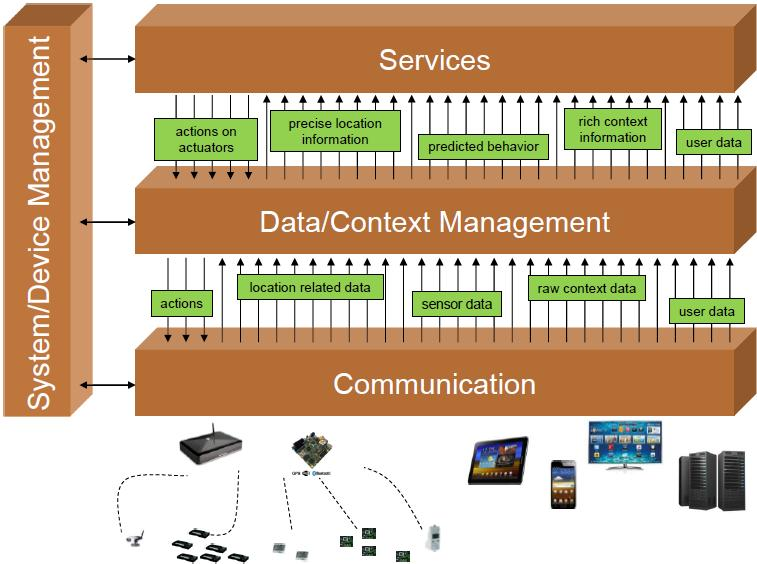
\includegraphics[width=1\linewidth]{Imagens/Cap_3/butler}
\par\end{centering}
\caption{Arquitetura proposta por BUTLER \cite{BUTLER}\label{fig:BUTLER}}
\end{figure}

\begin{itemize}
\item \textbf{Communications Layer:} lida com a infraestrutura de comunicação
fim-a-fim (com base em normas, tanto quanto possível), conectando
objetos inteligentes (SmartObjects), dispositivos móveis (SmartMobiles)
e plataformas de serviços (SmartObject Gateways e SmartServers). 
\item \textbf{Data/Context Management Layer}: especifica modelos de dados,
interfaces e procedimentos de coleta e processamento de dados. Com
informações de contexto, transforma os dados brutos em informações
ricas. 
\item \textbf{Services Layer}: define componentes e interfaces para a descrição,
descoberta, implantação e provisionamento de serviços sensíveis ao
contexto. 
\item \textbf{System/Device Management Layer:} gerencia e mantém objetos
inteligentes, serviços e outras entidades, como a configuração, gerenciamento
de desempenho, ou diagnósticos.
\end{itemize}

\section{LinkSmart (HYDRA)}

O LinkSmart (anteriormente chamado Hydra), tem como objetivo desenvolver
um middleware para sistemas embarcados inteligentes, baseado em uma
arquitetura orientada a serviços, implementável em redes novas ou
existentes, com ou sem fio, de dispositivos heterogêneos que operam
com recursos limitados em termos de energia, poder de computação e
uso da memória\cite{sarnovsky2007hydra}. A arquitetura LinkSmart
é baseada em três camadas: a camada física, a camada de middleware,
e a camada de aplicação. O middleware HYDRA, foi testado em três domínios,
tais como automação predial, área da saúde, e agricultura \cite{jahn2010energy}).
O usuário pode acessar os serviços oferecidos pelo HYDRA através de
uma interface inteligente móvel.

Middleware LinkSmart é um software inteligente que é colocado entre
as aplicações e o sistema operacional para lidar com várias tarefas
de uma forma eficiente em termos de custos. Este middleware fornece
uma interface de serviço web para interagir com todos os dispositivos
físicos, atuadores, sensores ou subsistemas, independentemente de
suas tecnologias de interface de rede, por exemplo, Bluetooth, RF,
ZigBee, RFID, Wi-Fi, etc.

Este middleware foi projetado para facilitar a interação com dispositivos,
abstraindo a partir das informações detalhadas sobre esses dispositivos
e suas redes. O LinkSmart considera cada dispositivo como um serviço,
e usa linguagens de ontologias, por exemplo, OWL, OWL-s e SAWSDL,
para definir as descrições semânticas desses dispositivos. Além disso,
ele fornece uma camada de serviço inteligente, que permite aos usuários
finais interagirem com esses dispositivos, sem lidar com a tecnologia
de comunicação que é suportado pelos dispositivos.


\section{TinyDB}

O middleware TinyDB\cite{madden2005tinydb} foi um dos primeiros projetos
a propor a ideia de abstração dispositivos. O TinyDB permite que usuários
finais interajam com os dispositivos sem saber sobre o detalhes da
especificação dispositivos, tais como os protocolos de comunicação
que são suportado por esses dispositivos.

O projeto fornece uma linguagem de domínio específico (DSL) para usuários
finais interagirem com os dispositivos. Sua DSL é uma linguagem de
consulta que suporta seleção, junção, projeção, e agregação, para
trabalhar com um ambiente de sensoriamento embarcado. Esta DSL permite
que um usuário final obtenha informações sobre o tempo, lugar, tipo
e método de amostragem em um ambiente de sensoriamento embarcado.
TinyDB suporta os seguintes tipos de consultas:
\begin{itemize}
\item Monitoring Queries: Ela pede o valor de um ou mais atributos periodicamente
e continuamente, tais como, informações sobre a temperatura.
\item Network Health Queries: Ele fornece informações sobre a própria rede.
Por exemplo, a seleção de nós vizinhos, com baixa vida útil de bateria.
\item Exploratory Query: Ela mostra o estado de um nó específico ou de um
conjunto de nós em um momento específico, tais como, por exemplo,
selecionar a temperatura do sensor através da sua identificação.
\item Actuation Query: Este tipo de consulta pode ser usada para pedir uma
ação física. Por exemplo, um usuário final pode querer ligar um ventilador
num ambiente em que a temperatura é superior a um limiar. 
\end{itemize}

\section{IoT@Work}

Este projeto é focado na automação industrial, levando em considerações
requisitos de comunicação e segurança. O projeto foi fundado pelo
FP7 e é liderado pelo Siemens AG\cite{IoTWork:site}\cite{rotondi2011project}.

O projeto tem como objetivo reduzir custos operacionais na configuração,
comissionamento, e manutenção da fabricação, principalmente diminuindo
o tempo para adaptação a mudanças no sistema.

Com base nos resultados dos projetos de investigação realizados, o
IoT@Work se concentra em melhorar a infraestrutura de comunicação
e middleware para construir a auto-gestão e redes resilientes e arquiteturas
de aplicativos orientados a serviços adaptados para ambientes de fábrica.

Os principais objetivos técnicos do projeto estão centrados em torno
dos seguintes objetivos:
\begin{itemize}
\item A dissociação entre a aplicação de automação e a configuração de rede
e operação, a fim de:

\begin{itemize}
\item Fornecer serviços avançados de comunicações que atendem demandas da
aplicação em termos de confiabilidade, comunicação em tempo real,
escalabilidade e segurança.
\item Reduzir os efeitos do processo de reconfiguração da aplicação sobre
o montante do planejamento manual necessária a nível da rede; 
\end{itemize}
\item Integrar mais auto-gestão em uma rede ``Plug\&Work'', a fim de:

\begin{itemize}
\item Ativar ``Plug\&Work'' em todos os níveis, especialmente durante
a fase de configuração das redes de automação industrial;
\item Levar em conta a semântica da aplicação e os fluxos de trabalho na
estruturação e otimização da operação da rede.
\end{itemize}
\item Garantir a resiliência e segurança em sistemas de automação em execução,
a fim de:

\begin{itemize}
\item Suporte a cenários de fabricação adaptáveis e ágeis, ao mesmo tempo
garantir e proteger a confiabilidade e a resiliência dos sistemas;
\item Integrar mecanismos de segurança fortes a nível arquitetônico e evitar
acesso não autorizado e interferências indesejadas com o processo
de produção.
\end{itemize}
\end{itemize}

\subsection{Arquitetura}

A arquitetura para este projeto foi desenvolvido em cooperação com
IoT-A\cite{rotondi2011project} e consiste de várias funções que são
implementadas por vários componentes, que são agrupados três camadas
principais, confirme a Figura \ref{fig:iot_work}.

\begin{figure}
\begin{centering}
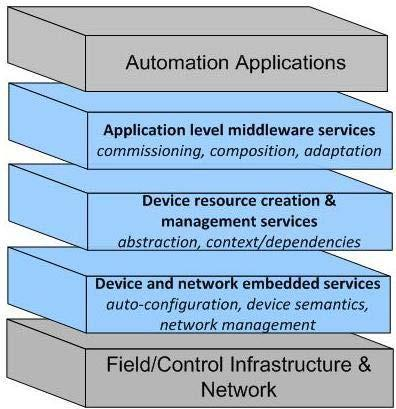
\includegraphics[width=0.5\linewidth]{Imagens/Cap_3/iot_work}
\par\end{centering}
\caption{Arquitetura IOT@Work - Camadas funcionais \cite{rotondi2011project}\label{fig:iot_work}}
\end{figure}

\textbf{Device and network embedded services}: realizar funções de
gestão, como a atribuição de identificadores, coletando semântica
de dispositivos e contexto e gestão de interfaces de comunicação.

\textbf{Device resource creation \& management services}: executar
agregação e gestão dos recursos e serviços incorporados e funções,
tais como o fornecimento de serviços de diretórios, abstração de redes
e monitoramento do sistema de baixo nível e de gestão de segurança.

\textbf{Application level middleware services}: oferece suporte para
aplicação por meio de serviços de middleware específicos para cenários
da Internet das Coisas. Nesta camada, a lógica do aplicativo é interpretada
através de configuração ou em tempo de execução e definição das interfaces
com os diferentes componentes IoT .

\subsection{Tecnologias Integradas}

Descrição da principais tecnologias envolvidas na construção da arquitetura
do IoT@Work\cite{IoTWork:site}.
\begin{itemize}
\item \textbf{Serviço de Diretório}: fornece um acesso unificado e baseado
em padrões para acesso às informações, escondendo a complexidade e
variedade de protocolos e formatos. Armazena informações que podem
ser atualizadas através da API RESTful.
\item \textbf{Auto-configuração de rede Ethernet em tempo real}: Atribuição
de endereço IP e URL, descoberta, e configuração em tempo real.
\item \textbf{Gerenciamento de Eventos (Serviço de Notificação de Evento}):
é um componente de middleware que atua como um conector flexível e
escalável entre fontes de eventos (ex.: \emph{Publishers}) e consumidores
de eventos (ex.: \emph{Subscribers}).
\item \textbf{Controle de Acesso}: O controle de acesso é apresentado em
dois níveis: (1) controle de acesso granular para as coisas, agentes,
aplicações, consumidores de dados, em todos os níveis e (2) controle
de acesso para garantir a confiabilidade da comunicação e estado da
configuração aos dispositivos embarcados.
\item \textbf{Processamento de Eventos Complexos (CEP)}: realiza processamento
inteligente de mensagem (análise de falhas, manutenção preditiva),
suporta a auto-gestão e permite a filtragem e combinação de eventos
para criar uma nova funcionalidade (usando regras inteligentes).
\item \textbf{Particionamento de Rede}: Ferramenta de gerenciamento de virtualização
de rede.
\end{itemize}

\section{Plataformas Comerciais}

O grande potencial esperado para Internet das Coisas\cite{GoldmanSachs2014,url:cisco:iot:2015,url:webintel:2015},
tem despertado a atenção de grandes empresas, que vem expandindo seus
serviços, muitos deles baseados em nuvem, para atender requisitos
de projetos de Internet das Coisas. A seguir, é apresentada uma lista
resumida das principais empresas de oferecem serviços para IoT.

\subsection{Google}

A Google vem investindo no cenário de IoT, e expandindo sua plataforma
em nuvem, \emph{Google Cloud Platform}, para atender os requisitos
de IoT. Os principais serviços incorporados na sua plataforma, são
destacados a seguir:
\begin{itemize}
\item Google Cloud Pub/Sub: É projetado para fornecer de mensagens assíncronas
muitos-para-muitos de maneira confiável entre aplicações.
\item Device Streaming: Oferece suporte para processamento, armazenamento
e análise de centenas de milhões de eventos.
\end{itemize}
A aquisição da empresa Nest em fevereiro de 2014, por cerca de 3,2
bilhões de dólares, vem mostrando o direcionamento da empresa para
áreas de computação embarcada e IoT. Outro projeto em desenvolvimento
é o Brillo, que tem como objetivo fornecer um sistema operacional
para dispositivos embarcados baseados em plataformas ARM, Intel x86,
and MIPS, focado em dispositivos com memória RAM a partir de 32MB.


\subsection{Oracle}

Oferece uma plataforma\cite{oracle:iot} baseada em nuvem, para conectar,
analisar, e integrar dispositivos, processos de negócios e aplicações.
As principais recursos oferecidos estão relacionados à virtualização
de dispositivos, comunicação bi-direcional, gerenciamento de metadados,
processamento de eventos e \emph{Big Data}. 

\subsection{Salesforce - IoT Cloud}

A plataforma oferecida pela Salesforce\cite{salesforce:iot}, é um
serviço baseado em nuvem, focado principalmente em processamento de
eventos complexos integrados com processos de negócio. O projeto denominado
Salesforce Thunder, é a peça central da plataforma, e é apresentado
pela empresa, como o motor de processamento de eventos mais rápido.

\subsection{IBM}

A plataforma ``IBM IoT Foundation''\cite{ibm:iot}, permite que
as organizações conectem dispositivos de forma fácil e segura, a partir
de chips à dispositivos inteligentes. Escalando através de serviços
baseados em nuvem, e usando análises ricas, a plataforma fornece às
organizações uma nova visão de inovação e transformação.

Outro projeto liderado pela empresa é o ``Watson Internet of Things'',
que tem o foco na inteligência computacional de cognição e inferência.

\subsection{Amazon IoT}

O AWS IoT\cite{amazom:iot} é uma plataforma que permite conectar
dispositivos aos serviços da AWS e a outros serviços. Permite interação,
processamento dos dados dos dispositivos e integração com aplicações,
mesmo quando eles estiverem off-line. A empresa oferece um SDK (AWS
IoT Device SDK), que permite que os dispositivos facilmente se conectem
à nuvem usando protocolos MQTT ou HTTP, suportando dispositivos como
Arduino e linguagens C e JavaScript.

\subsection{Microsoft}

A recente parceria entre Microsoft e Arduino\cite{microsoft:arduino},
demostra a aproximação da empresa na construção de projetos de IoT
e o apoio à projetos open source. A empresa possui projetos tanto
a área de sistemas embarcados, com o sistema operacional Windows 10
IoT Core, compatível com Raspberry Pi, quando para serviços em nuvem,
com o Azure IoT Suite\cite{microsoft:iot}.

\subsection{Intel}

A Intel é outra empresa que vem apostando fortemente no mercado de
IoT, contando com projetos para dispositivos embarcados e soluções
em nuvem. Na perspectiva de projetos cloud a empresa oferece o ``Intel\textregistered{}
IoT Platform''\cite{intel:iot}, com o objetivo de interconectar
dispositivos de forma segura e escalável, permitindo a análise e extração
de valor dos dados.

Na área de dispositivos embarcados a empresa oferece kits de desenvolvimento
que contam com a placa Galileo, com compatível e certificada pelo
Arduino\footnote{https://www.arduino.cc/en/ArduinoCertified/IntelGalileo},
e a placa Intel\textregistered{} Edison\footnote{https://software.intel.com/pt-br/iot/hardware/edison},
também compatível com Arduino e de fácil integração aos serviços Microsoft
Azure IoT Suite e Amazon AWS.

\subsection{Xynvely}

A plataforma Xively\cite{Xively:iot}, desenvolvida pela empresa LogMeIn,
utiliza serviços de nuvem para gerenciar dados providos por dispositivos.
A plataforma fornece uma API para envio de dados a partir dos sensores,
permitindo assim a visualização de dados históricos e provendo mecanismos
para disparar eventos com base nos dados gerados pelos sensores (os
chamados triggers). Na plataforma, os dados são organizados em feeds,
datapoints e datastreams.

\section{Considerações Finais}

\subsection{Análise das Plataformas Abertas}

Os projetos selecionados para análise tem como característica em comum
as capacidades de abstração de hardware, código fonte disponível,
e o fato de terem sido desenvolvidos recentemente. O TinyDB e as plataformas
comerciais não serão incluídos nessa análise.
\begin{itemize}
\item Disponibilidade de documentação e código fonte: 

\begin{itemize}
\item O(s) projeto(s): BUTLER, IoT@Work e LinkSmart, são projetos que apesar
de terem código fonte disponível, não possuem informações de como
realizar o processo de compilação, ou mesmo, não é disponibilizado
o código de todos os componentes, impossibilitando a análise e testes
aprofundados.
\item O(s) projeto(s): OpenIoT e Eclipse IoT, possuem boa quantidade de
documentação, guias de instalação e o código de todos componentes
são acessíveis (github). Porém os dois possuem um processo de ``setup''
relativamente complexo.
\end{itemize}
\item Abstração do Hardware:

\begin{itemize}
\item Todos os projetos avaliados atendem bem a este requisito. No Eclipse
IoT ele é implementado pelo sub-projeto chamado Leshan\footnote{http://www.eclipse.org/leshan/},
focado na comunicação M2M e CoAP.
\end{itemize}
\item Integração com plataformas de hardware mencionadas na seção \ref{sec:Plataformas-de-Desenvolvimento}:

\begin{itemize}
\item O(s) projeto(s): Eclipse IoT, é um dos poucos a dar ênfase nessas
plataformas, porém, devido o requisito anterior, existem algumas lacunas
a serem abordadas. 
\end{itemize}
\item Complexidade no desenvolvimento de projetos:

\begin{itemize}
\item O(s) projeto(s): BUTLER, IoT@Work e LinkSmart, não puderam ser avaliados
conforme a complexidade do desenvolvimento, pois não possuem instaladores,
nem foi possível a compilação a partir dos códigos fonte.
\item O(s) projeto(s): Eclipse IoT e OpenIoT, devido à grande quantidade
de componentes, possuem um processo de compilação complexo e demoraram
para serem configurados. O Eclipse IoT é o mais favorável neste quesito,
apesar de termos encontrado algumas falhas nos testes iniciais.
\end{itemize}
\item Ferramentas para auxílio na construção das aplicações embarcadas (firmware):

\begin{itemize}
\item O(s) projeto(s): Eclipse IoT, possui subprojetos WAKAAMA e Leshan,
que possuem recursos e bibliotecas em C para desenvolvimento para
microcontroladores, porém o mesmo, necessita de 100kb de flash e 10kb
de RAM. O sub-projeto Eclipse Paho, disponibiliza bibliotecas compatíveis
com o Arduino para comunicação usando MQTT.
\end{itemize}
\item Ferramentas de visualização e interface com os dispositivos:

\begin{itemize}
\item O(s) projeto(s): OpenIoT, oferece interfaces avançadas para configuração
de dispositivos, composição e orquestração de serviços. O projeto
Eclipse IoT, mais especificamente o sub-projeto Leshan, possuí alguns
recursos simples para interação com os dispositivos.
\end{itemize}
\item Abstração de comunicações: Bluetooth, USB, Ethernet, WiFi:

\begin{itemize}
\item A maioria dos projetos estão voltados para comunicação usando protocolo
IP, com exceção do Eclipse IoT (subprojeto Kura), que possui implementações
para comunicação USB e Bluetooth.
\end{itemize}
\item Auxílio na construção de aplicações Web:

\begin{itemize}
\item O(s) projeto(s): Eclipse IoT, possuem implementações de clientes MQTT
em JavaScript no sub-projeto Paho, porém não possui nenhuma implementação
para abstração de dispositivos na camada Web em JavaScript. 
\end{itemize}
\item Auxílio na construção de aplicações Mobile (Android):

\begin{itemize}
\item O(s) projeto(s): Eclipse IoT, possui apenas implementação para clientes
MQTT, e no projeto OpenIoT, foram encontradas apenas interfaces gráficas
de visualização de dispositivos, nenhuma ferramenta específica para
desenvolvimento.
\end{itemize}
\end{itemize}


\subsection{Análise das Plataformas Comerciais}

Não é objetivo desta dissertação o aprofundamento na análise de plataformas
proprietárias, limitando-se apenas a algumas considerações.

As plataformas proprietárias oferecem um requisito importante para
projetos de IoT, principalmente, quando os mesmos necessitarem trabalhar
com uma grande quantidade de dispositivos, que está relacionado à
escalabilidade. A maioria das soluções abordadas neste trabalho, são
de empresas que oferecem outros serviços relacionados a \emph{cloud
computing}, que por natureza, necessitam de um infraestrutura altamente
escalável. Por outro lado, essas plataformas comerciais precisam estar
baseadas em protocolos abertos para sua ampla difusão e penetração
do mercado de IoT.

As empresas que mais se destacam no desenvolvimento e apoio de padrões
abertos são a Amazon AWS, Microsoft (contrariando as expectativas)
e Intel. Estas empresas, também oferecem suporte para os hardwares
abertos (como Arduino), e biliotecas para a integração com seus serviços
em núvem.

A Google, na sua plataforma, parece estar direcionada a usar seus
próprios padrões\footnote{http://venturebeat.com/2015/05/28/google-announces-brillo-os-for-the-internet-of-things/}\footnote{https://cloud.google.com/pubsub/docs},
e até o momento não oferece suporte ao MQTT. 



\chapter{Arquitetura Proposta\label{sec:Arquitetura}}

Este capítulo apresenta a arquitetura empregada na construção do OpenDevice.
A arquitetura proposta será apresentada em uma visão top-down (de
cima para baixo), onde partiremos de uma abordagem em alto nível até
um nível mais baixo, apresentando detalhes de implementação. Na primeira
seção (\ref{sec:VisaoGeral}), será apresentado a visão geral da arquitetura,
permitindo o entendimento de suas camadas, modelos de comunicação,
requisitos e extensibilidade. Na seção \ref{subsec:Arquitetura-Detalhada},
será apresentada uma visão mais detalhada dos componentes da arquitetura,
detalhando os módulos que compõe a arquitetura e responsabilidades.
As seções \ref{sec:GerenciamentoDispositivos}, \ref{sec:ModeloEventos}
\ref{sec:APIComandos} e \ref{sec:Armazenamento} apresentam os detalhes
de como é realizada a abstração dos dispositivos e nas seções \ref{subsec:ConexoesServidores}
e \ref{subsec:ConexoesCliente}, são apresentados os recursos que
permitem que as aplicações clientes se comuniquem com os dispositivos
físicos, utilizando por exemplo o protocolo MQTT. A seção \ref{sec:MecanismoExtensao},
apresenta os mecanismos de extensibilidade que a plataforma oferece,
em complemento ao framework de conexões que é apresentado na seção
\ref{subsec:Framework-de-Conexoes}. Na seção \ref{subsec:Arquitetura-do-Firmware}
são apresentado os detalhes da arquitetura utilizada na construção
do firmware, um componente importante que permite a criação de dispositivos
(sensores e atuadores) para internet das coisas, utilizando componentes
de baixo custo, de maneira simplificada e extensível, e com suporte
a várias tecnologias de comunicação. Um protocolo simples e fácil
de ser implementado é proposto na seção \ref{subsec:Protocolo} ,
para permitir a integração entre software e hardware com baixo poder
de processamento. 


\section{Visão Geral\label{sec:VisaoGeral}}

O OpenDevice é uma plataforma aberta (\emph{open source}) que tem
como objetivo fornecer uma solução completa para a criação de projetos
baseados na Internet das Coisas. Suas ferramentas abrangem todas as
plataformas envolvidas no ecossistema de IoT: (1) Hardware, (2) Desktop,
(3) Cloud, (4) Mobile, (5) Web, promovendo uma infraestrutura de comunicação
entre todas essas camadas, bem como serviços de: (1) Armazenamento,
(2) Controle, (3) Configuração, (4) Visualização. A base da arquitetura
foi construída usando a linguagem de programação Java, e por ser multi-plataforma,
vários componentes podem ser reutilizados em várias plataformas. Devido
à limitação de recursos de processamento e memória de alguns dispositivos
embarcados alvos desse projeto, como no caso dos microcontroladores
AVR/Arduino, um protocolo de nível de aplicação foi elaborado, implementado
e disponibilizado através de bibliotecas em C/C++. Hardwares mais
robustos, como no caso do Raspberry, Beaglebone ou outro dispositivo
que tenha uma implementação da JVM disponível, podem executar as implementações
em Java diretamente. O OpenDevice oferece mecanismos para implementar
aplicações simples ou tratadores de eventos diretamente em JavaScript,
que executam no lado do servidor, algo similar ao Node.js.

Nesta seção iremos apresentar uma visão macro da arquitetura e na
seção seguinte (\ref{subsec:Arquitetura-Detalhada}) uma visão mais
detalhada. Analisando a figura \ref{fig:Visao-Geral}, podemos observar
a integração dos componentes gerais do projeto, como veremos mais
adiante na seção \ref{subsec:ModelosComunicacao}, vários modelos
de comunicação (layouts) podem ser utilizados, de acordo com os requisitos
de cada aplicação. Projetos para a Internet das Coisas têm por característica
principal lidar com uma grande quantidade de atuadores e sensores
heterogêneos, a camada do Firmware é responsável por oferecer um nível
mais alto de abstração dos dispositivos (atuadores e sensores), já
que esses podem utilizar diversos protocolos e tratamentos de dados
variados. A integração do firmware com o middleware ou aplicações,
ou seja, a integração entre software e hardware, é um desafio, pois
os protocolos ainda estão em fase de desenvolvimento e validação.
Devido a este problema a arquitetura tanto do middleware como do firmware
foi projetada para atender novos requisitos e ter uma fácil extensibilidade.
Apesar de não se ter uma padrão definido, os principais padrões e
tecnologias de comunicação foram avaliados e implementados dentro
da arquitetura.

\begin{figure}
\begin{centering}
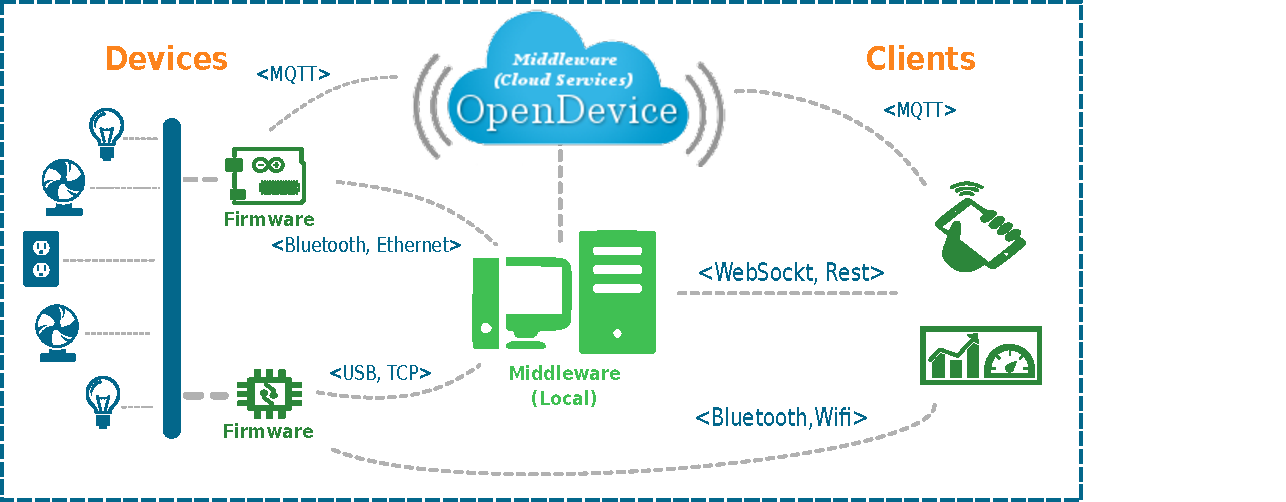
\includegraphics[width=1\linewidth]{Imagens/Cap_4/visao-geral}
\par\end{centering}
\caption{Visão Geral \label{fig:Visao-Geral}}
\end{figure}


\subsection{Componentes da Visão Geral\label{subsec:VisaoGeralComponentes}}
\begin{itemize}
\item \textbf{Middleware (Servidor)} - O middleware tem um papel fundamental
em projetos de IoT, como mencionamos na seção \ref{subsec:Fund_Middleware}.
No OpenDevice ele tem o papel de oferecer serviços para as aplicações
clientes, fazer o gerenciamento dos dispositivos, gerenciar múltiplas
conexões, fazer armazenamento e dispõe de módulos para visualização
dos dados através de dashboards dinâmicos e gráficos em tempo-real
ou históricos. Ele foi desenvolvido usando uma estrutura modular e
extensível, permitindo a inclusão de novos componentes e plug-ins
de maneira simplificada. Os desenvolvedores podem optar por utilizá-lo
como um servidor à parte, de modo embarcado ou estendendo-o. Esse
último é o modo aconselhado caso esteja desenvolvendo aplicações na
linguagem Java, pois sua arquitetura foi pensada como um framework,
de modo que os desenvolvedores de projetos de Internet das Coisas
incluam apenas as regras de negócio, sem se preocupar com os detalhes
de baixo nível. Projetos escritos em outras linguagens de programação
podem utilizar as APIs REST, MQTT, Socket e WebSocket para se comunicar
com os dispositivos através do middleware, que pode ser implantado
em um servidor local (PC / Raspberry Pi) ou na nuvem.O OpenDevice
suporta a criação de aplicações em JavaScript, que executam diretamente
na JVM (Java Virtual Machine), o que permite acesso aos módulos Java
e a criação de interfaces gráficas usando JavaFx.
\item \textbf{Firmware} - O firmware tem o papel de implementar o protocolo
do OpenDevice e fazer o gerenciamento dos dispositivos físicos (atuadores
e sensores) ligados a ele, criando uma abstração de alto nível, e
facilitando a integração com a camada de software. Nele, os dispositivos
(sensores e atuadores) são configurados e mapeados para um pino específico,
de modo que apenas as informações do dispositivo (ID, Nome, Tipo)
são expostas para as APIs externas, permitindo assim uma maior abstração
dos detalhes do hardware, ou até mesmo a substituição do hardware
por outro sem alterações na aplicação. Podemos pensar no firmware
também como um \emph{gateway,} responsável por manter a comunicação
com o middleware ou aplicação e controlar os dispositivos físicos.
É um componente de software projetado para rodar em dispositivos embarcados
com baixo poder de processamento e memória, algo em torno de 2KB de
RAM. O foco inicial do desenvolvimento foram os microcontroladores
encontrados em plataformas de prototipação como o Arduino e similares.
Com a expansão e popularidade da plataforma do Arduino inúmeros hardwares
estão dando suporte as suas APIs\cite{arduino-comp1,arduino-comp2},
ampliando a compatibilidade do firmware desenvolvido. Na seção \ref{par:Hardwares-Testados},
serão apresentados os hardwares testados. A arquitetura do firmware
é extensível, permitindo incluir novos dispositivos, novos comandos,
e suporte a novos tipos de conexões. Os detalhes do protocolo do OpenDevice
serão apresentados na seção \ref{subsec:Protocolo}. O Firmware é
um componente dispensável quando o projeto utilizar hardwares com
um maior poder de processamento e que tenham suporte a GPIO, como
no caso Raspberry ou BeagleBone. 
\item \textbf{Devices} - Representam os dispositivos físicos que podem ser
atuadores (representado pela classe \textbf{Device}) ou sensores (representados
pela classe \textbf{Sensor}). Estão organizados nos seguintes tipos:
(1) ANALOG, (2) DIGITAL, (3) CHARACTER, que estão ligados ao modo
de operação e tipo de dado suportado. Dentro do protocolo os dispositivos
são identificados através de um código, denominado DeviceID. Os dispositivos
do tipo ANALOG, podem receber uma faixa de valores numéricos, já os
dispositivos do tipo DIGITAL trabalham com dois estados: 0 (desligado)
e 1 (ligado), os dispositivos do tipo CHARACTER, estão aptos a receber
uma String. O OpenDevice trabalha com um modelo orientado a objetos,
permitindo que uma chamada dos métodos do \emph{Device} na aplicação
cliente, como por exemplo \emph{Device1.on()}, acenda uma lâmpada
real ou o realize fechamento de uma garra robótica. Eles podem ser
independentes ou estarem conectados a um microcontrolador, executando
o firmware, que faz o papel de Gateway. Os desenvolvedores podem estender
essa abstração e adicionar novos comportamentos para os dispositivos
e sensores.
\item \textbf{Clientes} - Representam as aplicações clientes, que podem
ser aplicações Desktop, web ou \emph{mobile} e podem ser desenvolvidas
em qualquer linguagem. As aplicações clientes, podem se comunicar
com o middleware, através das interfaces ofertadas (REST, MQTT, Socket,
WebSocket e etc.) ou diretamente com os dispositivos físicos. Foram
desenvolvidos módulos de bibliotecas clientes que permitem a integração
com o middleware em linguagens Java e JavaScript e experimentos de
integração usando a linguagem python. Mais detalhes sobre estas implementações
serão vistas na seção \ref{subsec:ConexoesCliente}. 
\end{itemize}

\subsection{Modelos de comunicação\label{subsec:ModelosComunicacao}}

A arquitetura planejada permite desenvolver projetos em vários Layouts
e modelos de comunicação, permitindo atender desde aplicações locais,
que se comunicam diretamente com os dispositivos, até aplicações distribuídas,
com comunicação através da internet.
\begin{itemize}
\item \textbf{Comunicação direta} - É um modelo que permite a comunicação
direta entre a aplicação final e os dispositivo físicos. Tem a característica
de ser mais simples, pois neste modelo, não se faz necessária a presença
do middleware (servidor). A aplicação neste cenário pode ser representada
por: (1) um dispositivo mobile, (2) uma aplicação desktop ou (3) uma
aplicação web. Representando o dispositivo físico, podemos ter um
hardware que disponibilize um mecanismo de comunicação embarcado,
por exemplo o ESP2866, que possui Wi-Fi, ou por exemplo um Arduino
com um módulo Bluetooth acoplado. Estes dois componentes podem se
comunicar usando diversas tecnologias, como: USB, Bluetooth, Ethernet,
Wi-Fi. Mais detalhes sobre os meios de comunicação e como eles são
implementados, serão vistos nas seções \ref{subsec:Arquitetura-do-Firmware}
e \ref{subsec:FirmwareGerenciamentoConn}.
\item \textbf{Comunicação local (Middleware)} - No modelo de comunicação
local, entre em cena um novo componente do OpenDevice, o middleware.
O middleware quando implantado dentro de um projeto pode ser visualizado
como o servidor, e pode ser configurado tanto em um computador convencional,
como em um mini-pc (ex.: Raspberry Pi). A vantagem da inclusão deste
elemento é que ele permite que diversas aplicações se comuniquem com
o mesmo dispositivo. Por exemplo, caso uma aplicação mobile esteja
conectada via Bluetooth com um dispositivo, outra aplicação será impedida
de se comunicar com esse dispositivo, usando middleware, essa limitação
é contornada, já que o middleware recebe os comandos das aplicações
cliente e faz o redirecionamento para o dispositivo desejado. Outra
vantagem é que o middleware pode gerenciar várias conexões com os
dispositivos, utilizando vários meios de comunicação, liberando essa
carga de gerenciamento das aplicações. Neste modelo de comunicação,
os dispositivos podem operar no modo servidor, aguardando a conexão
por parte do middleware, ou no modo cliente.
\item \textbf{Comunicação pela Internet} - Neste modelo as aplicações podem
se comunicar com os dispositivos através da internet. Para isso, os
dispositivos devem possuir um hardware que suporte uma conexão usando
o protocolo TCP/IP, necessitando apenas de um roteador convencional
para interligação com a internet ou um modem GSM/GPRS. Neste cenário
os dispositivos atuam no modo cliente e o middleware está implantado
em um servidor na nuvem.
\item \textbf{Comunicação pela Internet, usando um middleware local} - Neste
modelo um middleware local é aplicado novamente, permitindo que as
aplicações continuem funcionando caso a internet não esteja disponível
ou quando é necessário integrar dispositivos que não possuem suporte
o protocolo TCP/IP. Neste modelo, a mesma versão do middleware está
rodando em um servidor local e em um servidor na nuvem, diferenciando
apenas os módulos e infraestrutura utilizada, já que em um servidor
local a memória e recursos são limitados e num servidor de nuvem é
necessário uma performance e alta escalabilidade.
\end{itemize}

\subsection{Requisitos\label{subsec:Requisitos}}

A arquitetura foi projetada para ser adaptável às capacidades e necessidades
de casos de uso específicos. Esses podem ser categorizados como:
\begin{itemize}
\item \textbf{Requisitos de Comunicação} - O sistema deve ser apoiado em
eventos e/ou comunicação autônoma. Os dispositivos devem ser configurados
e controlados remotamente. O sistema deve suportar comunicação em
tempo-real. O sistema deverá fornecer comunicação segura e confiável.
O sistema deve prover recursos para extensão dos protocolos de comunicação.
\item \textbf{Gerenciamento de dispositivos} - A API deve prover uma interface
para o controle dos dispositivos. Isso inclui a configuração do dispositivo
bem como ativação, desativação e atualização remota.
\item \textbf{Serviços de Descoberta }- O sistema deve oferecer mecanismos
para descoberta e vinculação de novos dispositivos.
\item \textbf{Capacidades do dispositivo} - A API deve prover informações
sobre as capacidades dos dispositivos.
\item \textbf{Requisitos de comunicação cliente/servidor} - A API deve prover
suporte para operar os dispositivos tanto no modo cliente como no
modo servidor.
\item \textbf{Requisitos de monitoramento de status} - Status como nível
de bateria, temperatura, estado de operação dentro da infraestrutura
devem estar acessíveis.
\item \textbf{Serviço de Armazenamento} - A API deve oferecer recursos para
armazenamento das informações sobre os dispositivos, bem como mecanismo
para obter o histórico dos dados do dispositivo.
\item \textbf{Serviço de Visualização} - A API deve oferecer serviço para
análise dos dados, recursos para consultas históricas, funções para
agrupamento e agregação dos dados, bem como componentes visualização
através de gráficos.
\item \textbf{Orientado a Eventos} - O sistema deve oferecer um sistema
para tratamento de eventos, notificando as partes interessadas quando
alguma mudança de estado ocorrer nos dispositivos.
\item \textbf{Interoperável entre várias redes (PAN, LAN e WAN)} - Precisa
trabalhar através de uma variedade de redes e protocolos, tanto com
redes IP e não-IP, incluindo dispositivos de baixa potência (low-power)
em redes como Z-Wave, Zigbee e Bluetooth. 
\item \textbf{Extensível} - Deve fornecer recursos que permitam a inclusão
de novos componente e funcionalidades através de extensões ou plug-ins.
\item \textbf{Independência de Plataforma} - A API de serviços deve ser
multi-plataforma, executando nos principais sistema operacionais encontrados
no mercado.
\end{itemize}

\subsection{Extensibilidade\label{subsec:VisaoGeral-Extensibilidade}}

Toda a arquitetura do OpenDevice foi pensada visando uma fácil extensibilidade,
permitindo inclusão de novos protocolos, novos módulos de comunicação
e integração com outras ferramentas. Devido à grande diversidade de
áreas, requisitos e domínios variados que projetos de Internet das
Coisas podem ser empregadas, e por ser uma área relativamente nova,
é uma tarefa complexa desenvolver uma plataforma/Framework que atenda
a todos os requisitos. Esse trabalho oferece contribuições com uma
base sólida para criação de outros projetos especializados para outros
domínios como automação residencial, saúde, cidades inteligentes e
etc, porém sua estrutura generalista pode ser empregada para criar
vários projetos sem necessidade de modificações, no capítulo \ref{sec:Avaliacao-Experimental}
será realizada uma avaliação experimental, usando como base o domínio
da automação residencial para validar a arquitetura, com base na sua
aplicação generalista e nas suas capacidades de extensibilidade.

No contexto de extensibilidade, foram analisadas algumas estratégias
de implementação de suporte a plug-ins e módulos dinâmicos, uma das
soluções mais promissoras nesse campo é o OSGI (Open Services Gateway
Initiative)\cite{osgi}, porém foi descartado por considerarmos que
é uma ferramenta que adiciona uma complexidade extra no desenvolvimento
das extensões e necessita de um gerenciamento complexo que é feito
pelo contêiner de OSGI, consequentemente consumindo mais recursos.
A solução adotada é baseada em uma ferramenta disponível pela própria
linguagem Java, o SPI (Service Provider Interfaces), que tem como
objetivo, de oferecer recursos de extensão de forma simples e leve,
baseando-se apenas em interfaces que são definidas pelo próprio OpenDevice
e um arquivo de configuração simples. Uma pequena desvantagem encontrada
no mecanismo do SPI é que ele não permite o carregamento dinâmico
de plug-ins em tempo de execução, apenas no carregamento da aplicação.


\section{Arquitetura detalhada\label{subsec:Arquitetura-Detalhada}}

Nesta seção, veremos os detalhes da arquitetura empregada na construção
do projeto OpenDevice, analisando os módulos individualmente, os blocos
funcionais e suas responsabilidades.

Uma das considerações importantes no desenvolvimento desse projeto
é que o core da arquitetura e os módulos servidores principais~(MQTT,
Rest e WebSocket) pudessem ser executados em hardwares de baixo poder
de processamento, algo em torno de 512MB de RAM e 500Mhz de CPU. Com
base nessa restrição, foram desenvolvidos módulos de servidores que
executam em modo embarcado(\emph{embedded}), já que as soluções disponíveis
de servidores Java como: Tomcat , Jetty, JBoss ou GlassFish, iriam
consumir muitos recursos da máquina. O mesmo critério foi aplicado
na seleção do banco de dados, que é um componente opcional. Soluções
embarcadas foram adotadas em relação à soluções instaladas separadamente
(ex.: MySQL), facilitando o desenvolvimento e distribuição da aplicação.

A camada do middleware, das aplicações clientes e firmware são baseadas
no modelo de desenvolvimento orientado eventos (\emph{Event-Driven}),
realizada através do envio e recebimento de comandos, usando comunicações
em tempo-real. O modelo baseado em eventos facilita o desenvolvimento
de aplicações de IoT, principalmente quando é necessária a interação
com sensores, permitindo que os desenvolvedores registrem que tipo
de evento ou os dispositivos que desejam monitorar, e quando o evento
ocorrer, como por exemplo um sensor mudar seu valor, os interessados
no evento serão notificados. Esse modelo também permite uma fácil
extensão da ferramenta, pois tira a responsabilidade das extensões
de conhecer fluxo de conexão e aspectos internos do funcionamento,
podendo agregar funções mais elaboradas para lidar com os eventos,
como por exemplo, um algoritmo de inteligência artificial (IA) que
faça predição.

Na Figura \ref{fig:Arquitetura} pode-se observar a arquitetura e,
cada camada, assim como, cada elemento será explicado a seguir. 

\begin{figure}
\begin{centering}
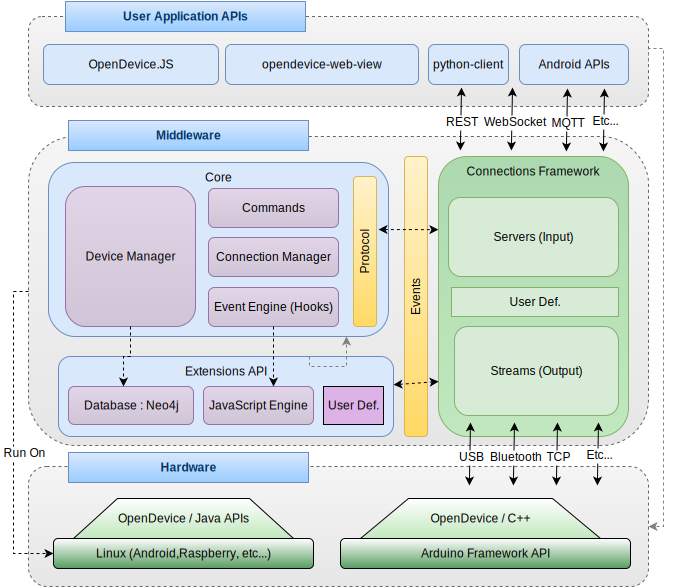
\includegraphics[width=1\linewidth]{Imagens/Cap_4/arquitetura}
\par\end{centering}
\caption{Arquitetura detalhada\label{fig:Arquitetura}}
\end{figure}


\subsection{Camadas da Arquitetura}
\begin{itemize}
\item \textbf{Camada de Aplicação (User Application APIs)} - Constituem
os módulos e bibliotecas disponibilizados para utilização pelas aplicações
clientes, permitindo a integração com o OpenDevice. A maioria dos
módulos são projetados para que as aplicações se comuniquem com os
dispositivos físicos (hardware) através do middleware, porém estão
disponíveis módulos que permitem a comunicação direta entre a aplicação
cliente e o hardware. Foram desenvolvidos módulos clientes para Web,
Desktop e Android, os detalhes da implementação e tecnologias suportadas
serão abordados na seção \ref{subsec:ConexoesCliente}.
\item \textbf{Middleware} - O middleware é uma camada altamente modular
e customizável, que oferece uma série de serviços para as aplicações,
como mencionamos na seção \ref{subsec:VisaoGeralComponentes} (Componentes
da Visão Geral). Ele é a peça central que permite a comunicação das
aplicações com os hardwares utilizando uma linguagem de alto-nível.
O middleware foi desenvolvido para uma fácil extensão, devido a essa
característica, ele se torna um framework para criação de projetos
de Internet das Coisas. Conta com um poderoso framework de conexões,
responsável pelas definições do protocolo, comunicação com os dispositivos
físicos e integração com as aplicações. Mais detalhes e sub-componentes
serão abordados a seguir.
\item \textbf{Hardware} - Os hardwares podem ser classificados em microcontroladores
e Mini PCs. Para os microcontroladores são disponibilizadas bibliotecas,
que chamamos nesse trabalho de firmware, que permitem uma fácil integração
com o middleware (servidor) e facilitam a criação de objetos inteligentes.
Elas dão suporte a utilização de várias tecnologias de comunicação,
como: Usb, Bluetooth, Ethernet e Wi-Fi. Essas bibliotecas são baseadas
no framework do Arduino, o que as tornam compatíveis com uma séries
de Hardwares e plataformas de prototipação, inclusive que não fazem
parte do projeto do Arduino\cite{arduino-comp1,arduino-comp2,arduino-comp3}.
Quando se trata de Mini PCs, que envolvem hardwares de maior poder
de processamento e memória, como por exemplo, Raspberry~Pi e BeagleBone,
é possível executar o middleware diretamente neles, desde que se tenha
disponível uma implementação da JVM para esses dispositivos. Nos Mini
PCs, o acesso aos pinos de GPIO ainda é um problema, pois cada hardware
possui suas especificações. O projeto Device I/O \cite{device-io:wiki},
mantido pela comunidade do OpenJDK, tem a proposta de criar uma implementação
para o acesso aos periféricos desses dispositivos, porém ainda está
em fase de desenvolvimento. Para hardwares não suportados pelo projeto,
existem três alternativas: (1) criar adaptadores/Wrapper para bibliotecas
já existentes, (2) implementar chamadas JNI ou (3) usar o drivers
baseados em \emph{Sysfs} que alguns Kernels disponibilizam para acessar
a GPIO como fossem simples arquivos\cite{key-sysfs}.
\end{itemize}

\subsection{Módulos}

Nesta seção, abordaremos os módulos que compõe a arquitetura. Na Figura
\ref{fig:Modulos} pode-se observar os módulos, assim como, cada elemento
será explicado a seguir. 

\begin{figure}
\begin{centering}
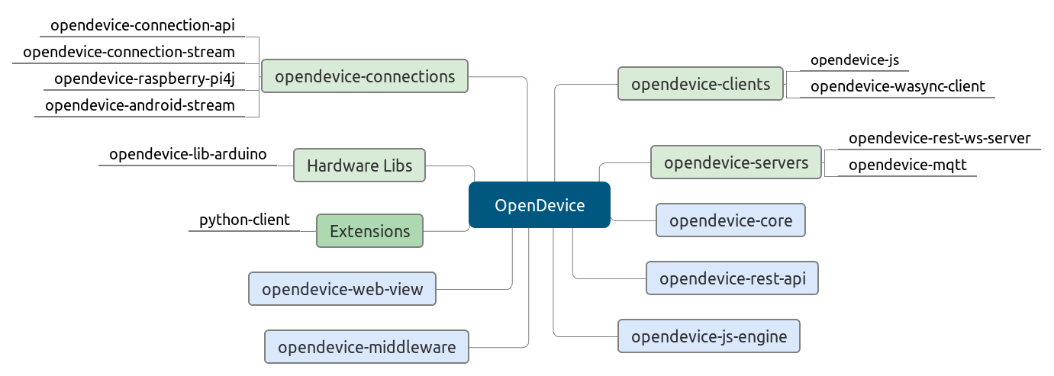
\includegraphics[width=1\textwidth]{/media/ricardo/Dados/Dropbox/Mestrado/Dissertacao/Imagens/Cap_4/OpenDevice_Modulos}
\par\end{centering}
\caption{Módulos\label{fig:Modulos}}
\end{figure}

\begin{enumerate}
\item Módulos Gerais

\begin{enumerate}
\item \noun{core}: Módulo base da arquitetura, com o sistema de gerenciamento
de dispositivos, sensores, conexões, eventos, armazenamento, API de
comandos e implementação do protocolo. Esse módulo pode ser usado
no desenvolvimento de aplicações Desktop, Web ou Mobile;
\item \noun{rest-api}: Definições das interfaces REST para controle dos
dispositivos e sensores;
\item \noun{js-engine: }Implementação do suporte a execução de JavaScript
no lado do servidor;
\item \noun{web-view}: Interface HTML/5 + AngularJS + OpenDeviceJS;
\item \noun{middleware: }Aplicação de gestão, controle e monitoramento,
que usa a maior parte dos módulos do OpenDevice, usando o banco de
dados Neo4J + Hibernate OGM (JPA).
\end{enumerate}
\item Módulos do framework de conexões

\begin{enumerate}
\item \noun{connection-api}: Especificação das interfaces de conexão cliente/servidor;
\item \noun{connection-stream}: Implementações de conexões USB, Bluetooth,
TCP (PC/RaspPI);
\item \noun{android-stream}: Implementação de conexões USB, Bluetooth para
Android\footnote{\begin{enumerate}
\item Demais conexões (Rest, WebSocket, MQTT) podem ser utilizada no Android
através dos outros módulos.
\end{enumerate}
};
\item \noun{raspberry-pi4j}: Comunicação com a GPIO do Raspberry usando
PI4J.
\end{enumerate}
\item Módulos Cliente

\begin{enumerate}
\item \noun{opendevice-js}: Biblioteca JavaScript com suporte a WebSocket
e REST;
\item \noun{opendevice-wasync-client}: Biblioteca WebSocket para Android
e PC;
\item \noun{python-client}: Biblioteca em Python com suporte a TCP.
\end{enumerate}
\item Módulos Servidores

\begin{enumerate}
\item \noun{rest-ws-server}: Servidor REST e WebSocket;
\item \noun{opendevice-mqtt}: Servidor MQTT;
\end{enumerate}
\item Bibliotecas para hardware

\begin{enumerate}
\item opendevice-lib-arduino: Bibliotecas em C++ baseadas na API do Arduino,
que implementa o protocolo do OpenDevice e são usadas para criação
do firmware. Provê suporte ao gerenciamento de dispositivos e conexões:
USB, Bluetooth, Wi-Fi, Ethernet. Veja a lista de placas testadas na
seção~\ref{par:Hardwares-Testados}.
\end{enumerate}
\end{enumerate}

\section{Gerenciamento de Dispositivos\label{sec:GerenciamentoDispositivos}}

Um dos principais requisitos de uma arquitetura de Internet das Coisas
é realizar a abstração dos dispositivos, permitindo lidar com a sua
grande heterogeneidade. No OpenDevice as abstrações base são implementadas
através das classes Device e Sensor. Algumas implementações de clientes
sofrem algumas variações nessa abstração, como por exemplo no cliente
JavaScript \noun{opendevice-js,} onde existe apenas a classe \emph{Device}
e a identificação, se é um sensor ou atuador, é feita através de um
atributo, já que nessa linguagem não temos suporte a orientação a
objetos. 

O OpenDevice permite a conexão com vários hardwares ao mesmo tempo,
cada hardware (ex.: Arduino) pode gerenciar vários sensores e atuadores,
cada sensor e atuador é interpretado como um ``\emph{Device}'' e
recebe um ID (DeviceID) único na plataforma, que pode ser codificado
manualmente ou dinamicamente. Quando o módulo cliente ou o middleware
estabelece uma conexão com o hardware (ex.: Arduino), ele solicita
as definições dos dispositivos que foram configurados. A biblioteca
(firmware) instalada no hardware, cuida de todo o processo de negociação.
A configuração de dispositivos no hardware pode ser feita de forma
estática, através de uma pre-configuração, ou dinâmica, através de
comandos. No hardware, os dispositivos são mapeados de forma a vincular
o pino do microcontrolador com um ID (DeviceID), de modo que as aplicações
externas conheçam o apenas ID, criando uma abstração do hardware final,
permitindo mudanças sem afetar a aplicação. Os hardwares, atuariam
como um Gateway, podendo ser identificados através de um nome ou ID,
e seriam responsáveis por controlar sensores e atuadores, e integra-los
às aplicações. 

A listagem \ref{alg:devices1} apresenta um exemplo (em Java) da configuração
dos dispositivos e conexão. Ao instanciar uma classe Device dentro
de uma classe que estende \emph{LocalDeviceManager, }eles passam a
ser gerenciados pelo OpenDevice, e qualquer alteração dos valores
dos dispositivos (ex.: \emph{led.on()} e \emph{led.off()}), resulta
em um envio de um comando para o hardware, que verifica o ID do dispositivo
e faz o mapeamento para o pino correspondente. No lado do hardware/firmware
(listagem \ref{alg:devices2}), a configuração dos dispositivos foi
realizada de forma estática, onde foram adicionados dois dispositivos:
(1) um atuador digital (led), conectado no pino 5 do Arduino e (2)
um sensor digital (switch), conectado no pino 3. A associação do ID
para cada dispositivo foi realizada de forma automática e sequencial,
porém é possível especificar um ID manualmente. 

Ao pressionar o sensor físico (ID=2), o firmware reconhece a alteração
no seu estado e envia uma notificação para a aplicação (ou middleware),
que chama o evento ``onChange'' do dispositivo especificado e notifica
outros componentes (incluindo extensões) que foram registrados para
esse evento. No evento disparado, no exemplo na listagem \ref{alg:devices1},
ele verifica o status atual do botão (linha 11), se estiver ligado/pressionado,
ele chama o método \emph{``on()''} do led. O OpenDevice detecta
essa alteração e envia o comando para o hardware (firmware) e este
faz o acionamento do pino correspondente ao dispositivo. Mais detalhes
sobre os fluxos de execução de comandos são apresentados na seção
\ref{subsec:FluxoMensagens}.

O exemplo apresentado demonstra a integração entre uma aplicação e
um hardware baseado em um microcontrolador, que tem um recursos extremamente
limitados. Em hardwares com maior poder de processamento, denominados
Mini-PCs (ex.: Raspberry), é possível executar a aplicação e fazer
o controle dos dispositivos diretamente, pois ele permite acesso aos
periféricos (pinos GPIO). A listagem \ref{alg:devices3}, apresenta
um exemplo resumido de como realizar o mapeamento dos dispositivos
para os pinos correspondentes do RaspberryPi.

\begin{algorithm}[H]
\inputencoding{latin9}\begin{lstlisting}[numbers=left]
// alguns trechos de c�digo foram omitidos
public class BlinkButtonDemo extends LocalDeviceManager{

    public BlinkButtonDemo() {

        final Device led = new Device(1, Device.DIGITAL);
        final Device btn = new Sensor(2, Device.DIGITAL);

        connect(out.bluetooth("00:13:03:14:19:07"));

        btn.onChange(device -> {
            if(btn.isON()){
                led.on();
            }else{
                led.off();
            }
        });
    }
}
\end{lstlisting}
\inputencoding{utf8}
\caption{Configuração dos dispositivos - Java\label{alg:devices1}}
\end{algorithm}

\begin{algorithm}[H]
\inputencoding{latin9}\begin{lstlisting}[language={C++}]
// alguns trechos de c�digo foram omitidos
void setup(){
    ODev.name("ModuleName");
    ODev.addDevice(5, Device::DIGITAL); // ID:1 - led 
    ODev.addSensor(3, Device::DIGITAL); // ID:2 - button
    ODev.begin(Serial1, 9600);
}

void loop(){
  ODev.loop();
}
\end{lstlisting}
\inputencoding{utf8}
\caption{Configuração dos dispositivos no Arduino - Firmware/C\label{alg:devices2}}
\end{algorithm}

\begin{algorithm}[H]
\inputencoding{latin9}\begin{lstlisting}[language={C++}]
// alguns trechos de c�digo foram omitidos
Device led = new Device(1, DeviceType.DIGITAL).gpio(1);
// ...
connect(new RaspberryGPIO());
\end{lstlisting}
\inputencoding{utf8}
\caption{Configuração dos dispositivos no Raspberry - Java \label{alg:devices3}}
\end{algorithm}


\section{Modelo Orientado a Eventos\label{sec:ModeloEventos}}

O design da arquitetura segue um modelo orientado a eventos, ou \emph{Event-Driven},
que permite desacoplar os componentes da arquitetura e aplicações.
Este desacoplamento pode ser de tempo, espaço ou sincronização\cite{key-eventd}. 

O mecanismo de eventos é importante na construção do framework, pois
ele é considerado mais eficiente e escalável do que o modelo baseado
em \emph{Polling}, que é um mecanismo síncrono de requisição e resposta,
que pode introduzir uma latência na comunicação e no tempo de resposta\cite{key-poll2}.
Esse mecanismo também permite a isolação das aplicações, de saber
qual a frequência com que os dispositivos geram os dados, passando
apenas a utilizar um mecanismo de ``observar'' os dispositivos,
e reagir aos eventos quando eles acontecem.

Os eventos gerados pelas aplicações clientes, são direcionados para
o middleware ou diretamente para os dispositivos, de forma automática
e transparente. Os principais eventos gerados pela arquitetura são:
mudança do estado do dispositivo, associação de novos dispositivos,
mudança no estado das conexões, porém exitem outros e novos podem
ser criados. È possível monitorar eventos gerados por dispositivos
individuais, registrado ouvintes (listeners) para as instâncias especificas,
ou para todos os dispositivos, registando ouvintes (listeners) no
gerenciador de dispositivos (\emph{DeviceManager}).

Um exemplo foi apresentado na seção \ref{sec:GerenciamentoDispositivos},
listagem \ref{alg:devices1}, onde é adicionado um ``ouvinte'' no
dispositivo e quando o valor dele mudar, o ``ouvinte'' é executado.
No exemplo citado, o ``ouvinte'' ao ser executado, faz a chamada
do método ``led.on()'', gerando um evento (comando) que é despachado
para os componentes interessados. Um dos interessados é o \emph{CommandDelivery},
que cuida do envio e monitoramento da entrega do comando, através
das conexões de saída. Outro interessado é o serviço de armazenamento
que, se habilitado, registra o histórico de alterações dos valores
dos dispositivos.

Algumas bibliotecas disponibilizadas para construção de aplicações
clientes se baseiam no sistema Publish/Subscribe, que permite um
baixo acoplamento e uma alta escalabilidade. Um dos exemplos é a
biblioteca JavaScript para desenvolvimento de aplicações WEB, \noun{opendevice-js},
que utiliza o procolo de comunicação WebSocket e consegue interagir
(envio e recebimento) com os dispositivos praticamente em tempo-real.


\section{API de Comandos\label{sec:APIComandos}}

As informações trocadas entre hardware, middleware e aplicações clientes
são baseadas em mensagens, que são chamadas de comandos e são representadas
pela classe base \emph{Command}. Esses comandos são convertidos no
protocolo do OpenDevice (mais detalhes serão vistos na seção \ref{subsec:Protocolo}),
através dos serializadores. O framework permite a comunicação com
os hardwares e controle dos dispositivos, utilizando apenas os comandos,
sem utilizar as abstrações obtidas com os dispositivos (classe \emph{Device}
e \emph{Sensor}). A listagem \ref{alg:command} mostra um exemplo
da equivalência da operação usando a classe \emph{Device} e usando
os comandos. A classe DeviceCommand, permite o envio de comandos do
tipo DIGITAL e ANALÓGICO. O recebimento de informações geradas pelo
hardware ou de outro componente (ex.:aplicação cliente), é realizada
através de comandos. Para realizar o monitoramento e recebimento desses
comandos é necessário adicionar os ouvintes (listeners) nas conexões,
um exemplo simplificado é apresentado na listagem \ref{alg:command-1}.
Ao enviar um comando para o hardware, ele irá responder com uma mensagem
de status, que é representada pela classe \emph{ResponseCommand},
permitindo identificar se os comandos foram recebidos corretamente
ou não. O envio das mensagens é gerenciado pelo \emph{CommandDelivery},
que permite direcionar a mensagem para a conexão certa e monitorar
a entrega. Caso ela não seja feita, devido a um delay ou falha de
comunicação, ele notifica a aplicação com um erro de \emph{timeout}
detalhes desse fluxo serão apresentados na seção \ref{subsec:FluxoMensagens}.
A figura \ref{fig:DiagCommands} mostra um diagrama de classe simplificado
da API de comandos. Essa API promove mais uma camada de abstração,
permitindo que, caso as implementações atuais dos dispositivos (Device
e Sensor) não sejam suficientes, elas possam ser substituídas.

\begin{algorithm}[H]
\inputencoding{latin9}\begin{lstlisting}[language={C++}]
// Usando a API de comandos
DeviceConnection conn = Connections.out.usb();
conn.send(DeviceCommand.ON(1)); // '1' is DeviceID

// Usando a abstra��o
Device led = new Device(1, Device.DIGITAL);
led.on();
\end{lstlisting}
\inputencoding{utf8}
\caption{Comparação da API de comandos e Devices \label{alg:command}}
\end{algorithm}

\begin{algorithm}[H]
\inputencoding{latin9}\begin{lstlisting}[language={C++}]
DeviceConnection conn = Connections.out.usb();
conn.addListener(new ConnectionListener() {
    public void onMessageReceived(Message message, DeviceConnection connection) {
        String type = message.getClass().getSimpleName();
        System.out.println("onMessageReceived("+type+"): "+ message);
    }
});
\end{lstlisting}
\inputencoding{utf8}
\caption{Monitorando recebimento de comandos \label{alg:command-1}}
\end{algorithm}

\begin{figure}
\begin{centering}
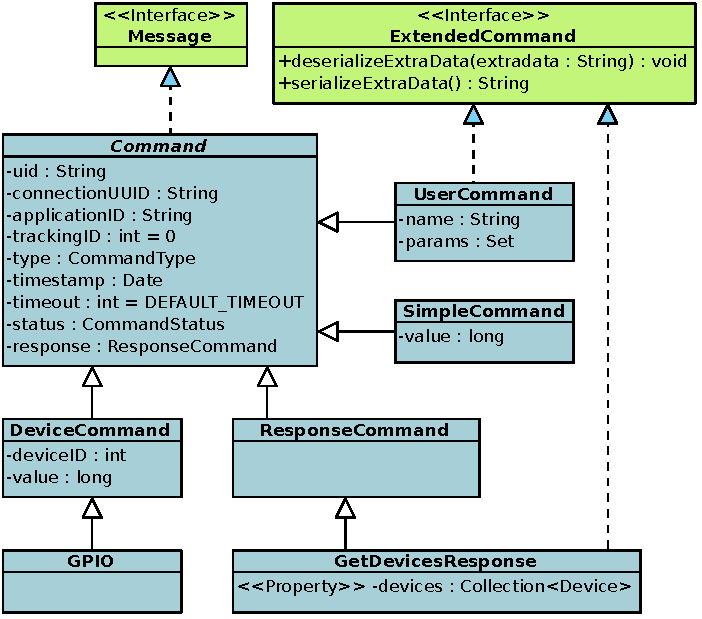
\includegraphics[width=0.7\linewidth]{Imagens/Cap_4/commands-api}
\par\end{centering}
\caption{Diagrama de classe simplificado dos Comandos\label{fig:DiagCommands}}
\end{figure}


\section{Mecanismo de extensão\label{sec:MecanismoExtensao}}

Como mencionado na seção \ref{subsec:VisaoGeral-Extensibilidade},
o mecanismo de extensão da arquitetura é baseado no SPI (Service Provider
Interface), um recurso simples e leve, disponível no Java 6 e posteriores.
Embora a arquitetura tenha sido projetada como um framework, para
ser usado como base para criação de projetos mais especializados,
existe uma implementação padrão, denominada \emph{middleware}, que
permite customizações através de extensões/plug-ins. Os mecanismos
de extensão padrão estão voltados para: (1) conexões, permitindo adicionar
novas conexões ou substituir por implementações mais eficientes, (2)
tratadores de eventos, que permitem plugar estratégias de tratamento
de eventos, e (3) sistema de armazenamento. As extensões são implementadas
através da interface \emph{OpenDeviceExtension}, que são inicializadas
durante o carregamento da aplicação. Para que as extensões sejam carregadas
corretamente é necessário que no módulo (.jar), seja incluído o arquivo
de configuração na pasta: \emph{resources/META-INF/services,} com
o nome:\emph{ br.com.criativasoft.opendevice.engine.js.ExtensionPoint},
seguindo as especificações do SPI. As conexões seguem um mecanismo
similar, porém possuem seus pontos de extensão individualizados para
cada tipo de conexão, como foi visto na figura \ref{fig:DiagConections}.


\subsection{Framework de Conexões\label{subsec:Framework-de-Conexoes}}

O framework de conexões foi projetado para ser usado de forma independente
do restante da arquitetura. A figura \ref{fig:DiagConections} mostra
a hierarquia base das conexões suportadas pela arquitetura. Essas
interfaces são os pontos de extensão, permitindo que implementações
possam ser utilizadas de acordo com a plataforma ou mesmo trocadas
por uma implementação mais eficiente. A figura \ref{fig:DiagConections2}
mostra um exemplo de implementação da conexão Bluetooth. A implementação
para aplicações Desktop é fornecida pelo módulo \noun{connection-stream},
já a implementação para aplicações Android são fornecidas pelo módulo
\noun{android-stream}, dessa maneira é possível que uma aplicação
possa ser portada sem modificações no seu código base para outras
plataformas. No OpenDevice a implementação correta é escolhida pela
fábrica de conexões, usando \emph{Connections.out.bluetooth(``...'').}
Esta fábrica está disponível no módulo core, e possui método para
criação das principais tecnologias de comunicação suportadas, tanto
clientes, como servidores. Os principais componentes desse framework
e suas descrições são listadas a seguir.

\begin{figure}
\begin{centering}
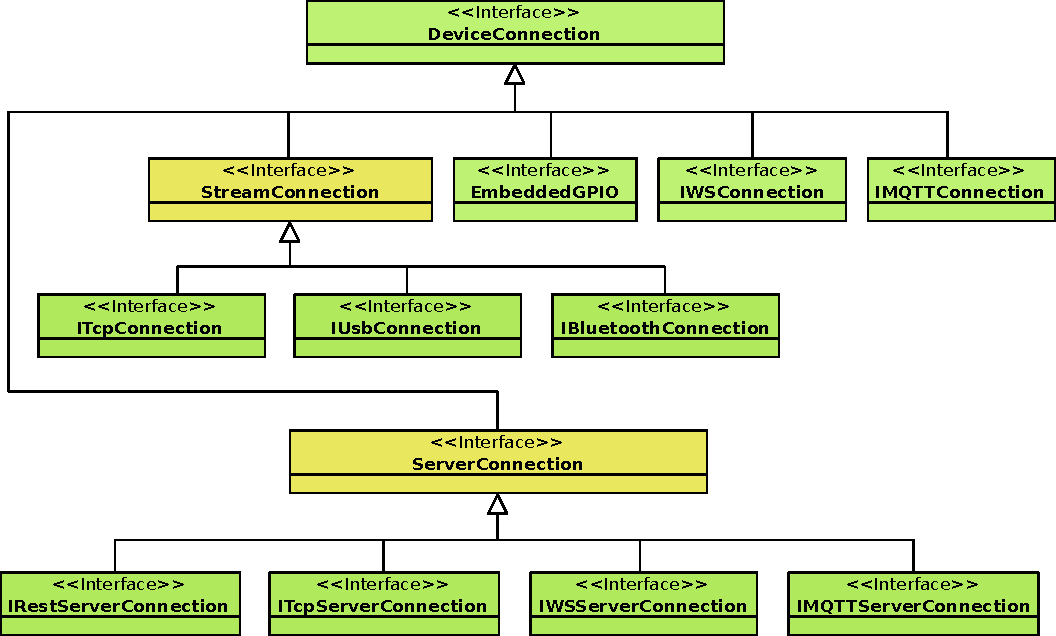
\includegraphics[width=1\linewidth]{Imagens/Cap_4/connections}
\par\end{centering}
\caption{Diagrama de classe das conexões\label{fig:DiagConections}}
\end{figure}

\begin{figure}
\begin{centering}
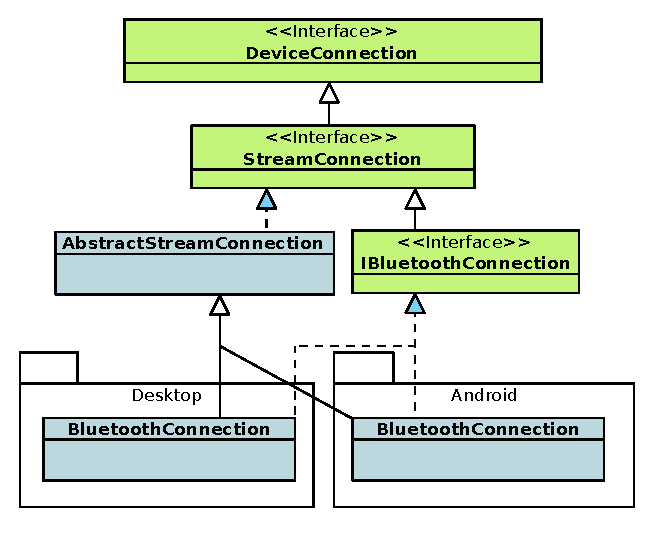
\includegraphics[width=0.7\linewidth]{Imagens/Cap_4/connections-bluetooth}
\par\end{centering}
\caption{Exemplo de implementação da conexão bluetooth\label{fig:DiagConections2}}
\end{figure}

\begin{itemize}
\item DeviceConnection - Interface base para todos as conexões do sistema,
define o modo de operação geral das conexões e em conjunto com o \emph{MessageSerializer}
define o modelo de protocolo a ser utilizado. Possui uma implementação
base, através da classe \emph{AbstractConnection}, que facilita a
criação de implementações finais. 
\item MessageSerializer - Como mencionado anteriormente, é o componente
responsável pela serialização e desserialização das mensagens enviadas
e recebidas pelas conexões. São as implementações que definem o tamanho
e formato das mensagens. A implementação padrão, localizada no módulo
core, é feita pela classe \emph{CommandStreamSerializer}. 
\item ConnectionListener - Interface que permite monitorar de forma plugável
os eventos ocorridos na conexão, como conexão, desconexão e recebimento
de mensagens, permitindo às aplicações reagirem à esses eventos. Vários
ouvintes de eventos (Listeners) podem ser adicionados àconexão.
\item Message - Interface que encapsula os dados enviados e recebidos, exemplos
de implementações são \emph{ByteMessage}, \emph{Request}, etc. A implementação
base usada no OpenDevice é realizada pela classe \emph{Command}, localizada
no módulo core.
\end{itemize}
No OpenDevice, esse framework é utilizado em duas camadas: (1) conexões
de entrada (Input), que são os servidores e têm por objetivo disponibilizar
os serviços para as aplicações clientes, como por exemplo o servidor
REST, e (2) conexões de saída (Output), denominados na maioria das
vezes como streams, que são as conexões com os módulos físicos (hardware)
e que implementam o protocolo de baixo nível, realizando a serialização
e desserialização dos comandos enviadas pelas aplicações. 

\section{Módulos Servidores \label{subsec:ConexoesServidores}}

Os módulos servidores, são responsáveis por fazer a interface com
as aplicações clientes. Eles permitem a inclusão de novos mecanismos
de conexão ou novos protocolos. Um exemplo de utilização de novo protocolo
é encontrado no servidor REST, que expande o protocolo do OpenDevice
(\ref{subsec:Protocolo}), permitindo criar interfaces mais simples
e de mais alto nível para as aplicações cliente se comunicarem com
os dispositivos.

O servidor WebSocket permite que aplicações (Web, Desktop, Mobile)
se comuniquem em tempo real e de forma bidirecional com os dispositivos,
usando middleware. O framework é projetado seguindo dois conceitos
de conexões: (1) conexões de entrada (Input), que são os servidores,
e (2) conexões de saída (Ouput), que são as conexões com os dispositivos
físicos. O papel do middleware é realizar a tradução dos protocolos
de entrada e converte-los para os protocolos de saída, específicos
para cada dispositivo, confirme a figura \ref{fig:middleware_connections}.
O módulo de visualização (com gráficos e dashboards), apresentado
na seção \ref{sec:Visualizacao}, utilizam as conexões em WebSocket
para permitir a comunicação em tempo-real com os dispositivos.

Os servidores permitem a abstração e desacoplamentos entre dispositivos
e aplicações, de modo que uma aplicação pode se comunicar com vários
dispositivos, ou permitir que varias aplicações se comuniquem com
o mesmo dispositivo, contornando alguns problemas das conexões que
suportam apenas um cliente, como no caso do Bluetooth e USB.

Os servidores foram projetados pensando na otimização de recursos
do hardware. Como o objetivo é permitir que eles possam executar em
hardwares, na categoria Mini-PCs, como o Raspberry e BeagleBone, as
implementações dos servidores utilizados no middleware, foram escolhidas
de modo que rodassem de forma embarcada e compartilhado o máximo de
recursos possíveis. Devido a arquitetura estar projetada para suportar
inicialmente os protocolos HTTP, Rest, WebSocket e MQTT, a implementações
dos mesmos seriam um desafio, devido a variedade de requisitos, estaria
fora do escopo da proposta deste trabalho. Foi então realizado um
estudo que mapeou as implementações desses protocolos individualmente,
e observou-se que as soluções mais maduras estavam baseadas em frameworks
de rede. Os principais frameworks encontrados foram: Jetty (Eclipse)\footnote{http://www.eclipse.org/jetty/},
Grizzly (GlassFish)\footnote{https://grizzly.java.net} e Netty\footnote{http://netty.io}.
O Jetty é um contêiner de aplicações Java e servidor web, que tem
uma estrutura modular e suporta protocolos como Http e WebSocket.
Apesar ser possível executar de forma embarcada, sua estrutura foi
planejada para executar aplicações Java web (.war), não como um framework
genérico e nem com plataformas embarcadas em mente. O Grizzly por
sua vez é projetado como um framework, e utilizado como base na construção
do servidor de aplicação GlassFish, suportando também HTTP, WebSocket
e sendo de fácil extensão. Por fim, o Netty, é também um framework
que tem uma estrutura simples, é utilizado para construção de projetos
como Apache Spark, Elasticsearch, Neo4j (banco de dados), Minecraft
e outros\footnote{http://netty.io/wiki/adopters.html}. O Netty é
framework utilizado como base das implementações dos servidores escolhidos
para o projeto arquitetura. 

A escalabilidade da arquitetura pode ser alcançada, substituindo os
implementações dos servidores embarcados, por implementações mais
robustas, que permitam escalonamento horizontal e balanceamento de
carga. Isto pode ser alcançado, de forma transparente para a aplicação,
utilizando os mecanismos de extensão (\ref{subsec:VisaoGeral-Extensibilidade},
\ref{sec:MecanismoExtensao}).

\begin{figure}
\begin{centering}
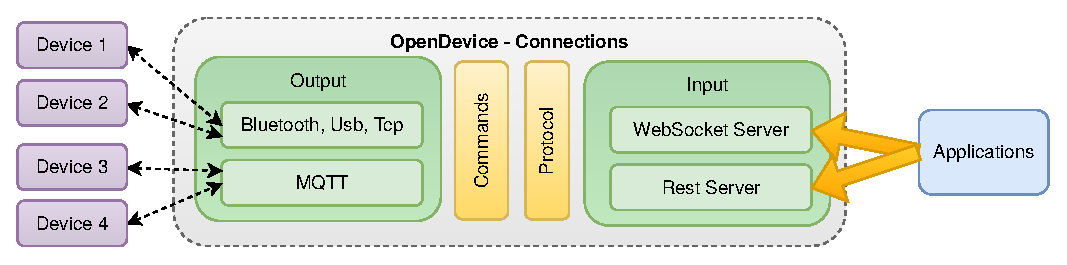
\includegraphics[width=0.8\linewidth]{Imagens/Cap_4/middleware_connections}
\par\end{centering}
\caption{Abstração dos protocolos de comunicação\label{fig:middleware_connections}}
\end{figure}


\subsection{Servidor MQTT}

A implementação de servidor MQTT escolhida, foi o ``Moquette MQTT'',
projeto mantido pela fundação Eclipse, e que utiliza como base o framework
de rede Netty.

Os servidores são em sua maioria destinados à comunicação com as aplicações
clientes (conexões de entrada). O MQTT é uma exceção, pois permite
que os dispositivos físicos também sejam conectados ao middleware.
Para permitir um gerenciamento e integração com o middleware, e permitir
a comunicação bidirecional entre aplicações e dispositivos físicos,
algumas convenções foram adotadas na nomenclaturas dos tópicos. 

Tanto as aplicações como os dispositivos físicos são ``publish''
e ``subscriber''. O middleware é o encarregado de monitorar as mensagens
e fazer o direcionamento adequado, atuando como espécie de ``subscriber''
geral. Caso uma aplicação envie uma requisição para um dispositivo,
é papel do middleware fazer o direcionamento para o tópico correto,
e monitorar a resposta e envia-la de volta (publish) para a aplicação
que fez a requisição. A camada das aplicações não conhecem a estrutura
de tópicos do borker MQTT e seu mapeamento para os dispositivos, elas
apenas possuem as abstrações dos dispositivos, orientadas a objetos,
e enviam os comandos para o middleware (ex.: device.on()). Isso mermite
que aplicações clientes MQTT consigam se comunicar com dispositivos
Bluetooth e MQTT de forma transparente.

A tabela \ref{tab:mqtt_nomenclatura}, apresenta as nomenclaturas
estabelecias para o nome dos tópicos. Quando uma aplicação realiza
uma operação na abstração do dispositivo (ex.: device.on()), um comando
é enviado para tópico ``ProjectID/middeware/in'', que é o canal
que o middleware usa para o recebimento dos comandos das aplicações.
Na implementação atual, por ser embarcada, o recebimento é feito diretamente
sem necessidade do middleware se inscrever nos tópicos. O middleware
identifica o dispositivo e determina qual conexão que o dispositivo
em questão está vinculado, que pode ser uma conexão Bluetooth ou MQTT,
nesse ultimo caso, o firmware envia (publish) o comando para seu respectivo
tópico: ``ProjectID/in/ModuleName''.

O componente denominado ``Firmware'' é um hardware (ex.: arduino)
que pode estar gerenciando um ou mais dispositivos (sensores e atuadores),
onde internamente cada um recebe uma identificação (DeviceID). Cada
conexão com um hardware recebe uma identificação chamada ``ModuleName''.

\begin{table}[h]
\begin{centering}
\begin{tabular}{|c|c|c|c|}
\hline 
Componente & Operação & Tópico & Descrição\tabularnewline
\hline 
\hline 
Firmware & Publish & ProjectID/out & Envio de Dados\tabularnewline
\hline 
Firmware & Subscribe & ProjectID/in/ModuleName & Recebimento de comandos\tabularnewline
\hline 
Middleware & Subscribe{*} & ProjectID/out & {*} Monitoramento (Listener)\tabularnewline
\hline 
Middleware & Subscribe{*} & ProjectID/middeware/in & {*} Monitoramento (Listener)\tabularnewline
\hline 
App & Publish & ProjectID/middeware/in & Envio de Comandos\tabularnewline
\hline 
App & Subscribe & ProjectID/middeware/out & Notificações Gerais\tabularnewline
\hline 
App & Subscribe & ProjectID/middeware/out/CID & Tópico de Resposta\tabularnewline
\hline 
\end{tabular}
\par\end{centering}
\caption{Nomenclatura de tópicos MQTT\label{tab:mqtt_nomenclatura}}
\end{table}


\subsection{Servidores WebSocket, Rest e Http}

O WebSocket é o protocolo originalmente utilizado para permitir a
comunicação em tempo-real com as aplicações Web, porém é possível
a sua utilização em aplicações Desktop. A implementação desse protocolo
é fornecida pelo projeto Nettosphere\footnote{https://github.com/Atmosphere/nettosphere},
também baseado no framework Netty. O grande diferencial é que ele
oferece a implementação dos três protocolos utilizando a mesma porta
(ex.: 80), e consequentemente poupando muitos recursos do hardware.
Isso é possível devido a estrutura de processamento do framework Netty,
que permite identificar e processar cada protocolo separadamente.
Teoricamente o mesmo poderia ser feito para o protocolo MQTT, mas
seria um desafio atingir o nível de maturidade da implementação embarcada
que adotamos.

O servidor HTTP, permite a configuração de pastas de recursos como
HTML, CSS e imagens, permitindo a criação de interfaces gráficas.

O servidor REST, permite a criação de serviços que atendem ao protocolo
REST. A integração com o Jesey\footnote{https://jersey.java.net},
permite a implementação da especificação Java \emph{(JAX-RS - The
Java API for RESTful Web Services}), facilitando e padronizando a
criação de novos serviços, estendendo as capacidades do \emph{middleware}.
Os serviços Rest criados, contam com suporte a injeção de dependências,
seguindo a especificação JSR-330, que se utilizam das anotações \emph{@Inject
e @Named}, para injeção dos componentes.

\section{Suporte a JavaScript\label{subsec:SuporteJavaScript}}

O suporte a JavaScript permite a criação de aplicações simples e tratadores
de eventos, que rodam nativamente, e é integrado ao OpenDevice através
do mecanismo de extensões. Também é possível criar aplicações Web,
utilizando JavaScript, com auxílio da biblioteca \noun{opendevice-js,
}que permite a abstração dos dispositivos e implementa os protocolos
REST e WebSocket.

No primeiro caso, é possível criar aplicações que executa nativamente,
ou seja, sem depender de um navegador, pois rodam diretamente na JVM,
Este suporte é fornecido através do módulo \noun{js-engine}, que usa
os recursos da própria JVM implementados no projeto Nashorn \footnote{http://openjdk.java.net/projects/nashorn/}.
Este recurso auxilia na sua utilização por desenvolvedores que não
têm experiência com linguagem Java ou mesmo desenvolvedores experientes
que precisam realizar uma prototipação mais rápida ou pela simplicidade
da implementação de tratamento de eventos com uma linguagem de script.
Devido a necessidade de recursos avançados da JVM, esse módulo (\noun{js-engine})
depende da versão Java 8, que inclui várias melhorias de performance
e integração com JavaScript. Os modos de desenvolvimento serão detalhados
a seguir.

\subsection{Criação de aplicações nativas em JavaScript}

As aplicações criadas em JavaScript, executam na JVM e têm interoperabilidade
com as classes definidas em Java. Desse modo é possível realizar chamadas
nas classes e métodos do OpenDevice. A listagem \ref{alg:ExemploJS1},
demonstra um exemplo de criação de uma aplicação simples, que ao detectar
uma mudança no botão~(BUTTON), controla o estado da lâmpada~(led).
O módulo \noun{js-engine} pode ser compilado para um executável (odevjs.exe
ou odevjs.jar), destinado a execução de aplicações em JavaScript usando
o comando: \inputencoding{latin9}\lstinline!> odevjs.exe myscript.js!\inputencoding{utf8}.

Outro exemplo de aplicação, usando interface gráfica (GUI) em JavaFX,
pode ser encontrado no Apêndice \ref{chap:ApendiceA}. Para habilitar
o JavaFX é necessário informar o parâmetro ``-fx'', exemplo: \inputencoding{latin9}\lstinline!> odevjs.exe -fx myscript.js!\inputencoding{utf8}.
Os códigos JS podem ser executados diretamente de aplicações Java,
através da classe \emph{OpenDeviceJSEngine}, exemplo: \inputencoding{latin9}\lstinline!OpenDeviceJSEngine.run("myscript.js")!\inputencoding{utf8}.

\begin{algorithm}[H]
\inputencoding{latin9}\begin{lstlisting}
var led = new Device(1, DIGITAL);
var button = new Sensor(2, DIGITAL);

button.onChange(function(){
    if(button.isON()){
        led.on();
    }else{
        led.off();
    }
});

connect(usb());
\end{lstlisting}
\inputencoding{utf8}
\caption{Exemplo de Aplicação em JavaScript\label{alg:ExemploJS1}}

\end{algorithm}


\subsection{Tratadores de Eventos (EventHook)}

Os tratadores de evento (EventHook), são pequenos trechos de código
JavaScript que estão vinculados os dispositivos (Devices e Sensors)
e são executados quando acontece alguma mudança do seu valor. Esse
mecanismo é uma extensão para o EventManager, e implementada pela
classe \emph{JavaScriptEventHandler}. A implementação padrão faz o
carregamento dos scripts através de arquivos, mas pode-se implementar
outras formas de armazenamento/carregamento. Na implementação atual
os eventos são mapeados para os dispositivos através de metadados
incluídos no próprio script. Na listagem \ref{alg:ExemploJS2}, é
implementado a mesma lógica da listagem \ref{alg:ExemploJS1}, entretanto,
eles não são interpretados através do executável (odevjs.exe), eles
são gerenciados pelo middleware e são executados quando os dispositivos
mapeados através da anotação \noun{@devices,} sofrem alguma modificação.
A variável ``device'', é injetada pelo framework e representa o
dispositivo que sofreu a alteração.

\begin{algorithm}[H]
\inputencoding{latin9}\begin{lstlisting}[language=VBScript]
/**
 * @name ButtonHookDemo
 * @devices 2
 * @description TestCase
 * @type JavaScript
 */
var led = findDevice(1);
if(device.isON()){
    led.on();
}else{
    led.off();
}
\end{lstlisting}
\inputencoding{utf8}
\caption{Exemplo do ``EventHook'' em JavaScript\label{alg:ExemploJS2}}
\end{algorithm}


\subsection{Criação de aplicações WEB em JavaScript}

A biblioteca \noun{opendevice-js} foi desenvolvida para auxiliar no
desenvolvimento de aplicações Web escritas em qualquer outra linguagem,
e sua integração com os dispositivos físicos. Ela permite a comunicação
em tempo real com os dispositivos graças ao suporte a WebSocket. Trabalha
no modelo orientado a eventos, ou seja, quando ocorre alguma mudança
no estado no dispositivo, o evento ``\emph{onChange}'' é chamado,
conforme no exemplo na listagem \ref{alg:ExemploJS3}. Ela é utilizada
na construção do \emph{Front-End Web} do middleware (\ref{sec:Visualizacao}),
que permite fazer o controle dos dispositivos, realizar a análise
e visualização de dados em tempo-real ou de dados históricos. 

\begin{algorithm}[H]
\inputencoding{latin9}\begin{lstlisting}[language=VBScript]
<script>
    $(function(){ // JQuery ready()
        ODev.connect();
    });

    ODev.onChange(function(device){
        if(device.sensor){
            ODev.findDevice(1).setValue(device.value);
        }
    });
</script>
\end{lstlisting}
\inputencoding{utf8}
\caption{Exemplo de utilização da biblioteca \noun{opendevice-js}\label{alg:ExemploJS3}}
\end{algorithm}


\section{Visualização e controle dos dispositivos\label{sec:Visualizacao}}

O middleware conta uma uma interface Web (figura \ref{fig:dashboard1}
e \ref{fig:dashboard2}), desenvolvida em HTML5 e AngularJS, e é implementado
pelo módulo \noun{opendevice-web-view, }que permite o monitoramento,
controle dos dispositivos e visualização do dados através de gráficos
e indicadores. A visualização pode ser em tempo-real ou através de
consultas a dados históricos. É possível aplicar funções como: (1)
média, (2) mínimo, 3 (máximo), 4 (soma), 5 (contagem) e 6 (desvio
padrão), nos dados de um determinado intervalo que é configurado via
a interface gráfica. Os gráficos implementados são: (1) gráfico de
linha, (2) gráfico de pizza, (3) gauge e (4) indicador numérico. Os
\emph{dashboards} são altamente flexíveis, permitindo configurar o
tamanho, adicionar e remover gráficos. Alguns gráficos permitem a
inclusão de vários dispositivos, permitindo uma análise comparativa,
como no exemplo da figura \ref{fig:dashboard2} (Luz Semana 1), foram
incluídos três dispositivos em um gráfico de linha. O mesmo permite
funções de zoom em determinado período de forma interativa. Os dashboards
permitem também a inclusão de dispositivos e sensores digitais, permitindo
o controle, ativação, desativação e visualização do status atual.

\begin{figure}[H]
\begin{centering}
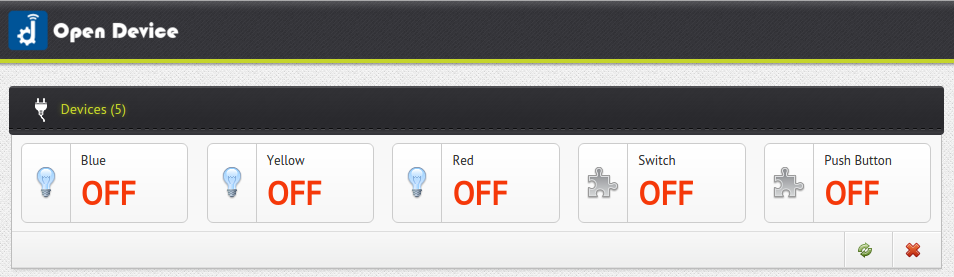
\includegraphics[width=1\linewidth]{Imagens/Cap_4/dashboard-devices}
\par\end{centering}
\caption{Interface de controle de dispositivos\label{fig:dashboard1}}
\end{figure}

\begin{figure}[H]
\begin{centering}
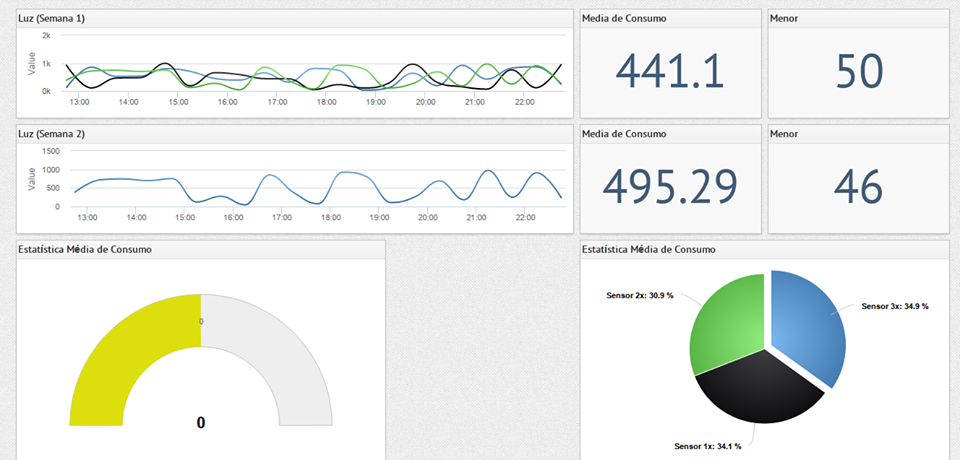
\includegraphics[width=1\linewidth]{Imagens/Cap_4/dashboard-charts}
\par\end{centering}
\caption{Interface de Dashboards Gráficos\label{fig:dashboard2}}
\end{figure}


\section{Serviço de descoberta\label{sec:ServicoDescoberta}}

Conectar e configurar um dispositivo (microcontrolador, sensor ou
atuador), é uma tarefa relativamente simples. Fazer o mesmo para centenas
ou milhares de dispositivos, não é uma tarefa fácil. Este é o cenário
que os pesquisadores e desenvolvedores irão encontrar no ambiente
de Internet das Coisas. Um mecanismo dinâmico, adaptável e utilizando
um processo mais automatizado possível, é necessário para realizar
a descoberta de dispositivos e registro de suas informações básicas.
Além disso existe a necessidade de trabalhar de forma unificada com
diferentes protocolos e dispositivos de rede.

O framework conta com serviços de descoberta de dispositivos, suportando
as tecnologias Usb, Bluetooth, Ethernet e Wi-Fi. O middleware também
disponibiliza um serviço de descoberta, permitindo que as aplicações
clientes o localizem em uma rede local. São dois os possíveis cenários
onde as aplicações e dispositivos IoT estarão executando: Local e
Internet. No cenário onde os dispositivos estão conectados à Internet,
eles devem ser configurados para atuarem como clientes, conectando-se
no servidor em nuvem do OpenDevice em um endereço fixo. Já em um cenário
local, focando-se em dispositivos Ethernet, no cenário de automação
residencial, por exemplo, os dispositivos poderiam atuar em modo cliente
ou como servidor, em ambos os cenários seria necessário configurar
manualmente um IP fixo para cada dispositivo, uma tarefa relativamente
trabalhosa dependendo da quantidade de dispositivos.

Uma solução promissora é o padrão DNS-SD (DNS Service Discovery, RFC
6763) \cite{key-dnssd}, que permite a descoberta de serviços na rede
e associação de um ``DNS local'' para o dispositivo, como por exemplo:
\emph{lampada1.local}. Devido às limitações de alguns hardwares alvos
do estudo (microcontroladores), uma solução mais simples foi adotada.
Trata-se do envio de mensagens UDP em broadcast na rede. Os dispositivos
(hardware) monitoram a rede e ao detectar uma solicitação de descoberta
(um comando do tipo \emph{DISCOVERY\_REQUEST}), enviam uma mensagem
de volta contendo o seu nome, tipo, IP atual, e porta. Desse modo,
todos os dispositivos podem ser configurados com IP dinâmico usando
DHCP, incluindo o próprio servidor (middleware). As aplicações clientes
podem localizar os dispositivos ou middleware utilizando o mesmo mecanismo. 

Foi desenvolvida uma estratégia bastante simples, influenciada pelo
DNS-SD e combinado com a técnica desenvolvida, para conexão com os
dispositivos TCP/IP, usando um endereço com sufixo pré-definido (ex.:
\emph{lampada1}.local.opendevice). A listagem \ref{alg:descoberta}
apresenta um modelo tradicional de descoberta e o modelo usando os
endereços de domínio local. No primeiro exemplo (modelo tradicional)
é obtido o serviço de descoberta e iniciado a busca durante 5 segundos
por dispositivos na rede, em seguida é feita a conexão. No segundo
exemplo, ele permite a simplificação do processo. O endereço informado
``lampada1.local.opendevice'', na verdade não se trata de um domínio,
serve apenas para marcar e iniciar o sistema de descoberta automático,
permitindo uma fácil conexão com determinado dispositivo (hardware).
A imagem \ref{fig:DiagDiscoveryConnect} apresenta um diagrama de
fluxo de como esse processo funciona.

As conexões USB e Bluetooth, possuem mecanismos de descobertas menos
sofisticados, oferecidos pelas próprias implementações no S.O, que
são usados pelo serviço de descoberta. No caso do USB, a classe que
implementa essa conexão (\emph{UsbConnection}), possui o método ``listAvailable'',
que lista todos os dispositivos USB-Serial conectados na maquina.
É possível realizar facilmente uma conexão com o primeiro dispositivo
encontrado usando: \inputencoding{latin9}\lstinline!connect(out.usb())!\inputencoding{utf8}.
A implementação para Bluetooth é similar, onde o método ``listAvailable''
da classe (\emph{BluetoothConnection}), realiza a listagem dos dispositivos
seriais SSP - (Serial Port Profile) disponíveis, também é possível
conectar-se facilmente com o primeiro dispositivo encontrado, usando:
\inputencoding{latin9}\lstinline!connect(out.bluetooth())!\inputencoding{utf8}
(observe que, antes é necessário realizar manualmente o pareamento
dos dispositivos). 

\begin{algorithm}[H]
\inputencoding{latin9}\begin{lstlisting}[language={C++}]
// Modelo tradicional
Set<NetworkDeviceInfo> devices = getDiscoveryService().scan(5000, null);
if(devices.size() > 0){
    NetworkDeviceInfo info = devices.iterator().next();
    if(info.getName().equals("lampada1")) {
        connect(out.tcp(info.getIp() + ":" + info.getPort()));
    }
}

// Modelo usando dom�nio local
connect(out.tcp("lampada1.local.opendevice"));
\end{lstlisting}
\inputencoding{utf8}
\caption{Exemplos de descoberta de dispositivos \label{alg:descoberta}}
\end{algorithm}

\begin{figure}
\begin{centering}
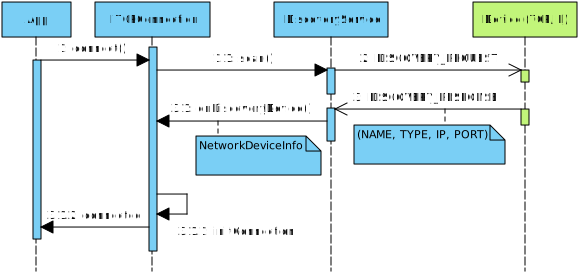
\includegraphics[width=0.8\linewidth]{Imagens/Cap_4/seq_discovery_connect}
\par\end{centering}
\caption{Fluxo de conexão e descoberta\label{fig:DiagDiscoveryConnect}}
\end{figure}


\section{APIs para Aplicações Cliente\label{subsec:ConexoesCliente}}

O conjunto de bibliotecas ou APIs para aplicações clientes, permitem
a rápida construção de aplicações, sem que os pesquisadores ou desenvolvedores
tenham que se preocupar com os detalhes de baixo nível do protocolo,
adotando um modelo orientado a eventos (\emph{Event-Driven}) e usando
orientação a objetos na construção das aplicações, que podem ser aplicações
Web, Desktop, Mobile ou uma interface simulação. O maior desafio encontrado
na construção dessas aplicações é lidar com a heterogeneidade dos
dispositivos (atuadores e sensores), fazer o gerenciamento das conexões
e a integração com a aplicação. A arquitetura disponibiliza um middleware
e um framework para construção aplicações ou middleware customizadas.

As bibliotecas disponibilizadas permitem uma comunicação bidirecional
e são focadas na comunicação em tempo real, dessa maneira é possível
construir gráficos para visualização das informações em tempo-real,
aplicações de simulação, etc. As tecnologias empregadas que permitem
essa comunicação, estão disponíveis para as plataformas Web, Desktop
e Mobile, conforme a tabela \ref{tab:apis-clientes}.

\begin{table}[h]
\begin{centering}
\begin{tabular}{|c|c|c|c|c|}
\hline 
Tipo & Web & Desktop & Mobile (Android) & Alvo de Comunicação\tabularnewline
\hline 
\hline 
USB &  & X &  & Firmware\tabularnewline
\hline 
Bluetooth &  & X & X & Firmware\tabularnewline
\hline 
Socket (TCP) &  & X &  & Middleware/Firmware\tabularnewline
\hline 
WebSocket & X & X & X & Middleware\tabularnewline
\hline 
MQTT &  & X & X & Middleware\tabularnewline
\hline 
\end{tabular}
\par\end{centering}
\caption{APIs Clientes\label{tab:apis-clientes}}
\end{table}


\subsection{Implementação}

A maior parte das bibliotecas são implementados em linguagem Java
com base no framework de conexões (\ref{subsec:Framework-de-Conexoes})
e utilizam o módulo principal (core), que provê as APIs de comandos
e abstração de dispositivos. Porém são disponibilizadas bibliotecas
em JavaScript, apresentada na seção \ref{subsec:SuporteJavaScript},
e Python (experimental). As tecnologias de comunicação (ex.: USB),
são implementadas com auxílio de bibliotecas externas, e suas considerações
são listadas a seguir.

\subsubsection{USB}

A comunicação USB, por utilizar recursos do sistema operacional e
ser dependente da arquitetura, não possui suporte nativo na JVM, apesar
de ser umas das especificações iniciais da plataforma, registrada
sobre a especificação Java USB API (JSR-80)\cite{key-JSR-80}.

Como alternativa, algumas bibliotecas de terceiros foram avaliadas.
Uma das pioneiras e mais utilizadas é a biblioteca RXTX\footnote{https://github.com/rxtx/rxtx}.
Esta biblioteca foi utilizada nas versões iniciais da plataforma,
porém, pelo fato de não ter um desenvolvimento ativo, e nos testes
realizados ter se mostrado instável, apresentando alguns erros (ex.:
problemas de deadlocks e mal funcionamento em plataformas ARM), ela
foi substituída.. A implementação de referência oficial, javax-usb
\footnote{http://javax-usb.sourceforge.net/}, a julgar pelo site
e documentação, estão abandonados há muito tempo.

A implementação utilizada, foi baseada na biblioteca JSSC (Java Simple
Serial Connector)\footnote{https://github.com/scream3r/java-simple-serial-connector},
que oferece suporte para várias plataformas\footnote{Segundo o site: Windows(x86, x86-64), Linux(x86, x86-64, ARM soft
\& hard float), Solaris(x86, x86-64), Mac OS X(x86, x86-64, PPC, PPC64)}, se mostrando uma alternativa promissora. Ela é a biblioteca utilizada
na IDE do Arduino, substituindo a RXTX em versões anteriores.


\subsubsection{Bluetooth}

A comunicação Bluetooth é apoiada na especificação Java JSR-82\cite{key-JSR-82},
possui implementações bem estabelecidas e estáveis para o desenvolvimento
para dispositivos móveis, usando JavaME. As implementações para ambiente
desktop, sofrem com os mesmos problemas de plataforma do USB. Uma
das poucas alternativas, é a biblioteca BlueCove\footnote{http://bluecove.org/},
que tem implementações para os principais sistemas operacionais (Windows,
Linux, MacOS). Para o suporte à plataformas ARM (no RaspberryPi),
foi necessário a recompilação da mesma e ajustes, pois não foram encontradas
versões disponibilizadas no site oficial nem de terceiros. 

As implementações para aplicações mobile, estão disponíveis para o
Android, e utiliza as APIs disponibilizadas pela própria plataforma.
A arquitetura do OpenDevice, é projetada de maneira que a implementação
utilizada é transparente para o desenvolvedor, sem precisar de modificações
no código.

\subsubsection{Socket (TCP)}

Foi implementada usando as APIs nativas do Java, usando as classes
da API de Socket. Devido o Java ser projetado para construção de sistemas
em rede, as APIs de comunicação são suportadas em praticamente todas
as plataformas.

Apesar de ser compatível com as plataformas mobile (Android), a implementação
atual não é indicada, por não levar em consideração requisitos de
consumo de bateria.

\subsubsection{WebSocket}

A implementação de WebSocket para plataforma Web utiliza as próprias
APIs disponibilizadas pelos navegadores, através da implementação
da especificação de WebSocket para o HTML5\cite{key-ws-1,key-ws-2}.

A implementação para aplicações Desktop e Mobile(Android), são baseadas
na biblioteca wAsync\footnote{https://github.com/Atmosphere/wasync}.
As especificações da API de WebSocket para plataforma Java, estão
disponíveis através da especificação JSR 356\cite{key-JSR-356}, e
uma implementação de referência chamada Tyrus\footnote{https://tyrus.java.net/},
se mostra promissora, porém ainda conta com limitações para utilização
no Android e por conta disso não foi utilizada.


\section{Armazenamento\label{sec:Armazenamento}}

O sistema de armazenamento guarda informações sobre as conexões, dispositivos
e histórico de dados. A implementação padrão é baseada em um banco
de dados orientado a grafos, chamado Neo4j\footnote{http://www.neo4j.com},
baseado no conceito NoSQL, que permite ser executado de forma embarcada,
junto com a aplicação. A base da arquitetura do Neo4j é construída
usando o framework Netty, o mesmo utilizado nas implementações dos
módulos de servidores (\ref{subsec:ConexoesServidores}), permitindo
otimizando alguns recursos de espaço e consumo de memória. Ao incluir
o middleware e o módulo de interface gráfica, as informações sobre
os \emph{dashboards} e configuração dos gráficos também são armazenadas.
Na construção de aplicações e protótipos, o sistema de armazenamento
pode ser dispensado, usando apenas o sistema de cache de dispositivos,
porém este não permite a visualização de dados históricos. 


\section{Firmware\label{subsec:Arquitetura-do-Firmware}}

O firmware é um componente que permite a criação de dispositivos (coisas)
para Internet das Coisas. Ele foi projetado para criação de sistemas
embarcados para microcontroladores, e se baseia na API do Arduino
para acesso aos periféricos do microcontrolador. Apesar de utilizar
a API do Arduino, ele não está limitado apenas aos \emph{hardwares}
denominados Arduino. Várias outras plataformas vem implementando o
suporte a sua API\cite{arduino-comp1,arduino-comp3}, como por exemplo
o ESP8266\cite{url:esp8266:espressif}, um SoC (System-On-Chip) de
32 bits com Wi-Fi embutido. Hardwares com maior poder de processamento
e que suportem a execução na JVM (Máquina Virtal Java), não farão
utilização do firmware.

O firmware é flexível e pode ser utilizado como base para criação
sistemas embarcados customizados, dando suporte a várias tecnologias
de comunicação, como: Usb, Bluetooth, Ethernet e Wi-Fi, que pode operar
tanto no modo cliente como no modo servidor (vide tabela \ref{tab:FirmwareConexoes}).
Dentro da plataforma do Arduino ele é disponibilizado como uma biblioteca
escrita em C++, e é responsável pelo gerenciamento dos dispositivos,
conexões e implementa o protocolo do OpenDevice. 


\subsection{Visão Geral}

Na figura \ref{fig:ArquiteturaFirmware} é apresentada uma visão geral
de como a arquitetura do \emph{firmware} está estruturada. Podemos
observar que ela é similar a arquitetura geral do projeto (Figura
\ref{fig:Arquitetura}), a camada central, que compreende o firmware,
é a junção das bibliotecas do Arduino, APIs do OpenDevice e o código
do usuário (\emph{User Code}), que auxiliam na criação dos sistemas
embarcados. A camada superior, compreende as aplicações cliente, que
implementam os protocolos de baixo nível (\ref{subsec:Protocolo}),
com auxílio das bibliotecas disponibilizadas pelo OpenDevice.

\begin{figure}
\begin{centering}
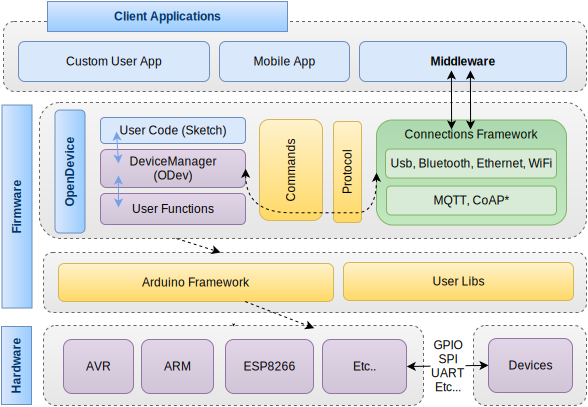
\includegraphics[width=1\linewidth]{Imagens/Cap_4/arquitetura-firmware}
\par\end{centering}
\caption{Arquitetura do Firmware\label{fig:ArquiteturaFirmware}}
\end{figure}


\subsection{Meios de comunicação suportados}

A tabela \ref{tab:FirmwareConexoes} apresenta as tecnologias de comunicação
que são suportadas, destacadas juntos com os modelos de comunicação.
Entende-se por modelo de comunicação a forma como o firmware irá operar,
se é no modo cliente ou no modo servidor.

\begin{table}[h]
\begin{centering}
\begin{tabular}{|c|c|c|}
\hline 
Tipo & Cliente & Servidor\tabularnewline
\hline 
\hline 
Usb & Não & Sim\tabularnewline
\hline 
Bluetooth & Não & Sim\tabularnewline
\hline 
Ethernet & Sim & Sim\tabularnewline
\hline 
Wi-Fi & Sim & Sim\tabularnewline
\hline 
\end{tabular}
\par\end{centering}
\caption{Comunicação suportada pelo firmware\label{tab:FirmwareConexoes}}

\end{table}


\subsection{Gerenciamento de conexões\label{subsec:FirmwareGerenciamentoConn}}

O bloco denominado ``Connections Framework'', trata-se de adaptações
das bibliotecas disponibilizadas pelo Arduino (``User Libs'' e nativas)
para implementação das conexões, usando seus respectivos módulos módulos
(shields), permitindo assim a comunicação com o middleware e aplicações.
Por exemplo, o suporte a conexões Ethernet usando o módulo ENC28J60,
necessita de uma biblioteca específica que realiza a implementação
do protocolo TCP/IP via software, já o modulo(shield) Ethernet baseado
no chip W5100 é suportado nativamente pelo framework do Arduino e
OpenDevice. O Arduino disponibiliza uma API base para implementação
das conexões Ethernet e Wi-Fi. Módulos (shields) que implementem essa
API estariam compatíveis automaticamente com o OpenDevice. 

As conexões USB e Bluetooth, são comunicações seriais, acessíveis
através de portas UART, referenciadas geralmente pelas variáveis
\emph{Serial}, \emph{Serial1}, etc. E que têm como implementação base
a classe \emph{Stream}(do Arduino). Outras tecnologias de conexão,
que se baseiem nos mecanismos apresentados acima serão automaticamente
suportados, ou necessitariam de pequenos ajustes. 

As tecnologias implementadas estão listadas na tabela \ref{tab:FirmwareConexoes}
e mais adiante na seção de hardwares testados (\ref{par:Hardwares-Testados});

\subsection{Gerenciamento dos dispositivos}

No firmware é realizado o mapeamento dos dispositivos e seus respectivos
IDs para os pinos do microcontrolador. Ele interpreta os comandos
enviados pelas aplicações e as transforma em ações. Um exemplo de
mapeamento dos dispositivos é demonstrado da listagem \ref{alg:firmware1},
onde é feita a configuração de forma estática, adicionando atuadores
e sensores. As classes que abstraem os dispositivos existem, e são
baseados na classe Device, e conta com um atributo do tipo \emph{booleano}
chamado \textquotedbl{}sensor\textquotedbl{}, para identificar se
é um atuador ou sensor. 

\begin{algorithm}[H]
\inputencoding{latin9}\begin{lstlisting}[language={C++}]
#include <OpenDevice.h>
// Mapeamento dos Dispositivos
void setup(){
	ODev.name("ODev-Thing1");
    ODev.addCommand("alertMode", alertMode);
    ODev.addDevice(5, Device::DIGITAL); // ID:1
    ODev.addSensor(3, Device::DIGITAL); // ID:2 
    ODev.addSensor(RFIDSensor(10,9)); // ID:1
    ODev.begin();
}

void loop(){
  ODev.loop();
}
// Comando de Usuario
void alertMode(){
  ODev.debug(ODev.readString());
  int count = ODev.readInt();
  // ....
}
\end{lstlisting}
\inputencoding{utf8}
\caption{Exemplo de configuração do firmware\label{alg:firmware1}}
\end{algorithm}


\subsubsection{Dispositivos suportados}

A tabela \ref{tab:FirmwareDevices}, apresenta a lista de dispositivos
suportados nativamente. A extensão de dispositivos permite a inclusão
e suporte de novos dispositivos, sendo apresentado com mais detalhes
na seção \ref{subsec:FirmwareExtensibilidade}.

\begin{table}[h]
\begin{centering}
\begin{tabular}{|c|c|c|}
\hline 
Nome & Tipo & Biblioteca Extra\tabularnewline
\hline 
\hline 
Genérico Digital (1 pino) & Atuador / Sensor & Não\tabularnewline
\hline 
Genérico Analógico (1 pino) & Atuador / Sensor & Não\tabularnewline
\hline 
RFID (MFRC522) & Sensor & Sim\tabularnewline
\hline 
Servo Motor & Atuador & Não\tabularnewline
\hline 
Temperatura (LM35) & Sensor & Não\tabularnewline
\hline 
Infra-Vermelho (Emissor) & Atuador & Sim\tabularnewline
\hline 
Infra-Vermelho (Receptor) & Sensor & Sim\tabularnewline
\hline 
\end{tabular}
\par\end{centering}
\caption{Dispositivos suportados nativamente\label{tab:FirmwareDevices}}
\end{table}


\subsection{Comandos de Usuário}

Os desenvolvedores podem criar novos comandos, estendendo o protocolo
ou usando os recursos de comandos do usuário (\emph{User Functions},
na figura \ref{fig:ArquiteturaFirmware}). Esse recurso permite criar
novos comandos e vinculá-los à funções definidas pelo próprio usuários.
A listagem \ref{alg:firmware1}, apresenta um exemplo desse recurso.
Os comandos são criados usando a função ``\inputencoding{latin9}\lstinline!ODev.addCommand!\inputencoding{utf8}'',
definindo o nome e a função que será executada ao receber esse comando.
No lado da aplicação (Java), esse comando é executado através do método:
``\inputencoding{latin9}\lstinline!sendCommand("alertMode","Your String", 5)!\inputencoding{utf8}''.
Observe que também é possível passar parâmetros para a função, e no
lado do firmware os parâmetros podem ser recuperados usando as funções
``\inputencoding{latin9}\lstinline!ODev.read*()!\inputencoding{utf8}''.

\subsection{Mecanismos de leitura de sensores\label{subsec:FirmwareLeituraSensores}}

O mecanismo de leitura adotado, também é um sistema baseado em eventos,
ou seja, as aplicações não precisam realizar consultas para obter
os valores dos sensores. Quando houver alguma alteração no valor do
sensor, automaticamente o firmware envia o valor atualizado para as
aplicações. Internamente, o mecanismo de leitura opera de dois modos:
síncrono e assíncrono, que serão apresentados a seguir.

\subsubsection{Modo Síncrono (Polling)}

O mecanismo síncrono ou ``polling'', é o mecanismo ativo por padrão,
e por ser uma implementação mais simples, pode ser utilizado em qualquer
microcontrolador, porém existem algumas limitações. Por se tratar
de um mecanismo onde é preciso realizar uma leitura de todos os sensores(pinos)
configurados, e comparar o valor lido com o valor atual, algum tempo
será perdido lendo sensores que não alteraram seu valor, e consumindo
recursos desnecessários CPU, que poderia estar desempenhando outras
atividades. Dependendo do tempo da leitura dos sensores, alguma informação
importante pode ser perdida. A leitura de pinos digitais e analógica
é bem rápida, a leitura de um pino analógico por exemplo, demora cerca
de 100 microssegundos~(0.0001 s), em um processador AVR 8-bits\footnote{https://www.arduino.cc/en/Reference/analogRead}.

\subsubsection{Modo Assíncrono (Interrupções)}

As interrupções são sinais enviados para o microcontrolador com eventos
que precisam de imediata atenção. A interrupção permite que o processador
interrompa a tarefa atual , salve seu contexto, e execute um rotina
especial de interrupção, conforme na figura \ref{fig:interrupcoes}.
Quando um dispositivo precisa de atenção ele envia um sinal para o
processador que desloca a execução para rotina de interrupção (ISR).
O suporte a interrupção externas (mudança nos pinos de I/O), depende
do microcontrolador, alguns suportam interrupções em todos os pinos
e outros suportam interrupções apenas em alguns pinos predefinidos.
Para citar exemplos, o Arduino DUE (SAM3X8E ARM) possui suporte a
interrupções externas em todos os pinos, já o Arduino Uno (e similares
com chip ATmega328p) suporta interrupções externas apenas nos pinos
2 e 3. 

Para lidar com as limitações encontradas, o firmware utiliza uma biblioteca\footnote{https://github.com/GreyGnome/EnableInterrupt}
que permite habilitar a associação de rotinas de interrupções individuais
para todos os pinos do microcontrolador, fazendo o gerenciamento do
estado dos pinos. Algumas limitações também são encontradas nessa
alternativa. O tempo de interrupção pode sofrer atrasos na ordem de
alguns micro-segundos para pinos que não suportem nativamente as interrupções
externas. Dependendo da aplicação isso pode ser relevante. Uma análise
realizada dos tempos de tratamento das interrupções, nessa implementação,
é apresentada em \cite{key-isr}.

Para habilitar o suporte a interrupções em um sensor é preciso habilitar
o recurso nas configurações gerais e ativar os sensores que serão
lidos com base nas interrupções. Com base no exemplo da listagem \ref{alg:interrupcoes},
quando ocorre alguma interrupção nos sensores configurados, os valores
deles são lidos pela rotina \emph{``OpenDeviceClass::onInterruptReceived()}'',
e marcados para sincronização, que irá ocorrer no ciclo de ``loop''.
Um ponto importante é que os dados não podem ser enviados na rotina
de interrupção, pois ela deve ocorrer o mais rápido possível, evitando
problemas na leitura de outras interrupções e podem ocasionar conflitos
com as interrupções de leituras das portas seriais. Detalhes de execução
desse fluxo serão apresentados na seção \ref{subsec:LeituraSensores}.

\begin{algorithm}[H]
\inputencoding{latin9}\begin{lstlisting}[language={C++}]
#include <EnableInterrupt.h>
#include <OpenDevice.h>

void setup() {
  // Modo 1
  ODev.addSensor(3, Device::DIGITAL)->enableInterrupt(CHANGE); // ID:1
  // Modo 2
  Device *s2 = ODev.addSensor(4, Device::DIGITAL); // ID:2
  *s2->enableInterrupt(CHANGE);
  
  ODev.begin();
}

void loop() {
  ODev.loop();
}
\end{lstlisting}
\inputencoding{utf8}
\caption{Leitura usando interrupções (Arduino/C++) \label{alg:interrupcoes}}
\end{algorithm}

\begin{figure}
\begin{centering}
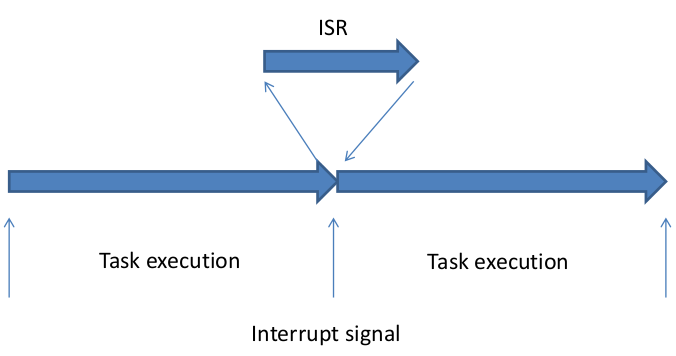
\includegraphics[width=1\linewidth]{Imagens/Cap_4/firmware_interrupcao}
\par\end{centering}
\caption{Execução de uma interrupção\label{fig:interrupcoes}}
\end{figure}


\subsection{Configuração dinâmica e parametrizações\label{subsec:ConfiguracaoDinamica}}

O firmware tenta detectar o hardware e as bibliotecas utilizadas e
realizar as parametrizações necessárias, necessitando o mínimo de
configurações possíveis. Um exemplo da técnica é apresentado na listagem
\ref{alg:firmware2}, onde a implementação da Ethernet é alterada
apenas escolhendo o \emph{``include''} correspondente, sem necessidade
de alterações no código. As duas implementações são totalmente diferentes,
porém essas diferenças são abstraídas pelo firmware, permitindo que
o desenvolvedor foque na lógica do sistema.

Algumas parametrizações e valores padrão, como velocidade, portas,
tamanhos dos \emph{buffers} de recepção de dados, podem ser ajustados
no arquivo: ``config.h'', bem como é possível habilitar o modo de
depuração (debug), para auxiliar na detecção de algum erro que esteja
ocorrendo. As informações de depuração podem ser direcionadas para
a conexão atual ou para uma porta serial do microcontrolador.

\begin{algorithm}[H]
\inputencoding{latin9}\begin{lstlisting}[language={C++}]
//#include <UIPEthernet.h> // ENC28J60
#include <Ethernet.h>
#include <OpenDevice.h>

void setup(){
  ODev.addDevice(13, Device::DIGITAL);
  ODev.begin();
}

void loop(){
  ODev.loop();
}
\end{lstlisting}
\inputencoding{utf8}
\caption{Exemplo de configuração do firmware\label{alg:firmware2}}
\end{algorithm}


\subsection{Monitoramento}

O sistema de monitoramento permite informar às aplicações a utilização
da memória RAM e EPROM do microcontrolador e monitorar os estados
das conexões, utilizando um mecanismo de Keep-Alive / Heartbeat. Em
algumas situações pode ocorrer que algumas das partes da comunicação
fique fora de sincronia, devido a problemas no link, falhas de software
ou hardware. Esse estado é geralmente chamado conexão semi-aberta
(half-open connection). É importante que o lado da conexão que está
funcionando corretamente seja notificado ou detecte a falha da outra
ponta, e tente uma reconexão ou fecha a conexão semi-aberta. Mesmo
existindo mecanismos similares em alguns protocolos como o TCP/IP,
ele pode não ser ideal para alguns tipos de aplicações, pois em média
ele é executado em um intervalo de duas horas e não permite ajustes
a nível de aplicações, necessitando de ajustes no sistema operacional\cite{key-keepa}.
Por outro lado, outras conexões (ex.: USB) não suportaram este mecanismo.
Para contornar esses problemas, o recurso de Keep-Alive / Heartbeat
foi implementado no firmware. Quando é habilitado o suporte ao protocolo
MQTT, o mecanismo de Keep-Alive do próprio protocolo são utilizados.

Este mecanismo é implementado através do envio de comando do tipo
PING, em um intervalo ajustável e aguardando seu retorno através do
comando do tipo PING\_RESPONSE, podendo ser habilitado e desabilitado
conforme a necessidade. Ao detectar uma falha ou estouro do tempo
determinado (time-out), a aplicação ou middleware decide o que fazer
com a conexão em estado inválido, se tenta uma reconexão ou finaliza
a conexão, liberando os recursos alocados.


\subsection{Extensibilidade\label{subsec:FirmwareExtensibilidade}}

O firmware é projetado como uma biblioteca, permitindo aos desenvolvedores
facilmente customizar e criar seu próprio firmware através da inclusão
do código de usuário (Sketch, vide figura \ref{fig:ArquiteturaFirmware}).
O mecanismo de conexões (Connections Framework) também é flexível,
permitindo plugar novas conexões facilmente, através da extensão da
classe \emph{DeviceConnection}, ou através do mecanismo de ``Custom
Connections'', que permite a criação de novas conexões, sobrescrevendo
métodos predefinidos usando apenas arquivos de cabeçalho (.h). Mais
detalhes serão apresentados a seguir.

A classe Device pode ser estendida para dar suporte a dispositivos
(sensores ou atuadores) mais complexos, que utilizem mais de um pino
ou trabalhem com um protocolo específico (ex.: SPI, OneWire). Um exemplo
de especialização desta classe é realizado pele classe \emph{RFIDSensor},
disponível nas bibliotecas do firmware, que permite a integração de
um sensor RFID de proximidade (baseado no chip MFRC522). A inclusão
de novos dispositivos, é realizada estendendo a classe Device e implementando
os métodos ``setValue'' e ``hasChanged''. 

Outro método de inclusão de novos dispositivos, mais especificamente
sensores, permite a integração com sensores mais complexos (que utilizem
um protocolo específico), de uma forma simplificada e sem a necessidade
de estender a classe Device, facilitando assim a integração e testes.
A listagem \ref{alg:firmware-newsenor} apresenta um exemplo deste
recurso, onde a leitura do sensor é implementada por um método definido
pelo usuário no programa principal (Sketch), onde o método deve retornar
a leitura do sensor. O firmware é responsável por executar esse método
e verificar se houve alguma mudança no valor do sensor, caso exista
alguma alteração, as aplicações são notificadas.

\begin{algorithm}[H]
\inputencoding{latin9}\begin{lstlisting}[language={C++}]
void setup(){
    ODev.addSensor(readRfid); // ID:1
    // ... sensor setup ...
    ODev.begin();
}

unsigned long readRfid(){
  // sensor logic
}
\end{lstlisting}
\inputencoding{utf8}
\caption{Suporte a novos sensores\label{alg:firmware-newsenor}}
\end{algorithm}


\subsubsection{Mecanismo ``Custom Connections''}

Nativamente o \emph{firmware} suporta qualquer conexão que estenda
a classe \emph{Stream} (do Arduino). Caso seja necessário a inclusão
de outro mecanismo de comunicação, onde a biblioteca projetada para
o mesmo não implemente a classe Stream, um ``adaptador'' pode ser
criado para essa conexão. Exemplos dessa implementação são encontrados
no próprio firmware (arquivo: EthernetServerConnection.h) e a estrutura
básica é apresentada na listagem \ref{alg:firmware-custconn}. A vantagem
é que não é necessária a criação de classes (C++), necessitando apenas
de um arquivo de cabeçalho (.h). Ao realizar a inclusão deste cabeçalho
no programa, o firmware automaticamente detecta que deve ser usado
essa conexão e realiza as chamadas dos métodos implementados. É importante
que a classe retornada pelo método ``\_loop()'', seja uma instância
e estenda a classe ``Stream'' para que o mecanismo funcione. 

\begin{algorithm}[H]
\inputencoding{latin9}\begin{lstlisting}[language={C++}]
#define USING_CUSTOM_CONNECTION 1
#define CUSTOM_CONNECTION_CLASS YourClassExtendStream

void custom_connection_begin(){
  
}

CUSTOM_CONNECTION_CLASS custom_connection_loop(DeviceConnection *conn){
  return // return instance of YourClassExtendStream;
}

\end{lstlisting}
\inputencoding{utf8}
\caption{Exemplo do mecanismo ``Custom Connections'' \label{alg:firmware-custconn}}
\end{algorithm}


\section{Fluxo de Mensagens\label{subsec:FluxoMensagens}}

Nesta seção abordamos os principais fluxos de execução, encontrados
no firmware, middleware e aplicações, auxiliando a entender o processo
interno de execução e quais componentes são utilizados em cada etapa.

\subsection{Envio de Comandos\label{subsec:FluxoEnvioComandos}}

A figura \ref{fig:seq_command_send}, apresenta o fluxo de envio de
comandos entre uma aplicação, que se comunica diretamente com os dispositivos
(firmware). A primeira etapa inicia com a abstração do dispositivo
e a execução do seu método ``on'' ou ``setValue'' (ex.: led.on()).
Esse método gera um evento que é capturado pelo framework (fluxo 1),
através da classe \emph{DeviceManager}, que cria o comando apropriado,
no caso o \emph{DeviceCommand}, e inicializa com as informações do
ID do dispositivo, tipo (ANALOG ou Digital) e valor e repassa para
o CommandDelivery (fluxo 1.2), que cuida do envio para as conexões
de saída de modo assíncrono, usando a \emph{SendTask}. As mensagens
são serializadas para o formato do protocolo (\ref{subsec:Protocolo})
do OpenDevice usando o \emph{MessageSerializer}. Cada comando enviado,
recebe um ID (TrackingID), que é gerenciado pelo CommandDelivery,
e é usado para fazer o mapeamento dos comandos enviados e comandos
recebidos (fluxo 2 e 3). O ID do comando é gerado de forma sequencial,
até um limite estabelecido pelo protocolo, depois é reiniciado a contagem.
A SendTask, é registrada para receber os eventos das conexões. Quando
a resposta é recebida pela conexão, o método ``onMessageReceived''
(fluxo 3) é executado, e a resposta é mapeada para o comando enviado.

\begin{figure}[h]
\begin{centering}
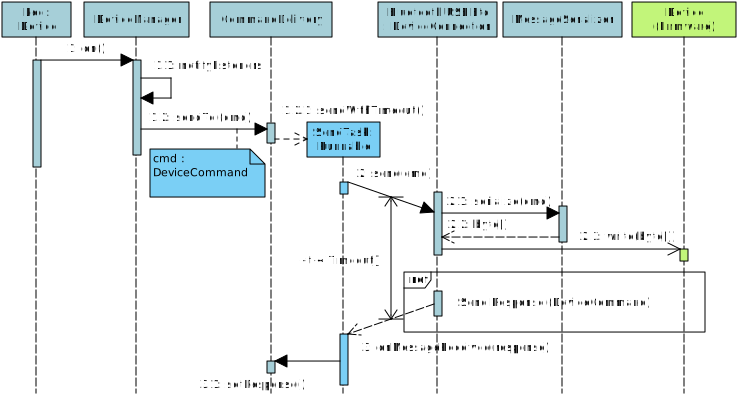
\includegraphics[width=1\linewidth]{Imagens/Cap_4/seq_command_send}
\par\end{centering}
\caption{Envio de Comandos\label{fig:seq_command_send}}
\end{figure}


\subsection{Processamento dos Comandos (Dispositivo)}

A figura \ref{fig:seq_firmware_read}, demonstra o fluxo de execução
do firmware, para realizar a leitura dos comandos das aplicações (ou
do middleware), transforma-lo em ações reais.

Os comandos recebidos são tratados por uma implementação da classe
\emph{Stream} (fluxo 1), que pode ser uma implementação nativa do
Arduino, como a \emph{Serial} ou \emph{EthernetClient}, ou uma implementação
disponibilizada por uma biblioteca de terceiros, que implementa outra
tecnologia de comunicação. Geralmente esses dados são armazenados
em um buffer, de software ou de hardware, e serão lidos no ciclo de
``loop'' do programa principal, através da chamada do ``checkDataAvailable''
(fluxo 2), que ao identificar o final da mensagem especificado no
protocolo, faz a desserialização através do método ``parseCommand''
( fluxo 2.3), e repassa para a classe principal da biblioteca do OpenDevice
(fluxo 2.4), que verifica que tipo de comando foi recebido e faz o
tratamento adequado. Caso a mensagem recebida (fluxo 2.4), seja um
\emph{DeviceCommand} (Ex.: Analogic ou Digital), o dispositivo relacionado
é localizado através do ``DeviceID'', e em seguida seu valor é alterado
(fluxo 3), conforme o valor recebido pelo comando. Em seguida a implementação
do Device determina como será o tratamento para o valor recebido.
Por exemplo, se o dispositivo for um dispositivo do tipo DIGITAL,
a implementação chama o método ``digitalWrite'' da API do Arduino,
caso seja um Device do tipo ANALOG, a implementação chama o método
``analogWrite''.

Quando um comando é recebido com sucesso e o dispositivo relacionado
é encontrado, uma resposta é enviada para a aplicação (fluxo 4.1.1),
informando o estados da execução. Essa resposta é encapsulada através
da classe \emph{ResponseCommand}, podendo ter vários status, conforme
a tabela \ref{tab:CommandStatusResp}, na seção referente ao protocolo
(\ref{subsec:Protocolo}).

\begin{figure}[h]
\begin{centering}
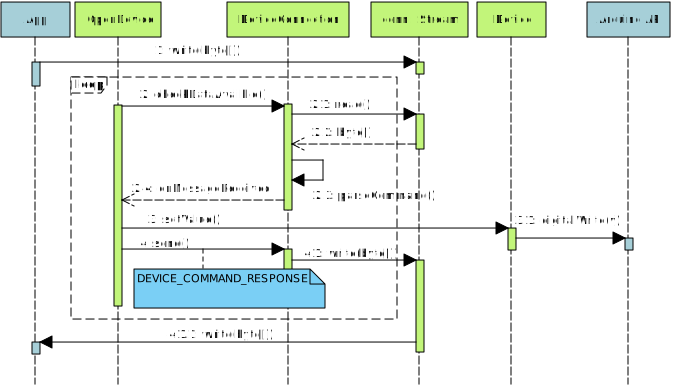
\includegraphics[width=1\linewidth]{Imagens/Cap_4/seq_firmware_read}
\par\end{centering}
\caption{Processamento dos Comandos\label{fig:seq_firmware_read}}
\end{figure}


\subsection{Recebimento de Comandos}

O diagrama de sequência apresentado na figura \ref{fig:seq_send_response},
trata-se da continuação do fluxo, quando o dispositivo (firmware)
devolve a resposta com o status da execução do comando para a aplicação
ou middleware. O componente que fará a leitura dos dados brutos, depende
da implementação da conexão. No exemplo da figura, foi utilizando
um \emph{StreamReader}, mais especificamente \emph{CommandStreamReader},
que é a implementação base para lidar com as conexões implementados
no módulo \noun{connection-stream} (USB e Bluetooth por exemplo).
Essa implementação em específico, utiliza uma ``thread'' para leitura
dos dados de cada conexão, e ao identificar o recebimento do pacote
completo, ele notifica a conexão (fluxo 1.3), que por sua vez notifica
os componentes interessados (fluxos 2 e 3).

Quando se trata de uma resposta de um comando, por exemplo DeviceCommand,
a SendTask, criada e gerenciada pelo CommandDelivery, é notificada
e atualiza o status do comando que foi enviado, com base do ID do
comando (TrackingID) e faz a liberação (remove a trava) do comando.

Caso não seja uma resposta de um comando, por exemplo a leitura de
um sensor, o CommandDelivery não é utilizado . O responsável por tratar
esse comando é o DeviceManager, como será visto na seção seguinte
(\ref{subsec:LeituraSensores}).

\begin{figure}[h]
\begin{centering}
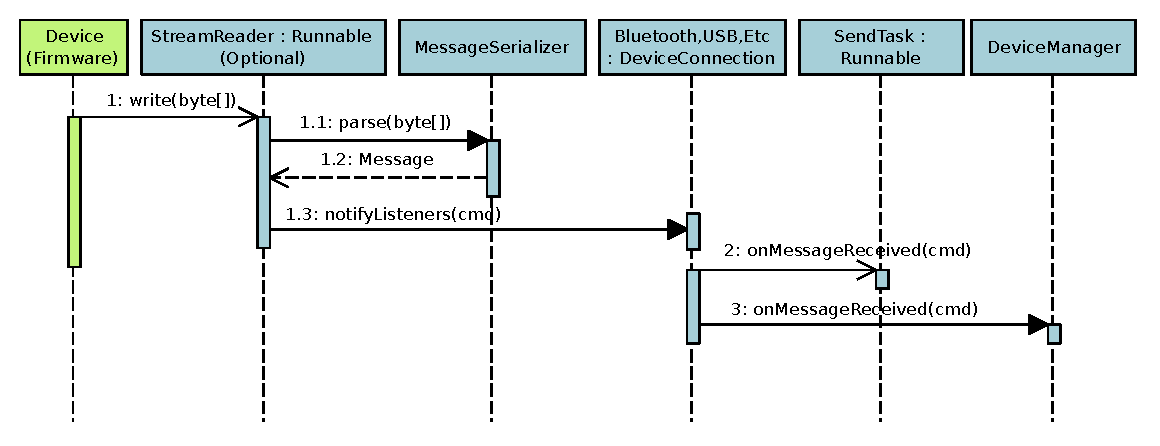
\includegraphics[width=1\linewidth]{Imagens/Cap_4/seq_send_response}
\par\end{centering}
\caption{Recebimento de Comandos\label{fig:seq_send_response}}
\end{figure}


\subsection{Leitura de Sensores\label{subsec:LeituraSensores}}

O fluxo da leitura de sensores, apresentados nas figuras \ref{fig:seq_firmware_read_poll}
e \ref{fig:seq_firmware_read_interrupt}, trata-se também de um fluxo
de recebimento de comandos, é similar ao da figura \ref{fig:seq_send_response}.
Como abordamos na seção \ref{subsec:FirmwareLeituraSensores}, o sistema
de leitura de sensores é implementado de dois modos: síncrono (polling)
e assíncrono (interrupções). O modo utilizado depende do suporte que
o \emph{hardware.} Como exemplo, utilizamos um microcontrolador AVR~8Bits~(ex.:
Arduino), executando o firmware, e enviando os dados dos sensores
para a aplicação (ou middleware).

\subsubsection{Leitura Síncrona (Polling)}

No modo síncrono, a leitura dos sensores é feito no ``loop'' principal,
e é realizada pela classe \emph{OpenDevice}, através do método ``checkSensorsStatus()''
(fluxo 1). Neste método todos os sensores serão lidos de forma sequencial,
através do método ``hasChanged()'' da classe Device. Ao executar
esse método o valor do dispositivo é atualizado, e caso tenha sofrido
alguma alteração (fluxo 1.1.2), um comando (\emph{DeviceCommand})
com o ID do dispositivo e valor lido é enviado para ao conexão (fluxo
1.2), que cuida de serializar e enviar os dados para a aplicação.

\begin{figure}[h]
\begin{centering}
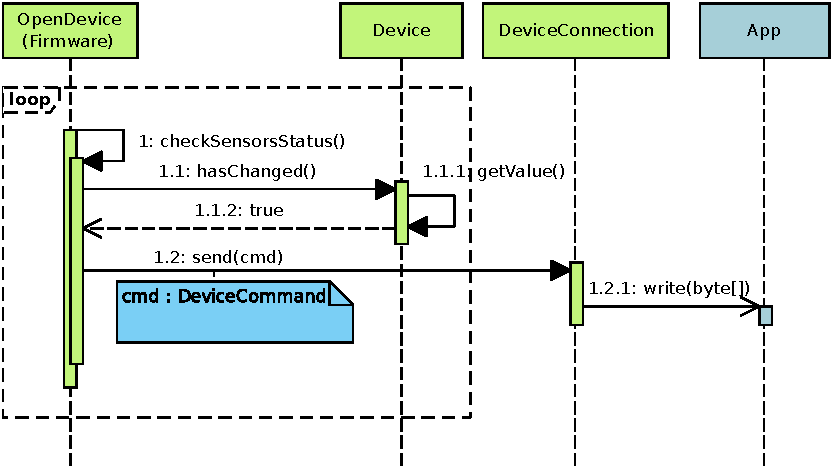
\includegraphics[width=1\linewidth]{Imagens/Cap_4/seq_firmware_read_poll}
\par\end{centering}
\caption{Leitura de Sensores no modo Polling\label{fig:seq_firmware_read_poll}}
\end{figure}


\subsubsection{Leitura Assíncrona (Interrupções)}

O método de leitura assíncrona, apresentado na figura \ref{fig:seq_firmware_read_interrupt},
é realizado através de interrupções, como mencionamos na seção \ref{subsec:FirmwareLeituraSensores}.
Quando habilitado o suporte a interrupções, a classe OpenDevice é
registrada para receber as interrupções através do método ``onInterruptReceived()''.
Neste método o dispositivo correspondente ao pino que sofreu a interrupção
é localizado, e seu valor é atualizado. Os dispositivos que sofrerem
alterações nos seus valores durante a interrupção, são marcados para
sincronização (fluxo 1.2), que irá ocorrer na próxima execução do
“loop” principal do programa. Similar à leitura síncrona, o método
``checkSensorsStatus()'' é chamada no ``loop'', porém neste caso
não é feito nenhuma leitura dos pinos, apenas o envios das informações
para dos dispositivos que sofreram alterações para a aplicação (fluxo
1.2 e 2.1). A vantagem neste caso é que enquanto estão sendo enviadas
as informações para aplicação, caso algum dispositivo tenha seu valor
alterado, a interrupção cuida de deslocar o fluxo de execução, salvar
esse valor e retornar para a serialização dos dados. Na implementação
no modo síncrona (polling), esse valor seria perdido.

\begin{figure}[h]
\begin{centering}
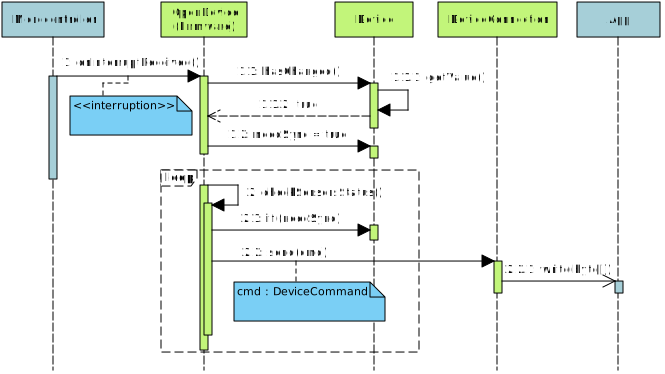
\includegraphics[width=1\linewidth]{Imagens/Cap_4/seq_firmware_read_interrupt}
\par\end{centering}
\caption{Leitura de Sensores usando Interrupções\label{fig:seq_firmware_read_interrupt}}
\end{figure}


\subsection{Envio de Comandos (Aplicação - Middleware - Dispositivo)}

A figura \ref{fig:seq_send_ws}, apresenta o fluxo de execução de
um comando enviado por uma aplicação cliente (WebApp) para os dispositivos,
através do middleware. O framework trabalha com dois conceitos de
conexões: (1) conexões de entrada, ou seja, os servidores e (2) conexões
de saída, geralmente as conexões com os dispositivos físicos. O componente
representado em ``WSServerConnection'', é um servidor WebSocket
disponibilizado pelo módulo \noun{rest-ws-server, }que atua como uma
conexão de entrada. A aplicação web no exemplo, está utilizando a
biblioteca \noun{opendevice-js}, uma das implementações de cliente
usando WebSocket, permitindo a conexão de forma simples com o servidor,
e oferecendo a abstração dos dispositivos para a camada Web.

Ao alterar o valor de algum dispositivo na camada Web, que pode ser
através dos métodos nos objetos JavaScript (fluxo 2), ou através de
métodos disponibilizados no \noun{opendevice-js}, um comando é enviado
via WebSocket para o Middleware (fluxo 2.1). A representação da conexão
com o cliente ``WSResource'' recebe o comando (fluxo 2.1.1) e notifica
para o DeviceManager (fluxos 2.1.2 e 2.1.2.1), que faz a atualização
do dispositivo relacionado ao comando recebido, salva no histórico
de alterações, e repassa o comando para os dispositivos físicos através
das conexões de saída. O procedimento de envio, representado na imagem
pelo bloco ``Ref: Send Command'', é o mesmo procedimento realizado
no fluxo apresentado na seção Envio de Comandos (\ref{subsec:FluxoEnvioComandos}).

O recebimento da resposta do dispositivo físico (fluxo 3), é redirecionado
para a conexão de origem (WSResource). O redirecionamento é feito
baseado na identificação da conexão (UUID), que é gerado no momento
de sua criação (fluxo 1.1.1), e o mesmo é associado ao comando quando
ele é enviado ou recebido, sendo então possível enviar a resposta
para o cliente correto. Deste modo é possível permitir que múltiplas
aplicações acessem o mesmo dispositivo, contornando as limitações
do USB e Bluetooth que permitem apenas um cliente, ou mesmo de conexões
Ethernet ou Wi-Fi, que dependendo do hardware, podem suportar apenas
um cliente ou um número limitado.

\begin{figure}[h]
\begin{centering}
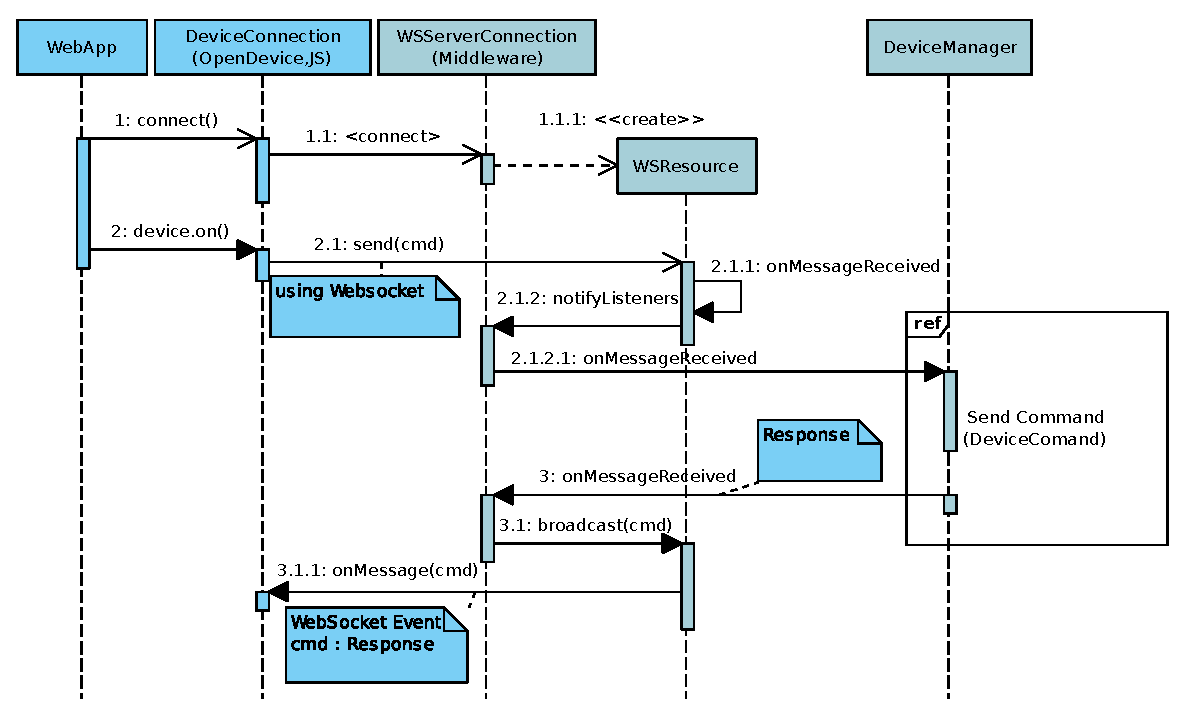
\includegraphics[width=1\linewidth]{Imagens/Cap_4/seq_send_ws}
\par\end{centering}
\caption{Envio de comandos\label{fig:seq_send_ws}}
\end{figure}


\section{Protocolo\label{subsec:Protocolo}}

Esta seção apresenta o protocolo do OpenDevice. As principais características
do protocolo é que ele foi projetado para ser um protocolo aberto,
leve, simples, de fácil implementação, legível para humanos e voltado
para dispositivos com restrições de memória e processamento, como
por exemplo, microcontroladores (AVR 8-bits, 2Kb de RAM).

O protocolo é baseado em ASCII (assim como o HTTP), orientado a mensagens/comandos
e assíncrono. Surgiu de algumas influências do protocolo MIDI (formato
usado para comunicação com instrumentos musicais) e do protocolo REST
na sua estrutura básica. 

O protocolo foi projetado para permitir a abstração, controle de dispositivos
(atuadores), realizar a leitura de sensores e ser de fácil extensão,
mas não limitado a isto. Ele pode ser utilizado em conjunto com outros
protocolos, como WebSocket e MQTT, e com outras tecnologias de comunicação,
como: USB, Bluetooth, Ethernet, Wi-Fi, etc. 


\subsection{Formato da Mensagem}

Os comandos do OpenDevice possuem um ``cabeçalho'' fixo, contento
o tipo do comando (\emph{CommandType}) e o ID do comando, em seguida,
o bloco \emph{``Command Extension}'', que varia de acordo com o
tipo de comando. 

\begin{figure}[H]
\begin{centering}
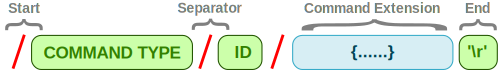
\includegraphics[width=0.8\linewidth]{Imagens/Cap_4/protocol_spec}
\par\end{centering}
\caption{Formato do protocolo OpenDevice \label{fig:protocol_spec}}
\end{figure}

\begin{itemize}
\item O \textbf{tipo do comando} define a estrutura do bloco ``\emph{Command
Extension}''. Os tipos suportados estão definidos na tabela \ref{tab:CommandType}. 
\item O \textbf{ID} do comando é numérico, sequencial e gerenciado pela
aplicação cliente. Ele serve para a aplicação identificar o retorno(resposta)
de algum comando enviado. Quando atinge seu valor máximo a contagem
reinicia.
\item Os blocos do comando são separados através do caractere ``/''.
\item O comando finaliza com o terminador ``\textbackslash{}r'' (Carriage
return).
\end{itemize}
\noun{Observação:} Na implementação atual do firmware, tanto o ``tipo
do comando'' quanto o ``id'', são armazenados em varáveis de 8bits
(uint8\_t / byte), limitando a valores na faixa de 0 a 255. Porém,
os mesmos são parametrizados podendo escolher outros tipos como: uint16\_t
ou uint32\_t.

\subsubsection{Convenções e pontos em aberto}

Algumas convenções foram adotadas para determinar observações, e destacar
pontos em aberto. Caso o texto apresente ``{[}{*}Numero{]}'', significa
que deve ser verificado as observações abaixo:
\begin{itemize}
\item Observação {[}{*}1{]}\noun{:} Na implementação atual do firmware,
o ``DeviceID'' é armazenado em uma variável de 8bits (byte), porém,
o tipo é parametrizável.
\item Observação {[}{*}2{]}\noun{: }Significa que o parâmetro ou tipo é
configurável. 
\item Observação {[}{*}3{]}\noun{:} Significa que a versão atual do firmware
não implementa o recurso.
\end{itemize}

\subsection{Tipos de Comandos}

A tabela \ref{tab:CommandType}, apresenta os tipos de comandos suportados.

\begin{table}[H]
\noindent\resizebox{\textwidth}{!}{
\begin{centering}
\begin{tabular}{|c|l|c|l|}
\hline 
Código & Tipo de Comando & Ref. & Formato\tabularnewline
\hline 
\hline 
1 & DIGITAL & \ref{subsec:DIGITAL} & {[}\#/\#{]}/\{DeviceID\}/\{value\}\tabularnewline
\hline 
2 & ANALOG & \ref{subsec:ANALOG} & {[}\#/\#{]}/\{DeviceID\}/\{value\}\tabularnewline
\hline 
3 & NUMERIC & \ref{subsec:NUMERIC} & {[}\#/\#{]}/\{DeviceID\}/\{value\}\tabularnewline
\hline 
4...9 & {[}Reservado{]} &  & –\tabularnewline
\hline 
10 & COMMAND\_RESPONSE & \ref{subsec:COMMAND_RESPONSE} & {[}\#/\#{]}/\{status\}/\{DeviceID?\}\tabularnewline
\hline 
11 & SET\_PROPERTY & \ref{subsec:SET_PROPERTY} & {[}\#/\#{]}/\{DeviceID\}/\{property\}/\{value\}\tabularnewline
\hline 
12 & GET\_PROPERTIES & \ref{subsec:GET_PROPERTIES} & {[}\#/\#{]}/\{DeviceID\}\tabularnewline
\hline 
13 & GET\_PROPERTIES\_RESPONSE & \ref{subsec:GET_PROPERTIES_RESPONSE} & {[}\#/\#{]}/\{DeviceID\}/{[}\{property1:value\},...,N{]}\tabularnewline
\hline 
14 & ACTION & \ref{subsec:ACTION} & {[}\#/\#{]}/\{DeviceID\}/\{action\}/{[}\{value1?\},...,\{valueN\}{]}\tabularnewline
\hline 
15 & GET\_ACTIONS & \ref{subsec:GET_ACTIONS} & {[}\#/\#{]}/\{DeviceID\}\tabularnewline
\hline 
16 & GET\_ACTIONS\_RESPONSE & \ref{subsec:GET_ACTIONS_RESPONSE} & {[}\#/\#{]}/\{DeviceID\}/{[}\{action1\},\{actionN\}{]}\tabularnewline
\hline 
16...19 & {[}Reservado{]} &  & –\tabularnewline
\hline 
20 & PING\_REQUEST & \ref{subsec:PING_REQUEST} & {[}\#/\#{]}{[}somente cabeçalho{]}\tabularnewline
\hline 
21 & PING\_RESPONSE & \ref{subsec:PING_RESPONSE} & {[}\#/\#{]}{[}somente cabeçalho{]}\tabularnewline
\hline 
22 & DISCOVERY\_REQUEST & \ref{subsec:DISCOVERY_REQUEST} & {[}\#/\#{]}{[}somente cabeçalho{]}\tabularnewline
\hline 
23 & DISCOVERY\_RESPONSE & \ref{subsec:DISCOVERY_RESPONSE} & {[}\#/\#{]}/\{name\}/\{port\}/\{deviceLength\}\tabularnewline
\hline 
24...29 & {[}Reservado{]} &  & –\tabularnewline
\hline 
30 & GET\_DEVICES & \ref{subsec:GET_DEVICES} & {[}\#/\#{]}/\{DeviceID?\}/\{value?\}\tabularnewline
\hline 
31 & GET\_DEVICES\_RESPONSE & \ref{subsec:GET_DEVICES_RESPONSE} & {[}\#/\#{]}/{[}\{DeviceInfo1\},\{DeviceInfoN?{]}\tabularnewline
\hline 
32 & DEVICE\_ADD & \ref{subsec:DEVICE_ADD} & {[}\#/\#{]}/\{DeviceInfo\}\tabularnewline
\hline 
33 & DEVICE\_DEL & \ref{subsec:DEVICE_DEL} & {[}\#/\#{]}/\{DeviceID?\}\tabularnewline
\hline 
41..100 & {[}Reservado{]} &  & \tabularnewline
\hline 
\end{tabular}
\par\end{centering}
}

\caption{Tipos de comandos do protocolo\label{tab:CommandType}}
\end{table}


\subsection{Comando: DIGITAL\label{subsec:DIGITAL}}

Este comando permite controlar os dispositivos digitais (atuadores)
ou notificar alguma mudança no estado/valor de um sensor. O comando
adiciona dois blocos adicionais: DeviceID e Value (Figura \ref{fig:protocol_cmd}). 

Ao enviar um comando para um dispositivo, por exemplo, ligar lâmpada,
o dispositivo deve retornar uma resposta (geralmente assíncrona),
com o status do comando. 

O formato da resposta é definida em \emph{``}\nameref{subsec:COMMAND_RESPONSE}'',
onde o ID da resposta será o mesmo ID do comando enviado.

\begin{figure}[H]
\begin{centering}
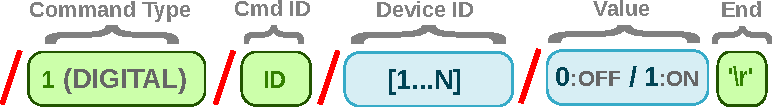
\includegraphics[width=0.8\linewidth]{Imagens/Cap_4/protocol_cmd_digital}
\par\end{centering}
\caption{Comando: DIGITAL\label{fig:protocol_cmd}}
\end{figure}

\begin{table}[H]
\begin{centering}
\begin{tabular}{|c|c|l|}
\hline 
Parâmetro & Tipo & Descrição\tabularnewline
\hline 
\hline 
DeviceID & byte {[}{*}1{]} & Identificador único que representa o dispositivo\tabularnewline
\hline 
Value & bool & 0 (Desligar / Desligado) ou 1 (Ligar / Ligado)\tabularnewline
\hline 
\end{tabular}
\par\end{centering}
\caption{Parâmetros - Comando: DIGITAL}
\end{table}


\subsection{Comando: ANALOG\label{subsec:ANALOG}}

Obedece o formado do ``\nameref{subsec:DIGITAL}'', mudando apenas
o tipo do comando, no caso 2, e o tipo de dado do bloco ``\emph{Value}'',
que pode aceitar valores do tipo \emph{``unsigned long}'', com tamanho
de 32 bits (4 bytes). 

Este comando pode ser utilizado tanto para sensores como para atuadores,
no caso de sensores, ele é utilizado para notificar um mudança de
estado (já que sensores são apenas para ``leitura'').

O formato da resposta é definida em \emph{``}\nameref{subsec:COMMAND_RESPONSE}'',
onde o ID da resposta será o mesmo ID do comando enviado.

\subsection{Comando: NUMERIC\label{subsec:NUMERIC}}

Obedece o formado do ``\nameref{subsec:ANALOG}''. Este comando
é utilizado em conjunto com os dispositivos (principalmente sensores)
do tipo \emph{NUMERIC}, que permitem o envio de informações repetidas.
Um exemplo, o sensor RFID, que gera um evento toda vez que uma etiqueta
é lida, mesmo sendo a mesma etiqueta.

\subsection{Reposta: COMMAND\_RESPONSE\label{subsec:COMMAND_RESPONSE}}

Representa a resposta de um determinado comando. As respostas são
associadas ao comando que a originou (requisição), através do atributo
``ID'' do cabeçalho fixo. Adicionalmente os comandos que referenciam
um dispositivo, na resposta, será incluído o mesmo ``DeviceID''
do comando da ``requisição''.

\begin{table}[H]
\begin{centering}
\begin{tabular}{|c|c|c|}
\hline 
\prth HEADER & \prtv Status & \prtv DeviceID\tabularnewline
\hline 
\end{tabular}
\par\end{centering}
\caption{Reposta: COMMAND\_RESPONSE}
\end{table}

\begin{table}[H]
\begin{centering}
\begin{tabular}{|c|c|l|}
\hline 
Parâmetro & Tipo & Descrição\tabularnewline
\hline 
\hline 
ID & byte {[}{*}2{]} & Mesmo ID enviado na requisição\tabularnewline
\hline 
Status & byte & Obedece aos valores da tabela: \ref{tab:CommandStatusResp}\tabularnewline
\hline 
DeviceID & byte {[}{*}1{]} (Opcional) & Mesmo ID enviado na requisição\tabularnewline
\hline 
\end{tabular}
\par\end{centering}
\caption{Parâmetros - Comando: COMMAND\_RESPONSE\label{tab:CommandStatusResp-1-1}}
\end{table}

\begin{table}[H]
\begin{centering}
\begin{tabular}{|c|c|}
\hline 
Status & Código\tabularnewline
\hline 
\hline 
SUCCESS & 200\tabularnewline
\hline 
NOT\_FOUND & 404\tabularnewline
\hline 
BAD\_REQUEST & 400\tabularnewline
\hline 
\textcolor{red}{UNAUTHORIZED {[}{*}3{]}} & 401\tabularnewline
\hline 
\textcolor{red}{FORBIDDEN {[}{*}3{]}} & 403\tabularnewline
\hline 
\textcolor{red}{PERMISSION\_DENIED {[}{*}3{]}} & 550\tabularnewline
\hline 
INTERNAL\_ERROR & 500\tabularnewline
\hline 
NOT\_IMPLEMENTED & 501\tabularnewline
\hline 
\end{tabular}
\par\end{centering}
\caption{Status da resposta do comando\label{tab:CommandStatusResp}}
\end{table}


\subsection{Comando: SET\_PROPERTY\label{subsec:SET_PROPERTY}}

Comando utilizado para atualizar alguma propriedade do dispositivo.
O formato da resposta é definido em \emph{``}\nameref{subsec:COMMAND_RESPONSE}''.

\begin{table}[H]
\begin{centering}
\begin{tabular}{|c|c|c|c|}
\hline 
\prth HEADER & \prtv DeviceID & \prtv property & \prtv value\tabularnewline
\hline 
\end{tabular}
\par\end{centering}
\caption{Comando: SET\_PROPERTY}
\end{table}

\begin{table}[H]
\begin{centering}
\begin{tabular}{|c|c|l|}
\hline 
Parâmetro & Tipo & Descrição\tabularnewline
\hline 
\hline 
DeviceID & byte {[}{*}1{]} & Identificador único que representa o dispositivo\tabularnewline
\hline 
property & String & Propriedade a ser alterada\tabularnewline
\hline 
value & String & Valor da propriedade\tabularnewline
\hline 
\end{tabular}
\par\end{centering}
\caption{Parâmetros: SET\_PROPERTY}
\end{table}


\subsection{Comando: GET\_PROPERTIES\label{subsec:GET_PROPERTIES}}

Comando utilizado para recuperar a lista de propriedades do dispositivo
e seus respectivos valores. O formato da resposta é definido em \emph{``}\nameref{subsec:GET_PROPERTIES_RESPONSE}''

\begin{table}[H]
\begin{centering}
\begin{tabular}{|c|c|}
\hline 
\prth HEADER & \prtv DeviceID\tabularnewline
\hline 
\end{tabular}
\par\end{centering}
\caption{Comando: GET\_PROPERTIES}
\end{table}

\begin{table}[H]
\begin{centering}
\begin{tabular}{|c|c|l|}
\hline 
Parâmetro & Tipo & Descrição\tabularnewline
\hline 
\hline 
DeviceID & byte {[}{*}1{]} & Identificador único que representa o dispositivo\tabularnewline
\hline 
\end{tabular}
\par\end{centering}
\caption{Parâmetros: GET\_PROPERTIES}
\end{table}


\subsection{Comando: GET\_PROPERTIES\_RESPONSE\label{subsec:GET_PROPERTIES_RESPONSE}}

Resposta do comando ``\emph{GET\_PROPERTIES}'', com a lista de propriedades
do dispositivo. A lista é retornada no formato de um Array, e os elementos
no formato: ``Propriedade:Valor''.

\begin{table}[H]
\begin{centering}
\begin{tabular}{|c|c|c|}
\hline 
\prth HEADER & \prtv DeviceID & \prtv{[}property:value,...,propertyN:value{]}\tabularnewline
\hline 
\end{tabular}
\par\end{centering}
\caption{Comando: GET\_PROPERTIES\_RESPONSE}
\end{table}

\begin{table}[H]
\begin{centering}
\begin{tabular}{|c|c|l|}
\hline 
Parâmetro & Tipo & Descrição\tabularnewline
\hline 
\hline 
DeviceID & byte {[}{*}1{]} & Identificador único que representa o dispositivo\tabularnewline
\hline 
property & String & Propriedade\tabularnewline
\hline 
value & String & Valor da propriedade\tabularnewline
\hline 
\end{tabular}
\par\end{centering}
\caption{Parâmetros: GET\_PROPERTIES\_RESPONSE}
\end{table}


\subsection{Comando: ACTION\label{subsec:ACTION}}

Comando usado para executar as ações definidas pelos dispositivos.
As ações podem receber uma lista de valores, que são especificados
em formato de Array. O formato da resposta é definido em \emph{``}\nameref{subsec:COMMAND_RESPONSE}''.

\begin{table}[H]
\begin{centering}
\begin{tabular}{|c|c|c|c|}
\hline 
\prth HEADER & \prtv DeviceID & \prtv action & \prtv{[}\{value1\},...,\{valueN\}{]}\tabularnewline
\hline 
\end{tabular}
\par\end{centering}
\caption{Comando: ACTION}
\end{table}

\begin{table}[H]
\begin{centering}
\begin{tabular}{|c|c|l|}
\hline 
Parâmetro & Tipo & Descrição\tabularnewline
\hline 
\hline 
DeviceID & byte {[}{*}1{]} & Identificador único que representa o dispositivo\tabularnewline
\hline 
action & String & Ação que deve ser executada\tabularnewline
\hline 
value & Array{[}String{]} (Opcional) & A lista de valores que a ação recebe\tabularnewline
\hline 
\end{tabular}
\par\end{centering}
\caption{Parâmetros: ACTION}
\end{table}


\subsection{Comando: GET\_ACTIONS\label{subsec:GET_ACTIONS}}

Comando utilizado para recuperar a lista de ações definidas para o
dispositivo. O formato da resposta é definido em \emph{``}\nameref{subsec:GET_ACTIONS_RESPONSE}''

\begin{table}[H]
\begin{centering}
\begin{tabular}{|c|c|}
\hline 
\prth HEADER & \prtv DeviceID\tabularnewline
\hline 
\end{tabular}
\par\end{centering}
\caption{Comando: GET\_ACTIONS}
\end{table}

\begin{table}[H]
\begin{centering}
\begin{tabular}{|c|c|l|}
\hline 
Parâmetro & Tipo & Descrição\tabularnewline
\hline 
\hline 
DeviceID & byte {[}{*}1{]} & Identificador único que representa o dispositivo\tabularnewline
\hline 
\end{tabular}
\par\end{centering}
\caption{Parâmetros: GET\_ACTIONS}
\end{table}


\subsection{Comando: GET\_ACTIONS\_RESPONSE\label{subsec:GET_ACTIONS_RESPONSE}}

Resposta do comando ``\emph{GET\_ACTIONS}'', com a lista de ações
do dispositivo. A lista é retornada no formato de um Array.

\begin{table}[H]
\begin{centering}
\begin{tabular}{|c|c|c|}
\hline 
\prth HEADER & \prtv DeviceID & \prtv {[}\{action1\},..,\{actionN\}{]}\tabularnewline
\hline 
\end{tabular}
\par\end{centering}
\caption{Comando: GET\_ACTIONS\_RESPONSE}
\end{table}

\begin{table}[H]
\begin{centering}
\begin{tabular}{|c|c|l|}
\hline 
Parâmetro & Tipo & Descrição\tabularnewline
\hline 
\hline 
DeviceID & byte {[}{*}1{]} & Identificador único que representa o dispositivo\tabularnewline
\hline 
action & Array{[}String{]} & Lista de ações do dispositivo\tabularnewline
\hline 
\end{tabular}
\par\end{centering}
\caption{Parâmetros: GET\_ACTIONS\_RESPONSE}
\end{table}


\subsection{Comando: PING\_REQUEST\label{subsec:PING_REQUEST}}

Comando enviado pelo firmware para notificar que está em funcionamento
e ao mesmo tempo monitora o status do middleware/aplicação. 

Este comando não possui parâmetros adicionais, apenas cabeçalho. O
formato da resposta é definido em \emph{``}\nameref{subsec:PING_RESPONSE}''

\subsection{Resposta: PING\_RESPONSE\label{subsec:PING_RESPONSE}}

Resposta para o comando ``PING\_REQUEST''. Este comando não possui
parâmetros adicionais, apenas cabeçalho.

\subsection{Comando: DISCOVERY\_REQUEST\label{subsec:DISCOVERY_REQUEST}}

Comando utilizado para realizar a descoberta de dispositivos (módulos)
em uma rede. Geralmente é enviado via \emph{broadcast}. Este comando
não possui parâmetros adicionais, apenas cabeçalho.

\subsection{Resposta: DISCOVERY\_RESPONSE\label{subsec:DISCOVERY_RESPONSE}}

Resposta com as informações de descoberta dos dispositivos (módulos)
. 

\begin{table}[H]
\begin{centering}
\begin{tabular}{|c|c|c|c|c|}
\hline 
\prth HEADER & \prtv name & \prtv type & \prtv deviceLength & \prtv port\tabularnewline
\hline 
\end{tabular}
\par\end{centering}
\caption{Comando: GET\_ACTIONS\_RESPONSE}
\end{table}

\begin{table}[H]
\begin{centering}
\begin{tabular}{|c|c|l|}
\hline 
Parâmetro & Tipo & Descrição\tabularnewline
\hline 
\hline 
name & String & Nome do dispositivo (módulo)\tabularnewline
\hline 
type & int & Identifica o tipo de dispositivo (NODE/MANAGER)\tabularnewline
\hline 
deviceLength & int & Quantidades de dispositivos que o módulo possui\tabularnewline
\hline 
port & int (Opcional) & Porta de conexão (apenas para TCP/WIFI)\tabularnewline
\hline 
\end{tabular}
\par\end{centering}
\caption{Parâmetros: DISCOVERY\_RESPONSE}
\end{table}


\subsection{Comando: GET\_DEVICES\label{subsec:GET_DEVICES}}

Comando usado para obter informações de um ou mais dispositivos. Os
campos 'DeviceID' e 'Valor' são opcionais e podem ser usados como
filtro para o comando. 

\begin{table}[H]
\begin{centering}
\begin{tabular}{|c|c|c|}
\hline 
\prth HEADER & \prtv DeviceID & \prtv Value\tabularnewline
\hline 
\end{tabular}
\par\end{centering}
\caption{Comando: GET\_DEVICES}
\end{table}

\begin{table}[H]
\begin{centering}
\begin{tabular}{|c|c|l|}
\hline 
Parâmetro & Tipo & Descrição\tabularnewline
\hline 
\hline 
DeviceID (Opcional) & byte {[}{*}1{]} & Informar o ID do dispositivo ou 0 para todos\tabularnewline
\hline 
Value (Opcional) & \emph{unsigned long} & Permite filtrar por valor ou 0 para todos\tabularnewline
\hline 
\end{tabular}
\par\end{centering}
\caption{Parâmetros: GET\_DEVICES}
\end{table}


\subsection{Resposta: GET\_DEVICES\_RESPONSE\label{subsec:GET_DEVICES_RESPONSE}}

Resposta do comando ``GET\_DEVICES'', com a lista de dispositivos
cadastrados. O bloco ``\emph{Command Extension}'', consiste em um
Array de objetos do ``\nameref{subsec:Objeto_DeviceInfo}'', separados
por ``,''. A quantidade de dispositivos deve ser inferida automaticamente.

\begin{table}[H]
\begin{centering}
\begin{tabular}{|c|c|}
\hline 
\prth HEADER & \prtv {[}DeviceInfo,...,DeviceInfoN{]}\tabularnewline
\hline 
\end{tabular}
\par\end{centering}
\caption{Resposta: GET\_DEVICES\_RESPONSE}
\end{table}

\begin{table}[H]
\begin{centering}
\begin{tabular}{|c|c|c|}
\hline 
Parâmetro & Tipo & Descrição\tabularnewline
\hline 
\hline 
ID & byte {[}{*}2{]} & Mesmo ID enviado da requisição\tabularnewline
\hline 
DeviceInfo & Array{[}DeviceInfo{]} & Lista dos atributos do \nameref{subsec:Objeto_DeviceInfo}\tabularnewline
\hline 
\end{tabular}
\par\end{centering}
\caption{Parâmetros - Resposta: GET\_DEVICES\_RESPONSE}
\end{table}


\subsection{Comando: DEVICE\_ADD\label{subsec:DEVICE_ADD}}

Comando utilizado para configurar dinâmicamente os dispositivos de
um módulo. O formato da resposta é definido em \emph{``}\nameref{subsec:COMMAND_RESPONSE}''.

\begin{table}[H]
\begin{centering}
\begin{tabular}{|c|c|}
\hline 
\prth HEADER & \prtv DeviceInfo\tabularnewline
\hline 
\end{tabular}
\par\end{centering}
\caption{Comando: DEVICE\_ADD}
\end{table}

\begin{table}[H]
\begin{centering}
\begin{tabular}{|c|c|l|}
\hline 
Parâmetro & Tipo & Descrição\tabularnewline
\hline 
\hline 
DeviceInfo & DeviceInfo & Lista dos atributos do \nameref{subsec:Objeto_DeviceInfo}\tabularnewline
\hline 
\end{tabular}
\par\end{centering}
\caption{Parâmetros: DEVICE\_ADD}
\end{table}


\subsection{Comando: DEVICE\_DEL\label{subsec:DEVICE_DEL}}

Comando utilizado deletar o(s) dispositiv(o) de um módulo. O formato
da resposta é definido em \emph{``}\nameref{subsec:GET_ACTIONS_RESPONSE}''

\begin{table}[H]
\begin{centering}
\begin{tabular}{|c|c|}
\hline 
\prth HEADER & \prtv DeviceID\tabularnewline
\hline 
\end{tabular}
\par\end{centering}
\caption{Comando: DEVICE\_DEL}
\end{table}

\begin{table}[H]
\begin{centering}
\begin{tabular}{|c|c|l|}
\hline 
Parâmetro & Tipo & Descrição\tabularnewline
\hline 
\hline 
DeviceID & byte {[}{*}1{]} (Opcioanl) & Informar o ID do dispositivo ou 0 para todos\tabularnewline
\hline 
\end{tabular}
\par\end{centering}
\caption{Parâmetros: DEVICE\_DEL}
\end{table}


\subsection{Tipo: DeviceInfo\label{subsec:Objeto_DeviceInfo}}

Representa as informações e um dispositivo. É representado como um
Array no seguinte formato: \inputencoding{latin9}\lstinline![ID, PIN, VALUE, TARGET, SENSOR, TYPE]!\inputencoding{utf8}.

\begin{table}[H]
\begin{centering}
\begin{tabular}{|c|c|l|}
\hline 
Atributo & Tipo & Descrição\tabularnewline
\hline 
\hline 
ID & byte {[}{*}2{]} & ID do dispositivo \tabularnewline
\hline 
PIN & byte & Pino que o dispositivo está vinculado\tabularnewline
\hline 
VALUE & unsigned long & Valor atual do dispositivo\tabularnewline
\hline 
TARGET & byte & Quando for sensor, representa outro dispositivo (Opcional)\tabularnewline
\hline 
SENSOR & bool & 0 para atuador, 1 para sensor\tabularnewline
\hline 
TYPE & byte & Tipo de dispositivo (Tabela \ref{tab:TipoDispositivo})\tabularnewline
\hline 
\end{tabular}
\par\end{centering}
\caption{Objeto: DeviceInfo}
\end{table}

\begin{table}[H]
\begin{centering}
\begin{tabular}{|c|c|}
\hline 
Código & Tipo\tabularnewline
\hline 
\hline 
1 & DIGITAL\tabularnewline
\hline 
2 & ANALOG\tabularnewline
\hline 
3 & NUMERIC\tabularnewline
\hline 
\end{tabular}
\par\end{centering}
\caption{Tipos de Dispositivos\label{tab:TipoDispositivo}}
\end{table}







\chapter{Avaliação Experimental\label{sec:Avaliacao-Experimental}}

Este capítulo apresenta avaliação experimental da implementação da
arquitetura apresentada no capítulo \ref{sec:Arquitetura}. Os objetivos
gerais desta avaliação e a estruturação da mesma são apresentados
a seguir.

Na seção \ref{par:Hardwares-Testados}, foram realizados testes em
diferentes hardwares, permitindo avaliar sua capacidade de adaptabilidade
e compatibilidade tanto da perspectiva do middleware, quanto do firmware.
Na seção \ref{sec:Testes-de-Performance}, foram conduzidos testes
de performance com diferentes tecnologias de comunicação e protocolos,
permitindo avalizar a capacidade da arquitetura de lidar com tecnologias
heterogêneas e avaliar o desempenho e latências de comunicação. A
seção \ref{sec:Integracao3D}, apresenta experimentos de integração
com ambientes de desenvolvimento de jogos 3D (\emph{Game Engines}),
\emph{Blender} e \emph{jMonkeyEngine.} Estas ferramentas podem ser
utilizadas para criar ambientes de simulação, facilitando a criação
de aplicações de IoT, sem depender de um ambiente ou hardware real.
Por fim, a seção \ref{sec:Estudo-de-Caso}, apresenta um estudo de
caso, que permite avaliar a arquitetura proposta em um contexto real.
O contexto apresentado, está relacionado à automação residencial,
focando, principalmente, no controle de acesso usando a tecnologia
RFID.

\section{Hardwares Testados\label{par:Hardwares-Testados}}

Os testes realizados com os hardware estão subdivididos nas categorias
de microcontroladores (onde é executado o firmware) e os hardwares
na categoria de mini PCs que possuem um poder de processamento maior
e são destinados a executar o middleware ou aplicação construída utilizando
o framework.

\subsection{Microcontroladores (Firmware)}

Apesar do firmware ser construído com base na API do Arduino, o que
o tornaria automaticamente compatível com uma série de dispositivos
\cite{arduino-comp1,arduino-comp2,arduino-comp3}, os testes demostraram
que alguns microcontroladores possuem peculiaridades que têm que ser
levadas em consideração, principalmente pelo nível de abstração que
é proposto pelo sistema de configuração dinâmico de conexões que é
implementado (seção \ref{subsec:ConfiguracaoDinamica}). Como exemplo,
o firmware deve ser capaz de identificar quando estiver rodando em
um ESP8266, e realizar as configurações para conexão Wi-Fi sem necessidade
de modificações na aplicação/firmware.

A tabela \ref{tab:HardwaresTestados1} apresenta a lista de hardwares
dessa categoria que foram testados. Em seguida é apresentada a tabela
\ref{tab:HardwaresTestados1-mod}, com os módulos de conexão testados.

\begin{table}[h]
\begin{centering}
\begin{tabular}{|c|c|c|}
\hline 
Nome & Processador & Arquitetura\tabularnewline
\hline 
\hline 
Arduino UNO & ATmega328P - 16 MHz & AVR 8-bit\tabularnewline
\hline 
Arduino Nano & ATmega328P - 16 MHz & AVR 8-bit\tabularnewline
\hline 
Arduino Leonardo & ATmega32u4 - 16 MHz & AVR 8-bit\tabularnewline
\hline 
\textcolor{black}{Arduino MEGA} & ATmega2560 - 16 MHz & AVR 8-bit\tabularnewline
\hline 
Arduino Yun & ATmega32U4 / AR9331 Linux & AVR 8-bit\tabularnewline
\hline 
\textcolor{black}{Arduino Due} & ATSAM3X8E - 84 MHz & ARM 32-bit \tabularnewline
\hline 
ESP8266 & SoC (Tensilica's L106) - 80 MHz & RISC 32-bit\tabularnewline
\hline 
Stellaris Launchpad & LM4F120H5QR - 80 MHz & ARM M4F 32-bit \tabularnewline
\hline 
Digispark & ATtiny85 - 20MHz & AVR 8-bit\tabularnewline
\hline 
Teensy 3.1 & MK20DX256 - 72 MHz & ARM M4 32-bit\tabularnewline
\hline 
\end{tabular}
\par\end{centering}
\caption{Hardwares Testados (Microcontroladores)\label{tab:HardwaresTestados1}}
\end{table}

\begin{table}[h]
\begin{centering}
\begin{tabular}{|c|c|}
\hline 
Módulo & Conexão\tabularnewline
\hline 
\hline 
Arduino Ethernet Shield & Ethernet\tabularnewline
\hline 
Módulo ENC28J60 & Ethernet\tabularnewline
\hline 
ESP8266 (AT Mode) & Wi-Fi\tabularnewline
\hline 
HC-05 / HC-06 & Bluetooth SPP\tabularnewline
\hline 
\end{tabular}
\par\end{centering}
\caption{Hardwares Testados (Módulos)\label{tab:HardwaresTestados1-mod}}
\end{table}


\subsection{Mini PCs}

No trabalho, nomeamos de mini PCs, os hardware capazes de executar
um sistema operacional completo, como o Linux, e que possuem 512MB
de memória RAM ou superior. Hardwares baseados na arquitetura ARM
são elegíveis para suporte a máquina virtual Java (JVM), consequentemente
tendo suporte para execução do middleware. Entretanto a forma de acesso
aos periféricos dos mesmos, como os pinos de GPIO, são específicos
de cada plataforma. Não existe uma especificação genérica como a disponível
no framework do Arduino, que abstraia o acesso aos pinos de GPIO de
uma forma unificado. Uma proposta é API \emph{Device I/O}\cite{device-io:wiki},
porém, é um especificação nova e sua compatibilidade é limitada. 

\begin{table}[h]
\begin{centering}
\begin{tabular}{|c|c|c|}
\hline 
Nome & Arquitetura & RAM \tabularnewline
\hline 
\hline 
Raspberry Pi Model B (Alpha) & ARM & 256MB\tabularnewline
\hline 
BeagleBone Black & ARM & 512MB\tabularnewline
\hline 
\end{tabular}
\par\end{centering}
\caption{Hardwares Testados (Mini PCs)\label{tab:HardwaresTestados2}}
\end{table}


\section{Testes de Performance\label{sec:Testes-de-Performance}}

O objetivo deste experimento é avaliar a performance do middleware,
implementações das tecnologias de comunicação e do firmware.

\subsection{Procedimento de Medição}

Os experimentos foram executados através da ferramenta JMH\footnote{http://openjdk.java.net/projects/code-tools/jmh/},
que permite a criação de \emph{micro-benchmarks} em Java, isolando
alguns comportamentos da JVM, aproximando ao máximo de um ambiente
real. 

Os seguintes parâmetros de configuração foram utilizados na execução
dos testes:
\begin{itemize}
\item Iterações de pré-execução: 2;
\item Tempo de execução das iterações de pré-execução: 2s;
\item Iterações de coleta de dados: 20;
\item Tempo de cada iteração: 1s;
\item Argumentos da JVM: ``-server''.
\end{itemize}
As iterações de ``pré-execução'' são utilizadas para garantir que
a JVM, todas as classes da aplicação e bibliotecas, sejam carregadas
completamente, evitando interferência de acesso ao disco. 

Em cada iteração de coletas de dados são enviados um série de comandos
(\emph{DeviceCommand}) para os dispositivos, durante o período definido
(1s). Em cada iteração, são enviados o máximo de comandos possíveis
de forma sequencial e síncrona, permitindo calcular o tempo médio
de resposta de cada comando.

Ao final de todas iterações definidas (20), as estatísticas são geradas
pela ferramenta.

\subsection{Métrica Utilizada}

A métrica utilizada é o tempo de resposta fim-a-fim. Após todas iterações
serem executadas, é calculado o tempo médio de resposta de cada iteração
e em seguida, o tempo médio de reposta geral de todas iterações e
o erro médio.

O tempo de resposta, inclui o tempo para geração da mensagem no middleware,
transmissão, processamento e execução da ação no dispositivo e recebimento
da resposta.

\subsection{Resultados: Conexão USB}

\begin{figure}[H]
\begin{centering}
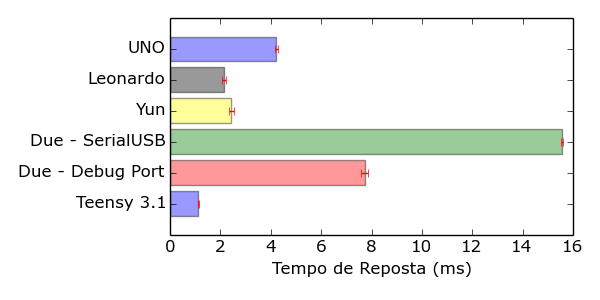
\includegraphics[width=0.8\linewidth]{Imagens/Cap_5/usb}
\par\end{centering}
\caption{Teste de performance - USB\label{fig:perf-usb}}
\end{figure}


\subsection{Resultados: Conexão Bluetooth}

\begin{figure}[H]
\begin{centering}
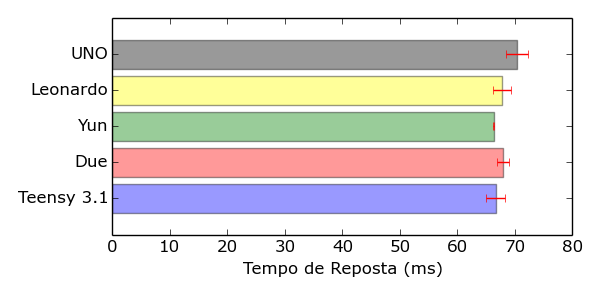
\includegraphics[width=0.8\linewidth]{Imagens/Cap_5/bluetooth}
\par\end{centering}
\caption{Teste de performance - Bluetooth\label{fig:perf-bluetooth}}
\end{figure}


\subsection{Resultados: Conexão Ethernet}

\begin{figure}[H]
\begin{centering}
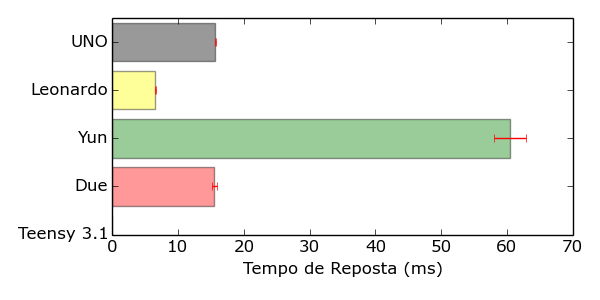
\includegraphics[width=0.8\linewidth]{Imagens/Cap_5/ethernet}
\par\end{centering}
\caption{Teste de performance - Ethernet\label{fig:perf-ethernet}}
\end{figure}


\section{Integração com Ambientes 3D\label{sec:Integracao3D}}

O desenvolvimento de aplicações para Internet das Coisas conta com
o desafio de ter que lidar com vários dispositivos físicos. Como alternativa
ambientes de simulação podem ser utilizados para executar os testes
e experimentos, antes de testar com os dispositivos reais. Outra possibilidade
para utilização dos ambientes 3D, é permitir a integração entre um
ambiente real e virtual.

Foram realizados testes de integração do OpenDevice com sistema de
desenvolvimento de jogos (\emph{Game Engine}), afim de validar uma
possível utilização dos mesmos para criação de ambientes de simulação.
Os experimentos realizados são detalhados a seguir.

\subsection{Integração - jMonkeyEngine.}

A \emph{jMonkeyEngine}\footnote{\emph{http://jmonkeyengine.org/}}
é uma ferramenta gratuita de código fonte aberto, utilizada para construção
de jogos 3D em Java. Possui uma boa documentação e ambiente de desenvolvimento
integrado. Devido sua implementação ser baseada na linguagem Java,
a integração com o OpenDevice se torna bastante simples e permite
a construção de uma aplicação de simulação que utiliza as APIs e módulos
do OpenDevice diretamente, sem a necessidade do middleware. 

No teste realizado, foi construída uma aplicação simples para validar
a integração, que consiste no mapeamento dos dispositivos físicos,
no caso 3 LEDs, e sua vinculação com objetos virtuais 3D da \emph{Game
Engine}. Ao clicar em algum objeto 3D, como os representados na figura
\ref{fig:jmonkey}, o OpenDevice localiza o dispositivo vinculado
e envia o comando para o acionamento do dispositivo físico.

\begin{figure}
\begin{centering}
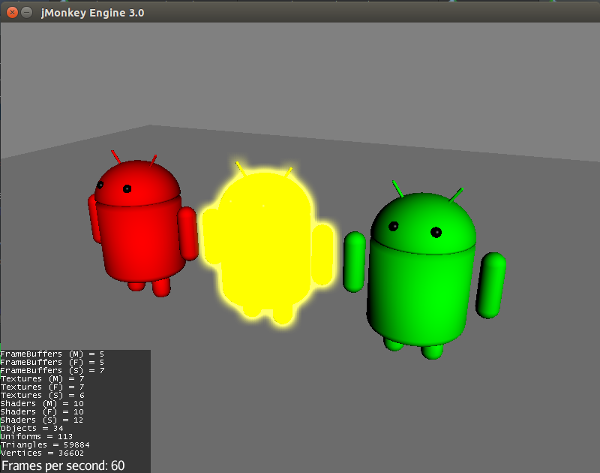
\includegraphics[width=0.8\linewidth]{Imagens/Cap_4/JMonkeyEngine}
\par\end{centering}
\caption{Integração com a JMonkeyEngine\label{fig:jmonkey}}
\end{figure}


\subsection{Integração - Blender.}

O \emph{Blender}\footnote{\emph{https://www.blender.org/}} é uma
ferramenta livre e de código fonte aberto, escrita em sua maior parte
utilizando a linguagem de programação Python. Ela possui ferramentas
para modelagem, animação, renderização e desenvolvimento de Jogos.
O diferencial em relação à \emph{jMonkeyEngine,} é que o \emph{Blender}
possui uma série de facilidades para configurações de eventos e vinculações
de scripts em Python utilizando apenas a interface gráfica.

Para permitir a integração com o OpenDevice, foi necessária a criação
de uma biblioteca cliente em Python, que implementa o protocolo do
OpenDevice e permite uma comunicação bidirecional através de uma comunicação
TCP. O experimento realizado (Figura \ref{fig:blender1}), é similar
ao experimento realizado com a \emph{jMonkeyEngine}, permitindo fazer
a vinculação entre objetos virtuais 3D e os dispositivos físicos\footnote{Vídeo do experimento da figura \ref{fig:blender1}: http://youtu.be/b3PbOPIMHmY}.

Para validar a performance da integração, foram realizados testes
visuais do tempo de resposta entre duas aplicações gráficas (Figura
\ref{fig:blender2}), uma escrita em Java (executando o middleware)
e outra Python. Verificou-se que as duas interfaces respondem em tempo
real às modificações na barra de rolagem (slider) em ambas interfaces\footnote{Vídeo do experimento da figura \ref{fig:blender2}: http://youtu.be/j4dMnAPZu70}.

\begin{figure}[h]
\begin{centering}
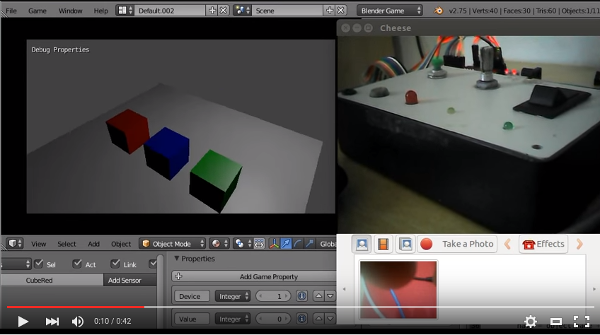
\includegraphics[width=1\linewidth]{Imagens/Cap_4/Blender}
\par\end{centering}
\caption{Integração com o Blender\label{fig:blender1}}
\end{figure}

\begin{figure}[h]
\begin{centering}
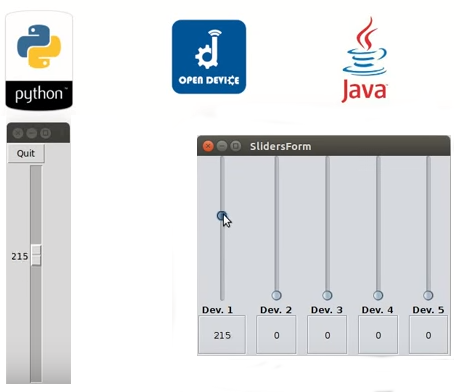
\includegraphics[width=0.7\linewidth]{/media/ricardo/Dados/Dropbox/Mestrado/Dissertacao/Imagens/Cap_4/Blender2}
\par\end{centering}
\caption{Teste de desempenho do cliente Python\label{fig:blender2}}
\end{figure}


\section{Estudo de Caso\label{sec:Estudo-de-Caso}}

A arquitetura descrita conforme a seção \ref{sec:Arquitetura}, foi
implementada vários testes foram conduzidos para validar os componentes
da arquitetura em relação ao design, integração e performance. Nesta
seção, faremos um estudo de caso baseado em um cenário real, permitindo
avaliar a integração entre os componentes da arquitetura e as capacidades
de evolução do framework proposto.

\subsection{Resumo}

O cenário escolhido para validação da proposta consiste em um sistema
de controle de acesso, usando a tecnologia RFID e alguns elementos
de automação residencial. A estratégia utilizada consiste na elaboração
de um cenário mais simples e sua posterior evolução para um cenário
mais complexo, integrando outros dispositivos e plataformas: Hardware,
Desktop, Web/Cloud e Mobile. O projeto será implantado nas instalações
do prédio denominado ``GEDAI'', onde está instalada a CriativaSoft
(empresa do autor) e outras duas empresas, sendo utilizado para o
controle de acesso dos funcionários. 

Os principais objetivos são: (1) avaliar os componentes da arquitetura
em conjunto, (2) validar os modelos de comunicação Cloud e Local,
(3) avaliar a integração com novos dispositivos (sensores e atuadores),
(4) avaliar a integração com dispositivos IP que utilizam outros protocolos,
(5) avaliar a integração com aplicações cliente Mobile(Android) e
(5) avaliar as capacidades de extensibilidade da plataforma.

\subsection{Ambiente de Teste}

Neste experimento serão utilizados hardwares de baixo custo, como
o Arduino, ESP8266 e Raspberry Pi, os demais sensores e atuadores
utilizados serão descritos nas seções seguintes. O middleware foi
implantado em um servidor na Amazon EC2, permitindo que aplicações
cliente controlem e recebam informações dos dispositivos pela Internet.

O experimento será avaliado em dois cenários, descritos e detalhados
a seguir.


\subsection{Cenário 1}

Este cenário tem como objetivo avalizar a utilização da arquitetura
do OpenDevice para criação de projetos simples para Internet das Coisas,
utilizando componente e hardwares existentes no mercado para criação
de projetos inovadores. Como mencionado, este cenário consiste na
criação de uma aplicação para controle de acesso usando RFID, conforme
apresentado na figura \ref{fig:cenario1}. Neste cenário, o hardware
está conectada à Internet através de uma comunicação Ethernet ou Wi-Fi
e se comunica com o middleware utilizando o protocolo do OpenDevice
em conjunto com o protocolo MQTT. Este cenário tem como característica
ser um cenário de fácil implantação. 

Para implementação dessa aplicação, foi utilizado o Arduino Yún, uma
versão do Arduino que possui conexão Ethernet e Wi-Fi já embutidas
na própria placa, e executa uma versão customizada no Linux para roteadores,
o OpenWrt-Yún\cite{openwrt-yun}, porém é possível utilizar qualquer
outra versão do Arduino, com um módulo que forneça uma comunicação
IP. A leitura dos cartões de acesso é feita por um leitor RFID de
proximidade que trabalha na frequência 13.56 MHz. O leitor é baseado
no processador MFRC522\cite{MFRC522} da empresa NXP, compatível com
cartões/tags RFID padrão ISO 14443A. A comunicação com este leitor
é realizada através do protocolo SPI\cite{spi1,spi2}.

\begin{figure}[H]
\begin{centering}
\includegraphics[width=1\linewidth]{Imagens/Cap_5/diagrama_caso1}
\par\end{centering}
\caption{Diagrama - Cenário 1 \label{fig:cenario1}}
\end{figure}


\subsubsection*{Estruturação do projeto:}

Neste cenário foram implementados duas aplicações: (1) uma aplicação
embarcada~(firmware), que faz o gerenciamento dos dispositivos físicos,
e (2) uma aplicação Java que utiliza o framework do OpenDevice, que
é a responsável pela validação dos cartões lidos. O firmware, utiliza
as bibliotecas do OpenDevice, MQTT\cite{lib-mqtt} e do leitor RFID
(MFRC522)\cite{lib-MFRC522}. A aplicação Java, é uma aplicação bem
simples, utilizando o módulo de servidor MQTT embarcado, o módulo
core da plataforma e um banco de dados em memória chamado MapDB\cite{mapdb},
com suporte a serialização em disco. O MapDB foi escolhido por ser
o mesmo utilizado na implementação do servidor MQTT (baseado no Moquette).

\subsubsection*{Descrição básica de funcionamento}

Ao detectar a presença de alguma etiqueta/cartão RFID, o firmware
envia a notificação para aplicação Java, que verifica a existência
do código lido no cache em memória (aumentando a performance) e envia
a resposta de confirmação de volta para o firmware, através de um
comando customizado (action), chamado \emph{``onAuthFinish}''. 

Na função ``\emph{onAuthFinish}'', definida pelo firmware, ele verifica
o parâmetro enviado pela aplicação, se a autenticação foi realizada,
em caso positivo, é emitido um sinal sonoro e liberado a fechadura
elétrica. Em caso negativo, é emitido um sinal sonoro longo e o acionamento
de um LED vermelho, permitindo o usuário identificar a não autorização.

O firmware conta com uma função que emite um alerta (sonoro e visual),
caso o servidor (aplicação Java) não efetue a resposta até um tempo
limite. É possível, também, a definição de chaves mestre, que não
necessitam de autenticação ``on-line'', permitindo a a liberação
do acesso caso não exista conectividade com a Internet.


\subsection{Cenário 2}

O cenário 2, representado pela figura \ref{fig:cenario2}, pode ser
considerado uma complementação do cenário 1, focado no controle de
acesso, mas incluindo novos elementos de automação. Neste cenário
é utilizado um servidor local, executando em um Raspberry Pi (ou BeagleBone),
e o mesmo está sincronizado com o middleware na Internet. 

O objetivo é avaliar o gerenciamento de vários dispositivos, a integração
com uma câmera IP (que opera com protocolo próprio), a interface entre
uma aplicação Mobile e dispositivos físicos pela Internet e a integração
entre uma aplicação local e o middleware instalado em um servidor
na nuvem.

Além do controle de acesso, usando RFID, este cenário integra uma
campainha sem fio, operando na frequência 433Mhz, uma câmera IP (clone
da Foscam) e um emissor de infra-vermelho para controle do ar-condicionado
da sala de reunião. 

\begin{figure}[H]
\begin{centering}
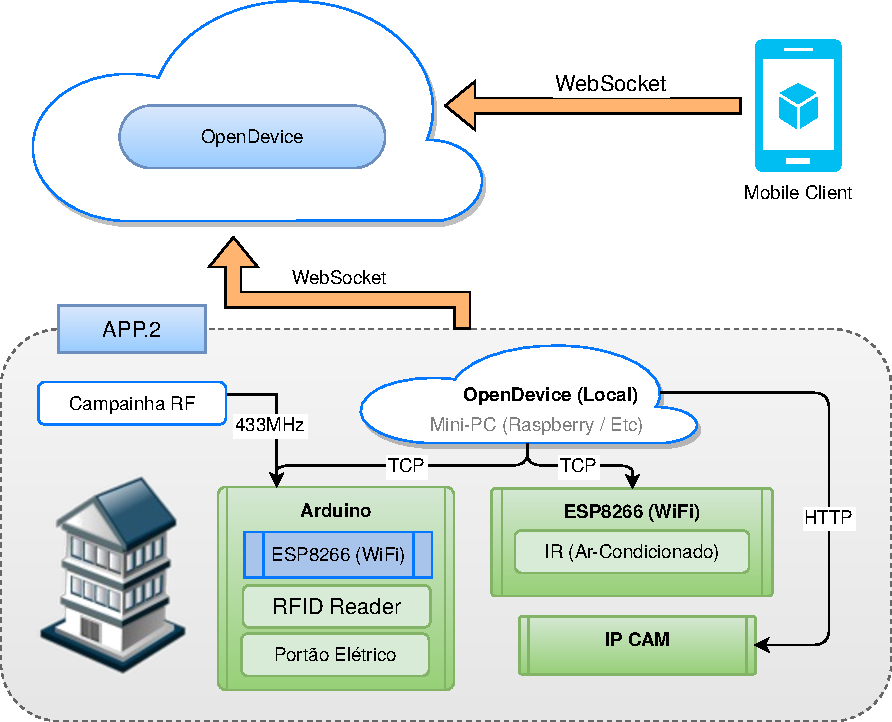
\includegraphics[width=1\linewidth]{Imagens/Cap_5/diagrama_caso2}
\par\end{centering}
\caption{Diagrama - Cenário 2 \label{fig:cenario2}}
\end{figure}


\subsubsection*{Descrição básica de funcionamento}

Quando a campainha é pressionada, o receptor RF 433Mhz acoplado ao
Arduino detecta o sinal e o firmware envia a notificação, via conexão
Wi-Fi, para a aplicação (ou middleware), que está executando no servidor
local. Em seguida, a aplicação captura a imagem da câmera IP e envia
uma notificação para as aplicações mobile, informando que uma visita
está aguardando a liberação, que pode ser realizada pelo próprio aplicativo
Mobile. 

\subsubsection*{Estruturação do projeto:}

Este cenário é composto por 5 aplicações/componentes, que serão detalhados
a seguir:
\begin{itemize}
\item \textbf{Dispositivo 1 (Arduino)}: Similar à implementação do cenário
1, com algumas modificações no hardware. Foi utilizado o Arduino UNO
e a conectividade Wi-Fi é fornecida pelo módulo ESP8266, utilizando
o firmware AT, conectado na porta UART do Arduino. Também foi incluído
um módulo receptor RF 433 Mhz que recebe o sinal da campainha. 
\item \textbf{Dispositivo 2 (ESP8266)}: O dispositivo que faz o controle
do ar-condicionado. Opera no modo independente (standalone), ou seja,
sem depender de outro componente. É programado com um firmware baseado
no framework do Arduino\cite{esp8266:arduino}, utilizando a biblioteca
do OpenDevice e a biblioteca para operar o emissor de infra-vermelho\footnote{https://github.com/markszabo/IRremoteESP8266}.
A comunicação com a aplicação local, é feita usando o protocolo MQTT
em conjunto com o protocolo do OpenDevice.
\item \textbf{Middleware Local}: Aplicação que executa localmente no Raspberry
Pi e responsável pelo gerenciamento de todos os dispositivos do projeto.
É baseada na versão padrão do middleware, e as regras específicas
para o projeto são implementadas através de extensões. As extensões
incluídas neste cenário adicionaram novas entidades persistentes,
novas interfaces Rest, suporte a novos dispositivos (câmera IP) e
novas páginas na interface administrativa do middleware. O sistema
de armazenamento utiliza a implementação padrão, baseada no Neo4J,
com suporte a JPA (Java Persistence API). A aplicação local possui
uma conexão com a versão do middleware que está implantado em um servidor
na nuvem (Amazon), permitindo que aplicações clientes controlem os
dispositivos pela Internet. 
\item \textbf{Middleware}: Implementação padrão disponibilizada pelo OpenDevice,
o middleware foi implantado em um servidor na nuvem, permitindo a
comunicação com dispositivos pela Internet, sem a necessidade de configurações
de IP Fixo ou DDNS (Dynamic DNS).
\item \textbf{Aplicação Mobile (Android)}: Permite a visualização da imagem~(posteriormente
vídeo) capturada pela câmera, liberação da fechadura elétrica e controle
do ar-condicionado da sala de reunião. A comunicação é realizada com
o middleware local, caso o dispositivo mobile esteja conectado na
mesma rede do middleware, ou com o middleware na Internet, caso esteja
usando uma rede 3G/4G.
\end{itemize}

\subsubsection*{Integração com Câmeras IP}

A câmera IP utilizada, utiliza um protocolo HTTP próprio. Para realizar
a integração, foi criado uma nova extensão que implementa a abstração
para este dispositivo. A extensão consiste basicamente na implementação
de duas classes: \emph{IPCamConnection} e \emph{IPCamGenericProtocol}. 

A classe \emph{IPCamGenericProtocol}, implementa a interface \emph{MessageSerializer},
é responsável por converter os comandos \emph{``ActionCommand}''
e \emph{``SetPropertyCommand}'', em requisições HTTP, seguindo as
especificações da câmera. O protocolo da câmera foi obtida através
de engenharia reversa e está disponível no website do autor\footnote{Protocolo câmera IP Foscam: https://goo.gl/yDUjDI}.


\section{Considerações Finais}

Este capítulo apresentou uma avaliação experimental, que abordou vários
aspectos e componentes da arquitetura proposta. Os testes de performance,
permitiram analisar a sobrecarga no tempo de comunicação com os dispositivos,
introduzido pelos componentes da arquitetura. Bons resultados foram
obtidos, principalmente na comunicação USB, mesmo sem a arquitetura
ter passado por nenhum processo de otimização.

Os experimentos conduzidos na seção \ref{sec:Integracao3D}, permitiram
avaliar positivamente, a possibilidade de integração com plataformas
3D, que podem ser usadas para criar ambientes de simulação.

Os experimentos realizados no estudo de caso (seção \ref{sec:Estudo-de-Caso}),
permitiram avaliar um amplo conjunto de componentes da plataforma.
O estudo de caso, cenário 1, permitiu avaliar a plataforma como framework
e a facilidade de implementação de projetos simples. O Cenário 2,
permitiu avaliar as capacidades de extensibilidade do middleware,
integração com vários dispositivos, utilização de várias tecnologias
de comunicação e hardwares. A integração com a câmera IP, apresentou
um real desafio, pois ela opera usando um protocolo próprio e é um
dispositivo relativamente complexo, pois possui controle de movimentação,
infra-vermelho, controle de brilho, saturação, tira fotos (snapshot),
vídeo e etc. Porém a integração foi bem sucedida, de modo que a câmera
e suas propriedades são totalmente acessíveis também da camada JavaScript
/ Web.

Estes experimentos demonstraram o potencial e flexibilidade da arquitetura
proposta.



\chapter{Conclusões}

A criação de projetos para Internet das Coisas lida com vários desafios,
na sua essência, relacionados à heterogeneidade dos dispositivos,
protocolos e tecnologias de comunicação. As arquiteturas baseadas
em middleware têm sido apresentadas como potenciais soluções para
lidar com estes desafios, conforme observamos no capítulo de trabalhos
relacionados. Porém, devido à grade variedade de domínios que estão
inseridos os projetos de IoT, dificilmente um único padrão de middleware
genérico irá resolver adequadamente os desafios de todos os domínios. 

Desta forma, este trabalho propõe uma solução baseada em framework,
com uma infraestrutura sólida de comunicação, abstração de dispositivos
e gerenciamento de armazenamento, permitindo o desenvolvimento de
soluções específicas para cada domínio.

A implementação do middleware permitiu avaliar que o mesmo pode ser
adotado em projetos menos complexos, mostrando-se um alternativa eficaz
para abstração de dispositivos e protocolos, simplificando o processo
de desenvolvimento de soluções de IoT.

A disponibilização de bibliotecas que auxiliam na construção de aplicações
embarcadas (firmware), permitem a simplificação do processo de desenvolvimento
de dispositivos inteligentes, habilitados para Internet das Coisas.
As ferramentas oferecidas neste trabalho, bem como o protocolo proposto,
permitem a utilização de microcontroladores de baixo custo e plataformas
de prototipação, como o Arduino, para criação destes dispositivos.

A disponibilização de bibliotecas para construção de aplicações cliente,
que implementam o protocolo proposto, permitem a integração de aplicações
usando linguagens de alto nível e simplificando o processo de desenvolvimento. 

Os experimentos realizados na seção \ref{sec:Integracao3D}, permitiram
avaliar a simplicidade da implementação do protocolo em outra linguagem
de programação.

Por fim, a arquitetura proposta, seu design e implementação, conseguiram
atender a todos objetivos estabelecidos no Capítulo 1, seção \ref{sec:Objetivos}. 


\section{Contribuições}

As principais contribuições deste trabalho são:
\begin{itemize}
\item Um framework para construção de projetos de Internet das Coisas, com
uma estrutura flexível e modular, baseado em padrões abertos.
\item Um framework de conexões, que permite a integração com novos servidores
e a inclusão de novos protocolos de comunicação com os dispositivos.
\item Um middleware genérico, multiplataforma e extensível, que permite
a abstração da comunicação com dispositivos heterogêneos, utilizando
tecnologias de comunicação USB, Bluetooth, Ethernet, Wi-Fi.
\item Uma interface Web para visualização e análise de dados que permite
a construção de dashboards dinâmicos, utilizando um série de gráficos
com suporte a visualização de dados históricos ou em tempo real.
\item Biblioteca JavaScript para criação de projetos Web, que realiza a
abstração dos dispositivos e permite comunicação em tempo real utilizando
WebSocket.
\item Um componente que permite a execução de aplicações em JavaScript no
lado do servidor ou como aplicações Desktop.
\item Biblioteca para integração com dispositivos móveis (Android).
\item Compilação e distribuição da biblioteca BlueCove (Bluetooth), para
plataforma ARM.
\item Experimentos com a API \emph{Device I/O}, que validaram sua compatibilidade
com a plataforma de desenvolvimento ``Beaglebone Black''.
\item Experimentos que oferecem os fundamentos para criação de sistemas
de simulação usando ambientes 3D.
\item A proposta de um protocolo aberto, simples, extensível e de fácil
implementação, que permite a comunicação com dispositivos com baixo
pode ser processamento e memória.
\item Um conjuntos de bibliotecas (firmware) em C++ para microcontroladores
e plataformas abertas (ex.: Arduino), que implementam o protocolo
proposto e simplificam o processo de desenvolvimento de aplicações
embarcadas. 
\end{itemize}

\section{Trabalhos Futuros}
\begin{itemize}
\item Desenvolvimento de uma plataforma como serviço (PaaS), que ofereça
uma infraestrutura escalável baseada em \emph{cloud computing}, para
desenvolvimento e implantação de projetos de IoT oferecidos como serviço
(SaaS). Essa plataforma seria desenvolvida com base no OpenStack\footnote{https://www.openstack.org/}
e/ou OpenShift\footnote{www.openshift.com}.
\item Criação de ferramentas para geração do firmware de forma automática
usando linguagens declarativas ou visuais.
\item Criação de ferramentas que permitam a atualização remota do firmware.
\item Otimizar a estrutura de armazenamento de dados do Neo4J, utilizando
um modelo baseado em arvore (GraphAware Neo4j TimeTree\footnote{http://graphaware.com/neo4j/2014/08/20/graphaware-neo4j-timetree.html}).
Este modelo pode oferecer uma melhor performance para trabalhar com
consulta e análise de eventos baseados no tempo.
\item Realizar estudos de caso em outros cenários, como casa inteligente,
cidade inteligente, redes de sensores sem fio, etc.
\item Implementação de algoritmos inteligentes para detecção de eventos
complexos, usando \emph{Complex Event Processing.}
\end{itemize}



\bibliographystyle{plain}
\bibliography{references}


\appendix

\chapter{Exemplo de Aplicação em JavaFX + JS\label{chap:ApendiceA}}

\inputencoding{latin9}\begin{lstlisting}[language=VBScript]
var Button = javafx.scene.control.Button;
var HBox = javafx.scene.layout.HBox;
var Scene = javafx.scene.Scene;

var led = new Device(1, DIGITAL);

stage.title = "OpenDevice";

var btnConnect = new Button("Connect");
btnConnect.onAction = function() connect(usb());
// connect(bluetooth("00:13:03:14:19:07"));

var button = new Button("On/Off");
button.onAction = function() led.toggle();
button.setDisable(true);

var root = new HBox();
root.children.addAll(btnConnect, button);
stage.scene = new Scene(root);
stage.show();

onConnected(function(){
    button.setDisable(false);
});


onConnected(function(){
    button.setDisable(false);
});
\end{lstlisting}
\inputencoding{utf8}

\end{document}
